\documentclass[11pt]{article}

\usepackage[margin=1in]{geometry}
\usepackage{amsmath, amssymb, amsthm}
\usepackage{graphicx}
\usepackage{booktabs}
\usepackage{tikz}
\usetikzlibrary{decorations.pathmorphing, patterns, arrows.meta, calc}
\usepackage[colorlinks=true, linkcolor=blue!50!black, urlcolor=blue!50!black]{hyperref}
\usepackage[expansion=false]{microtype}

\theoremstyle{plain}
\newtheorem{theorem}{Theorem}[section]
\newtheorem{lemma}[theorem]{Lemma}
\newtheorem{proposition}[theorem]{Proposition}
\newtheorem{corollary}[theorem]{Corollary}
\theoremstyle{definition}
\newtheorem{definition}[theorem]{Definition}
\newtheorem{convention}[theorem]{Convention}
\newtheorem{postulate}[theorem]{Postulate}
\newtheorem{example}[theorem]{Example}
\theoremstyle{remark}
\newtheorem{remark}[theorem]{Remark}

\newcommand{\dd}{\mathrm{d}}
\newcommand{\ee}{\mathrm{e}}
\newcommand{\ii}{\mathrm{i}}
\newcommand{\pd}[2]{\frac{\partial #1}{\partial #2}}
\newcommand{\tot}[2]{\frac{\dd #1}{\dd #2}}
\newcommand{\vq}{\vec{q}}
\newcommand{\vp}{\vec{p}}
\newcommand{\vr}{\vec{r}}
\newcommand{\vth}{\vec{\theta}}
\newcommand{\vQ}{\vec{Q}}
\newcommand{\vP}{\vec{P}}
\newcommand{\mM}{\mathsf{M}}
\newcommand{\mK}{\mathsf{K}}
\newcommand{\R}{\mathbb{R}}

\tikzset{
  mass/.style={draw, thick, fill=gray!15, minimum width=0.9cm, minimum height=0.9cm},
}

\title{\bfseries A Brief Course in Variational Methods\\
and Analytical Mechanics\\[4pt]
\large From the brachistochrone to Hamilton's equations}
\author{Lecture notes}
\date{\today}

\begin{document}
\maketitle

\begin{abstract}
\noindent
This document develops Lagrangian and Hamiltonian mechanics from the
calculus of variations, with every step of the main logical chain displayed.
Part I opens with two problems that ordinary calculus cannot pose --- the
brachistochrone and the catenary --- builds the variational framework
rigorously (functionals, variations, the Euler--Lagrange equation, first
integrals, constrained problems), solves both opening problems in full, and
then turns to mechanics: Hamilton's principle, generalized coordinates and
constraints, conservation laws and Noether's theorem, the pendulum, and the
double pendulum at small angles, whose normal modes require and receive the
general theory of the generalized eigenvalue problem. Part II introduces
Hamiltonian mechanics: the Legendre transform and Hamilton's equations
(derived twice); then, as the stress test of the formalism, the pendulum and
the double pendulum are solved a second time, completely, in Hamiltonian form
--- the exact pendulum reduced to its elliptic quadrature, the double
pendulum's exact Hamiltonian constructed, its linearized flow decoupled by
mode variables, and its general small-angle solution given in closed form ---
followed by Poisson brackets and phase-space structure including Liouville's
theorem. Physical motivation is kept in view throughout: each formal step is
preceded by the question it answers. Proofs whose details are purely technical are placed in appendices;
every statement used in the main text is either proved there or explicitly
pointed to its appendix. The main text keeps all key steps, all logic, and
all physics.
\end{abstract}

\clearpage
\tableofcontents
\clearpage

%=======================================================================
\section{Conventions and Notation}
%=======================================================================
\label{sec:conventions}

Dots denote time derivatives; primes denote derivatives with respect to the
spatial variable of a curve, $y' = \dd y/\dd x$. Vectors carry arrows
($\vq$, $\vp$), matrices are sans-serif ($\mM$, $\mK$). Indices $i, j$ run
over generalized coordinates, $1,\dots,n$; the summation convention is
\emph{not} used --- sums are written out.

\begin{convention}[Functionals]\label{conv:functional}
A \emph{functional} is a map that eats a whole function and returns a
number; we write square brackets, $J[y]$, to distinguish it from a function
$f(x)$ of finitely many variables. The domain will always be a space of
sufficiently smooth functions with prescribed boundary behavior, stated
when it matters:
\begin{equation}
  \mathcal{C} = \bigl\{\, y \in C^2([a,b]) \;:\; y(a) = y_A,\ y(b) = y_B \,\bigr\}.
\end{equation}
\end{convention}

\begin{convention}[Variations, and what $\delta$ means]\label{conv:delta}
Physics texts write $\delta y$ for ``an infinitesimal variation of the
function $y$.'' We give this a precise meaning once, and then use the
physicists' notation freely. Fix $y \in \mathcal{C}$ and a \emph{test
function}
\begin{equation}
  \eta \in C^2([a,b]) \quad\text{with}\quad \eta(a) = \eta(b) = 0
\end{equation}
(so that $y + \varepsilon\eta$ stays in $\mathcal{C}$ for every real
$\varepsilon$: the endpoints are pinned). The \emph{first variation} of $J$
at $y$ in the direction $\eta$ is the ordinary derivative
\begin{equation}
  \delta J[y;\eta]
  \;\equiv\;
  \left.\frac{\dd}{\dd\varepsilon}\right|_{\varepsilon=0}
  J[y + \varepsilon\eta]
\end{equation}
--- a \emph{Gateaux derivative}: one real parameter, ordinary calculus. The
symbol $\delta y$ is shorthand for $\varepsilon\eta$ at first order, and an
equation like $\delta J = 0$ means: $\delta J[y;\eta] = 0$ \emph{for every
admissible test function} $\eta$. All manipulations with $\delta$ below are
theorems about this definition, not a new calculus.
\end{convention}

\begin{convention}[Stationary, not minimal]\label{conv:stationary}
A function $y$ at which $\delta J[y;\eta]=0$ for all $\eta$ is a
\emph{stationary point} (or \emph{extremal}) of $J$. Whether it is a
minimum, maximum, or saddle is a separate question, governed by the second
variation, and largely irrelevant to mechanics: the physical principle
below demands stationarity only. The traditional name ``principle of least
action'' overstates; we will say \emph{stationary action}.
\end{convention}

\paragraph{Citations across the series.} References to the companion
documents use the bracketed register [Osc.\ \S$n$] (the oscillator
reference) and [QM.\ \S$n$] (the quantum mechanics notes), always
against the cited document's current numbering.

%=======================================================================
\clearpage
\part{Variational Calculus and Lagrangian Mechanics}
%=======================================================================

%=======================================================================
\section{The Calculus of Variations}
%=======================================================================
\label{sec:calcvar}

\subsection{Two problems that ordinary calculus cannot pose}
\label{sec:two-problems}

Ordinary calculus optimizes over \emph{numbers}: find $x$ minimizing
$f(x)$. The following two classical problems ask for an optimum over
\emph{curves} --- infinitely many degrees of freedom --- and launched the
subject.

\paragraph{Problem 1: the brachistochrone (Johann Bernoulli, 1696).}
A bead slides without friction along a wire from point $A$ to a lower
point $B$, released from rest, under uniform gravity. \emph{Along which
shape of wire is the travel time least?} Set $A$ at the origin, measure
$y$ \emph{downward}, and describe the wire by a function $y(x)$ with
$y(0)=0$, $y(x_B) = y_B$. Two ingredients convert the question into a
formula:
\begin{itemize}
  \item \textbf{Energy conservation} (the wire is frictionless and does no
  work on the bead --- the constraint force is perpendicular to the
  motion): starting from rest, $\tfrac12 mv^2 = mgy$, so the speed depends
  only on the depth,
  \begin{equation}
    v = \sqrt{2gy}\,.
  \end{equation}
  \item \textbf{Arc length}: a step $\dd x$ along the curve covers distance
  $\dd s = \sqrt{1 + y'^2}\,\dd x$.
\end{itemize}
Time is distance over speed, summed along the curve:
\begin{equation}
  \boxed{\;
  T[y] = \int_0^{x_B} \frac{\dd s}{v}
       = \int_0^{x_B} \sqrt{\frac{1 + y'(x)^2}{2g\,y(x)}}\;\dd x
  \;}
  \label{eq:brachisto-functional}
\end{equation}
The unknown is the \emph{function} $y$. Note the genuine tension in the
problem: a steep start builds speed early but lengthens the path; a
straight line is shortest but slow at the start. Neither extreme wins
(Fig.~\ref{fig:brachistochrone}), and no finite list of parameters
captures ``all curves.''

\paragraph{Problem 2: the catenary (Galileo's wrong guess, resolved 1691).}
A chain of fixed length $L$ and uniform mass per length $\mu$ hangs
between two pegs. \emph{What shape does it assume?} The physics: the chain
settles into the shape of \emph{least potential energy} compatible with its
fixed length. With height $y(x)$ (now measured upward) and the same arc
length element,
\begin{equation}
  \boxed{\;
  U[y] = \mu g \int_a^b y\,\sqrt{1+y'^2}\;\dd x
  \quad\text{to be minimized subject to}\quad
  \Lambda[y] = \int_a^b \sqrt{1+y'^2}\;\dd x = L
  \;}
  \label{eq:catenary-functional}
\end{equation}
--- an optimization over curves \emph{with a constraint that is itself a
functional}. (Galileo guessed a parabola; Fig.~\ref{fig:catenary} shows
how close and how wrong that is.)

\paragraph{A third problem, already solved by nature.}
Both problems have a famous older sibling: \emph{Fermat's principle}
(1662) --- light traveling between two points takes the path of least
\emph{time}. In a medium with position-dependent refractive index $n$,
light moves at speed $c/n$, so the principle reads: minimize
$\int n\,\dd s / c$ --- again a functional of the path. Every law of
geometric optics (straight rays, reflection, Snell's law of refraction)
is a consequence, and this is the prototype of a lesson physics has since
learned repeatedly: \emph{a law of nature can be packaged not as a rule
applied instant by instant, but as an optimization over entire histories.}
Part of this document's business is to show that all of mechanics admits
exactly such a packaging.

Meanwhile, the structure shared by all three problems is one and the
same: extremize $J[y] = \int F(x, y, y')\,\dd x$ over curves with pinned
endpoints. We now build the tool that solves them all --- and then
discover that mechanics itself has been secretly posed in this form all
along.

\subsection{The Euler--Lagrange equation}
\label{sec:EL}

\begin{theorem}[Euler--Lagrange]\label{thm:EL}
Let $F(x, u, w)$ be $C^2$ in its three arguments and let
\begin{equation}
  J[y] = \int_a^b F\bigl(x,\, y(x),\, y'(x)\bigr)\,\dd x
\end{equation}
on the class $\mathcal C$ of Convention~\ref{conv:functional}. If
$y \in \mathcal{C}$ is stationary --- $\delta J[y;\eta] = 0$ for all test
functions $\eta$ --- then $y$ satisfies
\begin{equation}
  \boxed{\;
  \pd{F}{y} \;-\; \frac{\dd}{\dd x}\!\left(\pd{F}{y'}\right) = 0
  \qquad\text{for all } x\in[a,b].
  \;}
  \label{eq:EL}
\end{equation}
Here $\partial F/\partial y$ and $\partial F/\partial y'$ denote partial
derivatives of $F(x,u,w)$ with respect to its second and third slots,
evaluated along the curve.
\end{theorem}

\begin{proof}
The proof is four moves; each is displayed.

\emph{Move 1: reduce to one variable.}
Fix a test function $\eta$ and consider the one-parameter family of
competitor curves $y + \varepsilon\eta$ (each in $\mathcal C$: the pinned
endpoints are undisturbed since $\eta(a)=\eta(b)=0$). Along this family the
functional becomes an \emph{ordinary function of one real variable},
\begin{equation}
  \Phi(\varepsilon)
  \equiv J[y + \varepsilon \eta]
  = \int_a^b F\bigl(x,\; y(x) + \varepsilon\eta(x),\;
    y'(x) + \varepsilon\eta'(x)\bigr)\,\dd x ,
\end{equation}
and the hypothesis $\delta J[y;\eta] = 0$ is, by
Convention~\ref{conv:delta}, precisely the statement $\Phi'(0) = 0$. The
infinite-dimensional problem has been probed along a line; all of ordinary
calculus now applies to $\Phi$.

\emph{Move 2: differentiate under the integral.}
Two things must be done: compute the $\varepsilon$-derivative of the
integrand, and justify pulling $\dd/\dd\varepsilon$ inside the integral.
For the first, fix $x$ and apply the chain rule to
$\varepsilon \mapsto F(x, u(\varepsilon), w(\varepsilon))$ with
$u = y + \varepsilon\eta$, $w = y' + \varepsilon\eta'$ (so
$\dd u/\dd\varepsilon = \eta(x)$, $\dd w/\dd\varepsilon = \eta'(x)$):
\begin{equation}
  \frac{\partial}{\partial\varepsilon}
  F\bigl(x,\, y + \varepsilon\eta,\, y' + \varepsilon\eta'\bigr)
  = \pd{F}{u}\bigl(x,\, y+\varepsilon\eta,\, y'+\varepsilon\eta'\bigr)\,
    \eta(x)
  \;+\;
  \pd{F}{w}\bigl(x,\, y+\varepsilon\eta,\, y'+\varepsilon\eta'\bigr)\,
    \eta'(x) .
  \label{eq:chain-rule-explicit}
\end{equation}
For the second: $F$ is $C^2$ and $y, \eta$ are $C^2$, so the right side of
\eqref{eq:chain-rule-explicit} is continuous in $(x, \varepsilon)$ on the
compact rectangle $[a,b]\times[-1,1]$; this is exactly the hypothesis of
the Leibniz rule (stated and proved as
Appendix~\ref{app:diff-under-integral}), which licenses
\begin{equation}
  \Phi'(\varepsilon)
  = \int_a^b \frac{\partial}{\partial\varepsilon}
  F\bigl(x, y+\varepsilon\eta, y'+\varepsilon\eta'\bigr)\,\dd x .
\end{equation}
Now set $\varepsilon = 0$: the partial derivatives in
\eqref{eq:chain-rule-explicit} are then evaluated at
$(x, y(x), y'(x))$ --- i.e.\ \emph{along the original curve} --- and we
adopt the standing shorthand $\partial F/\partial y$,
$\partial F/\partial y'$ for exactly these evaluated slot-derivatives
(as announced in the theorem statement):
\begin{equation}
  \Phi'(0)
  = \int_a^b \left[\pd{F}{y}\,\eta(x) + \pd{F}{y'}\,\eta'(x)\right] \dd x .
  \label{eq:first-variation}
\end{equation}
This quantity --- linear in the probe $\eta$ --- is the \emph{first
variation} of $J$; the notation $\delta J = \int(\ldots)\,\delta y\,\dd x$
of physics texts is \eqref{eq:first-variation} with
$\delta y = \varepsilon\eta$.

\emph{Move 3: integrate by parts to strip the derivative off $\eta$.}
The two terms of \eqref{eq:first-variation} probe the curve differently
--- one through $\eta$, one through $\eta'$ --- and cannot be compared
until they speak the same language. The conversion is the product rule
read backwards: along the curve, the function
$x \mapsto \tfrac{\partial F}{\partial y'}\,\eta$ is $C^1$ (here the
hypotheses do their work: $y \in C^2$ and $F \in C^2$ make
$x \mapsto \partial F/\partial y'$ a $C^1$ function --- its derivative is
the chain-rule expansion \eqref{eq:EL-expanded} below, every term of which
is continuous), and
\begin{equation}
  \frac{\dd}{\dd x}\!\left(\pd{F}{y'}\,\eta\right)
  = \left[\frac{\dd}{\dd x}\pd{F}{y'}\right]\eta
  + \pd{F}{y'}\,\eta' .
\end{equation}
Integrate both sides over $[a,b]$; the left side is handled by the
fundamental theorem of calculus, and rearranging,
\begin{equation}
  \int_a^b \pd{F}{y'}\,\eta'\,\dd x
  = \underbrace{\left[\pd{F}{y'}\,\eta\right]_a^b}_{=\,0
    \text{ since } \eta(a)=\eta(b)=0}
  \;-\; \int_a^b \frac{\dd}{\dd x}\!\left(\pd{F}{y'}\right)\eta\,\dd x .
\end{equation}
The boundary term dies \emph{because the endpoints are pinned} --- this is
where the boundary conditions enter the theory, and the only place.
Substituting,
\begin{equation}
  0 = \Phi'(0)
  = \int_a^b \left[\pd{F}{y} - \frac{\dd}{\dd x}\!\left(\pd{F}{y'}\right)\right]
  \eta(x)\,\dd x
  \qquad\text{for \emph{every} test function } \eta .
  \label{eq:weak-EL}
\end{equation}

\emph{Move 4: localize.}
From ``the integral against every test function vanishes'' we want ``the
bracket vanishes pointwise.'' That step is the

\begin{quote}
\textbf{Fundamental Lemma of the Calculus of Variations.}
\emph{If $g$ is continuous on $[a,b]$ and
$\int_a^b g(x)\,\eta(x)\,\dd x = 0$ for every $\eta\in C^2$ vanishing at
the endpoints, then $g \equiv 0$.}
\end{quote}

The logic of its proof is worth carrying in the main text even though the
construction lives in Appendix~\ref{app:fundamental-lemma}: if $g$ were
nonzero somewhere, say $g(x_0) > 0$, then by continuity $g > 0$ on a small
interval around $x_0$; choosing $\eta$ to be a smooth \emph{bump} ---
positive inside that interval, zero outside --- makes the integral strictly
positive, a contradiction. Test functions are probes; enough probes pin
$g$ down everywhere. The bracket in \eqref{eq:weak-EL} is continuous
(exactly what Move 3 checked), so the lemma applies to it, and the
conclusion of the theorem is reached: for every $x \in [a,b]$,
\begin{equation*}
  \boxed{\;
  \pd{F}{y} - \frac{\dd}{\dd x}\!\left(\pd{F}{y'}\right) = 0 .
  \;}
\end{equation*}
\end{proof}

\begin{remark}[What kind of object \eqref{eq:EL} is]
The Euler--Lagrange equation converts a problem over an
infinite-dimensional space of curves into an ordinary differential
equation --- generally second order, since
$\tfrac{\dd}{\dd x}\bigl(\partial F/\partial y'\bigr)$ produces a $y''$
through the chain rule:
\begin{equation}
  \frac{\dd}{\dd x}\pd{F}{y'}
  = \frac{\partial^2 F}{\partial x\,\partial y'}
  + \frac{\partial^2 F}{\partial y\,\partial y'}\,y'
  + \frac{\partial^2 F}{\partial y'^2}\,y'' .
  \label{eq:EL-expanded}
\end{equation}
Stationarity is a \emph{local, differential} condition on the curve ---
this is the first deep lesson of the subject: a globally posed optimization
is answered by a pointwise law. It is also a \emph{necessary} condition
only; Convention~\ref{conv:stationary} applies.
\end{remark}

\begin{remark}[Several unknown functions]\label{rem:vector-EL}
If the functional depends on $n$ functions,
$J[\vq] = \int_a^b F(x, q_1,\dots,q_n, q_1',\dots,q_n')\,\dd x$, run the
same proof with independent test functions $\eta_i$ attached to each
$q_i$: choosing all but one $\eta_i$ zero isolates one equation at a time,
giving the \emph{system}
\begin{equation}
  \boxed{\;
  \pd{F}{q_i} - \frac{\dd}{\dd x}\pd{F}{q_i'} = 0,
  \qquad i = 1, \dots, n .
  \;}
  \label{eq:EL-system}
\end{equation}
Nothing else changes. Mechanics will use exactly this form, with $x \to t$.
\end{remark}

\begin{example}[Calibration: the shortest path is a straight line]
\label{ex:shortest-path}
Before the hard problems, the sanity check. The length of a graph
$y(x)$ between two points is $J[y] = \int_a^b \sqrt{1 + y'^2}\,\dd x$, so
$F = \sqrt{1+y'^2}$ with
\begin{equation}
  \pd{F}{y} = 0,
  \qquad
  \pd{F}{y'} = \frac{y'}{\sqrt{1+y'^2}} .
\end{equation}
The Euler--Lagrange equation \eqref{eq:EL} says
$\tfrac{\dd}{\dd x}\bigl(y'/\sqrt{1+y'^2}\bigr) = 0$, i.e.\
$y'/\sqrt{1+y'^2} = c$ constant; solving, $y'^2 = c^2/(1-c^2)$ is
constant, so $y' $ is constant: a straight line, through the two pinned
endpoints. The machinery returns the right answer on the one problem
where we already knew it --- the same calibration discipline as checking
a resonance formula at $\omega \to 0$.
\end{example}

With the equation in hand, the section returns to its two opening
problems. Both opening functionals share one feature the general theory
rewards: their integrands carry \emph{no explicit
$x$-dependence}. The next subsection converts that feature into a
ready-made first integration, and the two subsections after it collect
the brachistochrone and the catenary in full --- the promised payoff of
the machinery just built.

\subsection{First integrals}
\label{sec:first-integrals}

Two structural shortcuts, both indispensable, both provable in a few lines.

\begin{proposition}[Cyclic variable]\label{prop:cyclic}
If $F$ does not depend explicitly on $y$ (i.e.\ $\partial F/\partial y
\equiv 0$), then along any extremal
\begin{equation}
  \pd{F}{y'} = \text{const}.
\end{equation}
\end{proposition}
\begin{proof}
Equation \eqref{eq:EL} collapses to
$\tfrac{\dd}{\dd x}\bigl(\partial F/\partial y'\bigr) = 0$.
\end{proof}

\begin{proposition}[Beltrami identity]\label{prop:beltrami}
If $F$ does not depend explicitly on $x$ (i.e.\ $\partial F/\partial x
\equiv 0$), then along any extremal
\begin{equation}
  \boxed{\;
  F - y'\,\pd{F}{y'} = \text{const}.
  \;}
  \label{eq:beltrami}
\end{equation}
\end{proposition}
\begin{proof}
Differentiate the left side along the curve and watch everything cancel.
By the chain rule (no explicit $x$-dependence),
\begin{equation}
  \frac{\dd F}{\dd x}
  = \pd{F}{y}\,y' + \pd{F}{y'}\,y'' ,
\end{equation}
while
\begin{equation}
  \frac{\dd}{\dd x}\left(y'\,\pd{F}{y'}\right)
  = y''\,\pd{F}{y'} + y'\,\frac{\dd}{\dd x}\pd{F}{y'} .
\end{equation}
Subtracting,
\begin{equation}
  \frac{\dd}{\dd x}\left(F - y'\pd{F}{y'}\right)
  = y'\left[\pd{F}{y} - \frac{\dd}{\dd x}\pd{F}{y'}\right]
  = y' \cdot 0 = 0
\end{equation}
by the Euler--Lagrange equation. (This identity will return in
\S\ref{sec:conservation} in mechanical form: it \emph{is} energy
conservation.)
\end{proof}

The practical payoff: both opening problems have integrands with no
explicit $x$-dependence, so both are governed by the \emph{first-order}
equation \eqref{eq:beltrami} instead of the second-order \eqref{eq:EL} ---
one integration is handed to us for free.

\subsection{Solution of the brachistochrone}
\label{sec:brachisto-solution}

The problem that opened the section can now be solved.
Apply Beltrami to \eqref{eq:brachisto-functional}. Drop the constant
$1/\sqrt{2g}$ and take
\begin{equation}
  F(y, y') = \sqrt{\frac{1+y'^2}{y}},
  \qquad
  \pd{F}{y'} = \frac{y'}{\sqrt{y}\,\sqrt{1+y'^2}} .
\end{equation}
Then
\begin{equation}
  F - y'\pd{F}{y'}
  = \frac{1+y'^2}{\sqrt{y}\sqrt{1+y'^2}} - \frac{y'^2}{\sqrt{y}\sqrt{1+y'^2}}
  = \frac{1}{\sqrt{y\,(1+y'^2)}} = \text{const},
\end{equation}
i.e.
\begin{equation}
  y\,\bigl(1 + y'^2\bigr) = 2a
  \qquad (2a \text{ a positive constant}).
  \label{eq:brachisto-ode}
\end{equation}
Solve by a substitution tailored to the structure: since
$y \le 2a$ along the curve, write
\begin{equation}
  y = a\,(1 - \cos\theta) = 2a\sin^2\!\tfrac{\theta}{2},
  \qquad \theta \in [0, \pi],
\end{equation}
with $\theta$ a parameter along the curve. From
\eqref{eq:brachisto-ode},
\begin{equation}
  y'^2 = \frac{2a - y}{y}
  = \frac{2a\cos^2(\theta/2)}{2a\sin^2(\theta/2)}
  \quad\Longrightarrow\quad
  y' = \cot\tfrac{\theta}{2}
\end{equation}
(positive branch: the curve initially descends with our downward-$y$
convention). Then, using $\dd y = a\sin\theta\,\dd\theta$,
\begin{equation}
  \dd x = \frac{\dd y}{y'}
  = a \sin\theta\,\tan\tfrac{\theta}{2}\;\dd\theta
  = 2a\sin\tfrac{\theta}{2}\cos\tfrac{\theta}{2}
    \cdot\frac{\sin(\theta/2)}{\cos(\theta/2)}\;\dd\theta
  = 2a\sin^2\!\tfrac{\theta}{2}\;\dd\theta
  = a(1-\cos\theta)\,\dd\theta ,
\end{equation}
which integrates immediately (constant fixed by $A$ at $\theta = 0$):
\begin{equation}
  \boxed{\;
  x(\theta) = a\,(\theta - \sin\theta),
  \qquad
  y(\theta) = a\,(1 - \cos\theta)
  \;}
\end{equation}
--- a \emph{cycloid}: the curve traced by a point on the rim of a wheel of
radius $a$ rolling under the line $y = 0$. The two constants
$(a, \theta_B)$ are fixed by requiring the curve to pass through $B$.

\begin{figure}[ht]
  \centering
  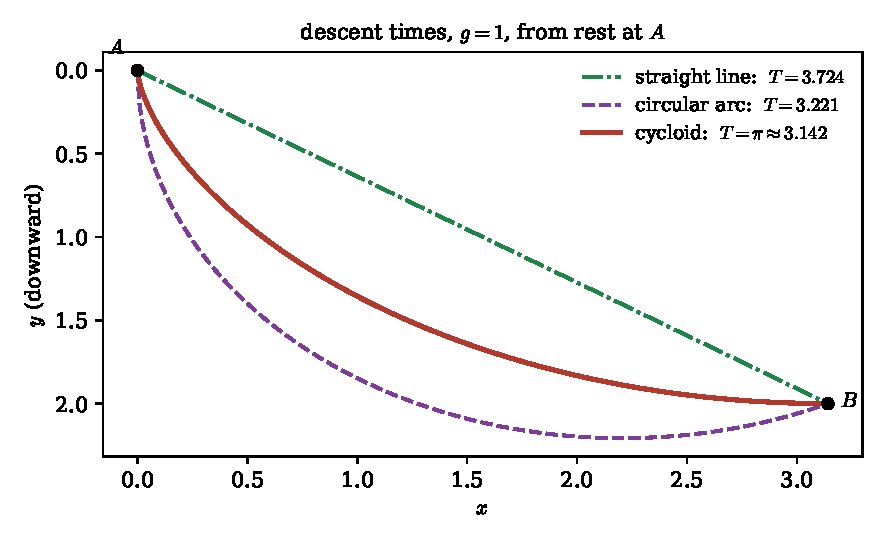
\includegraphics[width=0.85\textwidth]{fig_brachistochrone.pdf}
  \caption{Three wires from $A$ to $B = (\pi, 2)$ and their descent times
  (computed numerically from \eqref{eq:brachisto-functional} with $g=1$;
  the cycloid's time is exactly $\pi\sqrt{a/g}$). The straight line is
  shortest and slowest; the cycloid trades extra length for early speed
  and wins.}
  \label{fig:brachistochrone}
\end{figure}

\begin{remark}[Two bonuses of the parametrization]
(i) Along the cycloid the travel-time element collapses beautifully: with
$\dd s = 2a\sin(\theta/2)\,\dd\theta$ and
$v = \sqrt{2gy} = 2\sqrt{ga}\,\sin(\theta/2)$,
\begin{equation}
  \dd T = \frac{\dd s}{v} = \sqrt{\frac{a}{g}}\;\dd\theta
  \quad\Longrightarrow\quad
  T = \sqrt{\frac{a}{g}}\;\theta_B :
\end{equation}
the bead consumes \emph{equal times for equal parameter intervals}.
(ii) Releasing the bead from rest anywhere on the same cycloid, the time
to reach the bottom is the same --- the cycloid is also the
\emph{tautochrone}, the fact Huygens built into pendulum clocks. We state
(ii) without proof; it is a short exercise from (i)'s machinery.
\end{remark}

\begin{remark}[Bernoulli's own solution: physics borrowed from optics]
Johann Bernoulli solved the problem in 1697 without the Euler--Lagrange
equation (which did not yet exist) by a physical translation: the bead's
speed $v = \sqrt{2gy}$ depends only on depth, exactly like light in a
stratified medium with index $n(y) \propto 1/v \propto 1/\sqrt{y}$. By
Fermat's principle (\S\ref{sec:two-problems}), the least-time path of the
bead must be the path such light would take --- and Snell's law,
$\sin\alpha / v = \text{const}$ layer by layer, is then a ready-made first
integral. Writing $\sin\alpha = 1/\sqrt{1+y'^2}$ for a graph reproduces
precisely our Beltrami result $y(1+y'^2) = \text{const}$. The calculus
of variations is the common language in which
the optical and mechanical statements are the same statement.
\end{remark}

\subsection{Constrained problems and the catenary}
\label{sec:catenary-solution}

One opening problem remains, and it is the one the plain machinery
cannot yet touch: the catenary \eqref{eq:catenary-functional} adds a new
structural feature ---
the constraint is itself a functional (an \emph{isoperimetric}
constraint) --- and closing it will add the last general-purpose tool of
the section.
The resolution is the infinite-dimensional version of Lagrange multipliers.

\begin{theorem}[Isoperimetric multiplier rule]\label{thm:isoperimetric}
Let $J[y] = \int_a^b F\,\dd x$ and $\Lambda[y] = \int_a^b G\,\dd x$ with
$F, G$ of class $C^2$, and suppose $y_\ast$ is stationary for $J$ among
curves in $\mathcal C$ satisfying $\Lambda[y] = L$. If $y_\ast$ is
\emph{not} an unconstrained extremal of $\Lambda$ itself, then there
exists a constant $\lambda \in \R$ such that $y_\ast$ satisfies the
Euler--Lagrange equation of the \emph{combined} integrand
\begin{equation}
  \widetilde F \;=\; F + \lambda\, G .
\end{equation}
\end{theorem}

The logic (full proof: Appendix~\ref{app:isoperimetric}): with a
constraint, one cannot vary in every direction $\eta$ --- only in
directions that keep $\Lambda$ fixed to first order. A two-parameter
variation $y + \varepsilon_1\eta_1 + \varepsilon_2\eta_2$, with $\eta_2$
chosen to ``repair'' the constraint violation caused by $\eta_1$, shows
that $\delta J$ must be proportional to $\delta\Lambda$ direction by
direction; the proportionality constant is $\lambda$. This is exactly the
finite-dimensional picture --- $\nabla f \parallel \nabla g$ on a
constraint surface --- promoted to function space. The hypothesis that
$y_\ast$ not extremize $\Lambda$ is the nondegeneracy condition
($\nabla g \neq 0$) in disguise.

\paragraph{Solving the catenary.}
With $F = \mu g\, y\sqrt{1+y'^2}$ and $G = \sqrt{1+y'^2}$, absorb
constants and set
\begin{equation}
  \widetilde F = (y + \lambda)\,\sqrt{1 + y'^2},
\end{equation}
(the multiplier shifts the height --- already a hint of its physical
meaning). No explicit $x$: Beltrami applies.
\begin{equation}
  \pd{\widetilde F}{y'} = \frac{(y+\lambda)\,y'}{\sqrt{1+y'^2}},
  \qquad
  \widetilde F - y'\pd{\widetilde F}{y'}
  = (y+\lambda)\!\left[\sqrt{1+y'^2} - \frac{y'^2}{\sqrt{1+y'^2}}\right]
  = \frac{y+\lambda}{\sqrt{1+y'^2}} = C .
\end{equation}
Hence $(y+\lambda)^2 = C^2(1 + y'^2)$, i.e.
\begin{equation}
  y' = \sqrt{\frac{(y+\lambda)^2}{C^2} - 1}\,.
\end{equation}
Substitute $y + \lambda = C\cosh u$: then $\dd y = C\sinh u\,\dd u$ and
$y' = \sqrt{\cosh^2 u - 1} = \sinh u$, so
\begin{equation}
  C \sinh u\,\frac{\dd u}{\dd x} = \sinh u
  \quad\Longrightarrow\quad
  \frac{\dd u}{\dd x} = \frac1C
  \quad\Longrightarrow\quad
  u = \frac{x - x_0}{C},
\end{equation}
\begin{equation}
  \boxed{\;
  y(x) = C \cosh\!\left(\frac{x - x_0}{C}\right) - \lambda
  \;}
\end{equation}
--- the \emph{catenary}. The three constants $(C, x_0, \lambda)$ are fixed
by the two endpoint conditions and the length constraint $\Lambda[y]=L$.
Not a parabola: $\cosh$ and a parabola agree to quadratic order at the
bottom and then part ways (Fig.~\ref{fig:catenary}), which is why
Galileo's guess survived casual inspection for half a century.

\begin{figure}[ht]
  \centering
  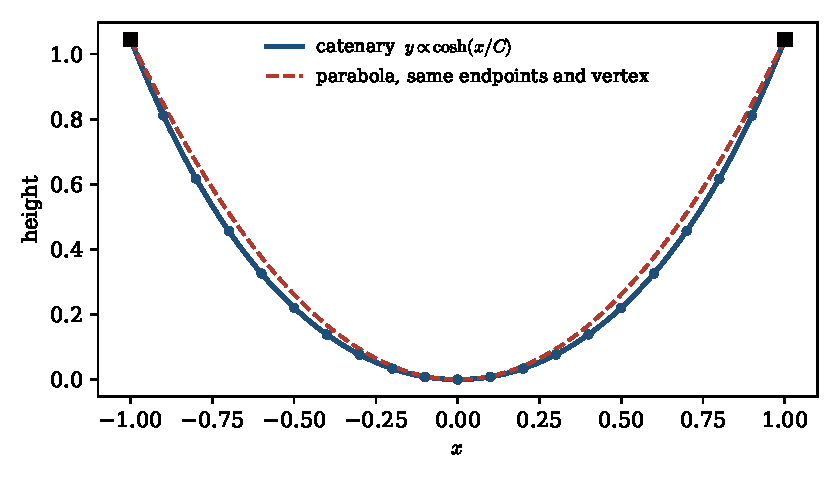
\includegraphics[width=0.8\textwidth]{fig_catenary.pdf}
  \caption{The catenary against the parabola with the same endpoints and
  vertex: close near the bottom (they share the quadratic term), visibly
  different toward the supports.}
  \label{fig:catenary}
\end{figure}

\begin{remark}[The physical meaning of the multiplier]
$\lambda$ entered as bookkeeping and exits with a job: comparing with the
statics of a hanging chain, $C = H/(\mu g)$ where $H$ is the horizontal
component of the chain's tension (constant along the chain), and $\lambda$
fixes the reference height at which the potential-plus-constraint
total balances. Multipliers of constraints are \emph{forces of
constraint} in embryo --- a theme \S\ref{sec:constraints} makes precise.
\end{remark}

\subsection{Covariance: why arbitrary coordinates are allowed}
\label{sec:covariance}

One more structural theorem before mechanics --- the one that makes
everything that follows practical.

\begin{theorem}[Covariance of the Euler--Lagrange equations]
\label{thm:covariance}
Let $Q_i = Q_i(q_1,\dots,q_n,\,t)$, $i = 1,\dots,n$, be a $C^2$ change of
coordinates with $C^2$ inverse, and let $\widetilde L$ be $L$ rewritten in
the new coordinates:
$\widetilde L(Q, \dot Q, t) = L\bigl(q(Q,t), \dot q(Q,\dot Q,t), t\bigr)$.
Then a curve satisfies the Euler--Lagrange equations for $L$ in the $q$'s
\emph{if and only if} its image satisfies the Euler--Lagrange equations for
$\widetilde L$ in the $Q$'s.
\end{theorem}

Proof in Appendix~\ref{app:covariance} (two chain-rule identities and a
cancellation). The content is one sentence:
\emph{the Euler--Lagrange equations do not care which coordinates you use}.
Newton's equations, by contrast, hold in Cartesian coordinates and mutate
under coordinate change (centrifugal and Coriolis terms in polar
coordinates, etc.). The variational formulation is coordinate-blind
because the underlying object --- ``this curve makes $\int L\,\dd t$
stationary'' --- never mentions coordinates at all: stationarity is a
property of the \emph{curve}, and \eqref{eq:EL} is merely its expression
in whichever chart is convenient. This theorem is the license behind the
phrase \emph{generalized coordinates}: angles, distances, differences of
angles --- anything that smoothly labels configurations is as good as $x$,
$y$, $z$.

%=======================================================================
\section{From Newton to Lagrange}
%=======================================================================
\label{sec:newton-lagrange}

Why rebuild mechanics, when $\vec F = m\vec a$ already works? Because
Newton's formulation, for all its power, has three practical irritations
and hides one deep structure. The irritations: it is wedded to
\emph{vectors in Cartesian coordinates} (change to polar coordinates and
fictitious terms sprout); it forces you to carry \emph{constraint forces}
--- rod tensions, normal forces --- as unknowns you must solve for and
rarely want; and its symmetries are \emph{invisible} --- nothing in the
notation $m\ddot{\vr} = \vec F$ announces that momentum conservation is
the same fact as the homogeneity of space. The variational reformulation
answers all three at once: Theorem~\ref{thm:covariance} makes any
coordinates legal, the treatment of constraints below makes constraint
forces vanish before the calculation starts, and Noether's theorem
(\S\ref{sec:conservation}) turns symmetry into conservation by a two-line
argument. The deep structure it exposes --- one scalar function $L$
generating all equations of motion, the dynamics as a stationarity
condition on whole histories --- is the form in which mechanics
generalizes: field theory, relativity, and quantum mechanics are all
written in this language, not in Newton's. The cost is one
new postulate, which we now state and immediately check against Newton.

\subsection{Hamilton's principle}
\label{sec:hamilton-principle}

\begin{definition}[Lagrangian and action]
For a mechanical system described by coordinates
$\vq = (q_1,\dots,q_n)$, the \emph{Lagrangian} is
\begin{equation}
  \boxed{\;L(\vq, \dot\vq, t) = T - V\;}
\end{equation}
kinetic minus potential energy, and the \emph{action} of a trajectory
$\vq(t)$ on $[t_0, t_1]$ is the functional
\begin{equation}
  \boxed{\;
  S[\vq] = \int_{t_0}^{t_1} L\bigl(\vq(t), \dot\vq(t), t\bigr)\,\dd t .
  \;}
\end{equation}
\end{definition}

\begin{postulate}[Hamilton's principle of stationary action]
\label{post:hamilton}
The physical trajectory between fixed configurations
$\vq(t_0) = \vq_A$ and $\vq(t_1) = \vq_B$ is a stationary point of the
action: $\delta S = 0$.
\end{postulate}

By Theorem~\ref{thm:EL} in its several-function form
(Remark~\ref{rem:vector-EL}, with $x \to t$), the postulate is equivalent
to the \emph{Euler--Lagrange equations of motion}
\begin{equation}
  \boxed{\;
  \frac{\dd}{\dd t}\pd{L}{\dot q_i} - \pd{L}{q_i} = 0,
  \qquad i = 1, \dots, n .
  \;}
  \label{eq:EL-mech}
\end{equation}

\paragraph{First duty: recover Newton.}
A postulate must first reproduce what is known. Take one particle
in Cartesian coordinates, $V = V(\vr)$:
\begin{equation}
  L = \tfrac12 m\bigl(\dot x^2 + \dot y^2 + \dot z^2\bigr) - V(x,y,z).
\end{equation}
For the $x$-equation:
\begin{equation}
  \pd{L}{\dot x} = m\dot x,
  \qquad
  \frac{\dd}{\dd t}\pd{L}{\dot x} = m\ddot x,
  \qquad
  \pd{L}{x} = -\pd{V}{x} = F_x ,
\end{equation}
so \eqref{eq:EL-mech} reads $m\ddot x = F_x$, and likewise for $y, z$:
\begin{equation}
  m\ddot\vr = -\nabla V = \vec F .
\end{equation}
Newton's second law, exactly. \emph{For unconstrained conservative systems
in Cartesian coordinates, Hamilton's principle and Newton's law are the
same statement.} Everything the new formulation adds --- and it adds a
great deal --- comes from the two theorems already in hand:
covariance (Theorem~\ref{thm:covariance}: use any coordinates) and the
treatment of constraints (next).

\begin{remark}[Why $T - V$? The accounting, plus an intuition]
The \emph{minus} sign is not derivable from anything prior in this
document: $L = T - V$ is part of the postulate, and its justification is
exactly the check just performed --- it is the choice that reproduces
Newton. (Try $T + V$: the sign of the force flips.) That said, the
combination can be \emph{felt}. Take a thrown ball, and grant for
intuition's sake that its short arcs \emph{minimize} the action
$\int (T - V)\,\dd t$ (true for sufficiently short arcs;
Convention~\ref{conv:stationary} guards the general statement). The
integrand is lowered by spending time where $V$ is \emph{high} --- so the
path bulges upward, lingering near the top of its flight --- but height
requires speed on the way up and down, and speed raises the kinetic
term. Bulge
too little and the $-V$ reduction is wasted; bulge too much and the
kinetic cost dominates. The parabola is the balance point of this
trade-off, and
the Euler--Lagrange equation is the statement that the balance holds at
every instant separately. This is intuition, not derivation --- the
derivation is the check above --- but it is the right picture to carry.
\end{remark}

\subsection{Constraints and generalized coordinates}
\label{sec:constraints}

Real systems are full of constraints: the pendulum bob stays on its rod,
the bead stays on its wire, the chain link stays attached to its neighbor.
The Newtonian treatment must carry the \emph{constraint forces} (rod
tension, wire normal force) as unknowns and solve for them. The Lagrangian
treatment makes them vanish from the outset. Here is the physics of why,
kept in full in the main text because it \emph{is} the key step.

\paragraph{Setup.}
Let a system of $N$ particles $\vr_a$ ($a = 1,\dots,N$) be subject to
\emph{holonomic} constraints --- conditions on positions (possibly time),
$f_\alpha(\vr_1,\dots,\vr_N, t) = 0$ --- which are enforced by constraint
forces $\vec C_a$, so that Newton reads
\begin{equation}
  m_a \ddot\vr_a = \vec F_a + \vec C_a
  \qquad (\vec F_a = -\nabla_a V \text{ the applied forces}).
  \label{eq:newton-constrained}
\end{equation}
Suppose the constraint surface is smoothly parametrized by $n$
\emph{generalized coordinates}:
$\vr_a = \vr_a(q_1,\dots,q_n, t)$.

\begin{postulate}[Ideal constraints / d'Alembert]\label{post:dalembert}
The constraint forces do no work under any \emph{virtual displacement} ---
any infinitesimal displacement consistent with the constraints at frozen
time:
\begin{equation}
  \sum_{a=1}^N \vec C_a \cdot \pd{\vr_a}{q_i} = 0
  \qquad \text{for each } i .
\end{equation}
\end{postulate}

This is a physical assumption, and an excellent one: rods, frictionless
wires, and rigid links push only \emph{perpendicular} to the motions they
permit --- that is what ``rigid and frictionless'' means. (Sliding
friction violates it; such forces must be kept explicitly.)

\paragraph{The computation.}
Take Newton \eqref{eq:newton-constrained}, dot each equation with
$\partial\vr_a/\partial q_i$, and sum over particles. The constraint
forces drop by Postulate~\ref{post:dalembert}:
\begin{equation}
  \sum_a m_a \ddot\vr_a\cdot\pd{\vr_a}{q_i}
  = \sum_a \vec F_a \cdot \pd{\vr_a}{q_i}
  \;\equiv\; \mathcal{Q}_i
  \qquad(\text{the \emph{generalized force}}).
  \label{eq:projected-newton}
\end{equation}
The left side is reorganized by two kinetic identities. From the chain
rule, $\dot\vr_a = \sum_j \pd{\vr_a}{q_j}\dot q_j + \pd{\vr_a}{t}$, whence
\begin{equation}
  \text{(K1)}\quad \pd{\dot\vr_a}{\dot q_i} = \pd{\vr_a}{q_i},
  \qquad\qquad
  \text{(K2)}\quad \frac{\dd}{\dd t}\pd{\vr_a}{q_i} = \pd{\dot\vr_a}{q_i}
\end{equation}
--- (K1) because $\dot q_i$ enters $\dot\vr_a$ linearly with coefficient
$\partial\vr_a/\partial q_i$; (K2) because both sides equal
$\sum_j \tfrac{\partial^2\vr_a}{\partial q_j\partial q_i}\dot q_j
+ \tfrac{\partial^2 \vr_a}{\partial t\,\partial q_i}$ (mixed partials
commute for $C^2$ maps). Now write, by the product rule,
\begin{equation}
  \ddot\vr_a \cdot \pd{\vr_a}{q_i}
  = \frac{\dd}{\dd t}\!\left(\dot\vr_a\cdot\pd{\vr_a}{q_i}\right)
  - \dot\vr_a\cdot\frac{\dd}{\dd t}\pd{\vr_a}{q_i}
  \overset{\text{(K1),(K2)}}{=}
  \frac{\dd}{\dd t}\!\left(\dot\vr_a\cdot\pd{\dot\vr_a}{\dot q_i}\right)
  - \dot\vr_a\cdot\pd{\dot\vr_a}{q_i} .
\end{equation}
Multiply by $m_a$, sum over $a$, and recognize the kinetic energy
$T = \sum_a \tfrac12 m_a \dot\vr_a^{\,2}$ on both terms:
\begin{equation}
  \sum_a m_a\ddot\vr_a\cdot\pd{\vr_a}{q_i}
  = \frac{\dd}{\dd t}\pd{T}{\dot q_i} - \pd{T}{q_i}.
\end{equation}
If moreover the applied forces are conservative, $\vec F_a = -\nabla_a V$
with $V = V(\vr_1,\dots,\vr_N,t)$, then by the chain rule
$\mathcal{Q}_i = -\partial V/\partial q_i$, and since $V$ has no
$\dot q$-dependence, \eqref{eq:projected-newton} assembles into
\begin{equation}
  \frac{\dd}{\dd t}\pd{(T-V)}{\dot q_i} - \pd{(T-V)}{q_i} = 0 .
\end{equation}

\begin{theorem}[Lagrange's equations for constrained systems]
\label{thm:constrained-L}
For a system with ideal holonomic constraints and conservative applied
forces, the generalized coordinates obey the Euler--Lagrange equations
\eqref{eq:EL-mech} of $L = T - V$, \emph{with the constraint forces
nowhere appearing and the constraints automatically respected}.
\end{theorem}

The working recipe of Lagrangian mechanics, now fully justified:
\begin{center}
\fbox{\parbox{0.86\textwidth}{
\textbf{Recipe.} (1)~Choose any $n$ independent coordinates that label the
allowed configurations. (2)~Write $T$ and $V$ in them. (3)~Form $L = T-V$
and turn the Euler--Lagrange crank. Constraint forces never enter; if you
want them afterward (engineering loads!), reinstate the constrained
coordinate with a multiplier --- the multiplier \emph{is} the force, the
catenary's $\lambda$ writ general.}}
\end{center}

\subsection{Conservation laws}
\label{sec:conservation}

The variational structure converts symmetries into conserved quantities
with almost no work. Three instances, in increasing generality.

\paragraph{Cyclic coordinates.}
Define the \emph{generalized (canonical) momentum} conjugate to $q_i$:
\begin{equation}
  \boxed{\;p_i \equiv \pd{L}{\dot q_i}\;}
\end{equation}
If $L$ does not contain $q_i$ ($q_i$ is \emph{cyclic}), then
\eqref{eq:EL-mech} gives $\dot p_i = \partial L/\partial q_i = 0$:
\begin{equation}
  \boxed{\;q_i \text{ cyclic} \;\Longrightarrow\; p_i \text{ conserved.}\;}
\end{equation}
(Proposition~\ref{prop:cyclic} in mechanical clothing. Example: a free
particle, $L = \tfrac12 m\dot x^2$, has $x$ cyclic and $p = m\dot x$
conserved.)

\paragraph{Energy.}
Define the \emph{energy function}
\begin{equation}
  \boxed{\;
  h(\vq, \dot\vq, t) \;\equiv\; \sum_i \dot q_i\,\pd{L}{\dot q_i} \;-\; L .
  \;}
\end{equation}
\begin{proposition}\label{prop:energy}
Along any solution of \eqref{eq:EL-mech},
$\dfrac{\dd h}{\dd t} = -\dfrac{\partial L}{\partial t}$.
In particular, if $L$ has no explicit time dependence, $h$ is conserved.
\end{proposition}
\begin{proof}
Differentiate along the trajectory:
\begin{align}
  \frac{\dd h}{\dd t}
  &= \sum_i \ddot q_i \pd{L}{\dot q_i}
   + \sum_i \dot q_i \frac{\dd}{\dd t}\pd{L}{\dot q_i}
   - \left[\sum_i \pd{L}{q_i}\dot q_i
   + \sum_i \pd{L}{\dot q_i}\ddot q_i + \pd{L}{t}\right] \nonumber\\
  &= \sum_i \dot q_i\left[\frac{\dd}{\dd t}\pd{L}{\dot q_i}
     - \pd{L}{q_i}\right] - \pd{L}{t}
   = -\,\pd{L}{t},
\end{align}
the bracket vanishing by the equations of motion. (This is the Beltrami
identity, Proposition~\ref{prop:beltrami}, in $n$ variables: ``no explicit
$t$'' plays the role of ``no explicit $x$.'') Whether $h$ equals $T + V$
is a separate question answered precisely in \S\ref{sec:when-H-is-E};
and whether $h$ ``is'' the Hamiltonian is a sharper question than it
looks, answered precisely in Remark~\ref{rem:h-vs-H}.
\end{proof}

\paragraph{Noether's theorem.}
The two facts above are shadows of one statement: \emph{continuous
symmetries of $L$ produce conserved quantities}.

\begin{theorem}[Noether, point-symmetry version]\label{thm:noether}
Let $\vq \mapsto \vec Q(\vq, s)$ be a smooth one-parameter family of
transformations with $\vec Q(\vq, 0) = \vq$, and suppose it leaves the
Lagrangian invariant:
\begin{equation}
  L\bigl(\vec Q(\vq,s),\, \tfrac{\dd}{\dd t}\vec Q(\vq,s),\, t\bigr)
  = L(\vq, \dot\vq, t)
  \qquad\text{for all } s .
\end{equation}
Then, writing $\eta_i(\vq) = \dfrac{\partial Q_i}{\partial s}\Big|_{s=0}$
for the infinitesimal generator, the quantity
\begin{equation}
  \boxed{\;
  I \;=\; \sum_i \pd{L}{\dot q_i}\;\eta_i(\vq)
  \;}
\end{equation}
is conserved along every solution of the equations of motion.
\end{theorem}

\begin{proof}
Differentiate the invariance identity with respect to $s$ at $s=0$. Since
along the transformed family
$\tfrac{\partial}{\partial s}\dot Q_i\big|_{s=0} = \dot\eta_i$
(the $s$- and $t$-derivatives commute for smooth families),
\begin{equation}
  0 = \left.\frac{\dd}{\dd s}\right|_{0} L
  = \sum_i \pd{L}{q_i}\,\eta_i + \sum_i \pd{L}{\dot q_i}\,\dot\eta_i .
\end{equation}
So far this holds for any curve. Now evaluate \emph{on a solution} and use
the equations of motion to replace
$\partial L/\partial q_i = \tfrac{\dd}{\dd t}(\partial L/\partial\dot q_i)$:
\begin{equation}
  0 = \sum_i \left[\frac{\dd}{\dd t}\pd{L}{\dot q_i}\right]\eta_i
    + \sum_i \pd{L}{\dot q_i}\,\dot\eta_i
  = \frac{\dd}{\dd t}\left[\sum_i \pd{L}{\dot q_i}\,\eta_i\right]
  = \frac{\dd I}{\dd t}. \qedhere
\end{equation}
\end{proof}

\begin{example}[The classic pairs]
(i) \emph{Translation}: $Q = q + s$ for a coordinate absent from $L$;
$\eta = 1$, $I = p$. Cyclic coordinates are Noether's theorem for
translations in configuration space. (ii) \emph{Rotation}: a particle in a
central potential, $L = \tfrac12 m(\dot x^2 + \dot y^2) - V(\sqrt{x^2+y^2})$,
is invariant under $(x, y) \mapsto (x\cos s - y\sin s,\, x\sin s +
y\cos s)$; the generator is $\eta = (-y, x)$ and
\begin{equation}
  I = m\dot x\,(-y) + m\dot y\,(x) = m(x\dot y - y\dot x) = L_z ,
\end{equation}
angular momentum. (iii) Time translation stands slightly apart --- it
shifts the curve's parameter rather than its values, so it does not fit
the hypothesis of Theorem~\ref{thm:noether} as stated --- and its
conserved quantity is exactly the $h$ of
Proposition~\ref{prop:energy}, whose proof is the time-translation
analogue of the argument above. The moral is
uniform: \textbf{momentum is the charge of spatial translation, angular
momentum of rotation, energy of time translation.}
\end{example}

\begin{example}[Central forces: the effective one-dimensional
problem]\label{ex:central-force}
The cyclic-coordinate machinery at full power. A particle in a plane
under $V = V(r)$ (planar without loss for a central force: angular
momentum fixes the orbital plane [stated; it follows from conservation
of the vector angular momentum $m\,\vr\times\dot\vr$]), in polar
coordinates:
\begin{equation}
  L = \tfrac12 m\bigl(\dot r^2 + r^2\dot\varphi^2\bigr) - V(r).
\end{equation}
The angle is cyclic, so its momentum is conserved,
\begin{equation}
  p_\varphi = \pd{L}{\dot\varphi} = m r^2\dot\varphi \equiv \ell
  = \text{const},
\end{equation}
and the conserved energy $h = T + V$ (constraints time-independent),
with $\dot\varphi$ eliminated via $\dot\varphi = \ell/mr^2$, becomes
\begin{equation}
  \boxed{\;
  E = \tfrac12 m\dot r^2
  + \underbrace{\frac{\ell^2}{2m r^2} + V(r)}_{\displaystyle
    V_{\text{eff}}(r)}
  \;}
\end{equation}
--- a \emph{one-dimensional} problem on the half-line $r > 0$, with
the conserved angular momentum converted into a repulsive
\emph{centrifugal barrier} $\ell^2/2mr^2$. Circular orbits sit at
$V_{\text{eff}}'(r_0) = 0$, stable where $V_{\text{eff}}'' > 0$; the
full radial motion is read off the one-dimensional energy diagram
exactly as in \S\ref{sec:phase-space}. One warning, displayed
because it is the step a reader gets wrong: eliminate $\dot\varphi$
in the \emph{energy}, not in the Lagrangian --- substituting
$\dot\varphi = \ell/mr^2$ into $L$ before varying flips the sign of
the centrifugal term in the resulting equation of motion [the
correct reduction at the Lagrangian level is the Routhian; stated].
(The quantum version of this reduction, with $\ell^2$ replaced by
$\ell(\ell+1)\hbar^2$, is the radial equation of the quantum
companion.)
\end{example}

%=======================================================================
\section{The Pendulum}
%=======================================================================
\label{sec:pendulum}

The recipe of \S\ref{sec:constraints}, run start to finish on the simplest
constrained system --- one rigid rod, one angle. The point of the exercise
is partly the result (the harmonic oscillator's most venerable
realization) but mostly the \emph{silence}: watch for what never appears
in the calculation.

\subsection{Setup and equation of motion}

A bob of mass $m$ on a rigid massless rod of length $\ell$, pivoting
freely in a vertical plane; uniform gravity $g$.

\begin{center}
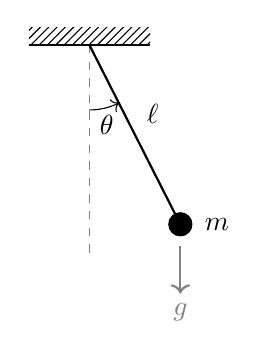
\begin{tikzpicture}[scale=1.1]
  \fill[pattern=north east lines] (-0.7,0.12) rectangle (0.7,0.32);
  \draw[thick] (-0.7,0.12) -- (0.7,0.12);
  \draw[gray, dashed] (0,0.12) -- (0,-2.3);
  \draw[thick] (0,0.12) -- (1.05,-1.95);
  \fill (1.05,-1.95) circle (0.14);
  \node[right] at (1.22,-1.95) {$m$};
  \node[right] at (0.55,-0.68) {$\ell$};
  \draw[->] (0,-0.63) arc (270:297:0.75);
  \node at (0.20,-0.80) {$\theta$};
  \draw[->, thick, gray] (1.05,-2.2) -- (1.05,-2.75) node[below] {$g$};
\end{tikzpicture}
\end{center}

The constraint (fixed distance $\ell$ from the pivot) is holonomic and
ideal (the rod's force lies along itself, perpendicular to the circular
motion). One generalized coordinate suffices: the angle $\theta$ from the
downward vertical. Cartesian positions and velocities:
\begin{equation}
  x = \ell\sin\theta,\quad y = -\ell\cos\theta
  \qquad\Longrightarrow\qquad
  \dot x = \ell\cos\theta\,\dot\theta,\quad
  \dot y = \ell\sin\theta\,\dot\theta,
\end{equation}
\begin{equation}
  T = \tfrac12 m(\dot x^2 + \dot y^2)
    = \tfrac12 m\ell^2\dot\theta^2
    \bigl(\cos^2\theta + \sin^2\theta\bigr)
    = \tfrac12 m \ell^2 \dot\theta^2,
  \qquad
  V = mgy = -\,mg\ell\cos\theta .
\end{equation}
\begin{equation}
  \boxed{\;
  L(\theta, \dot\theta)
  = \tfrac12 m\ell^2\dot\theta^2 + mg\ell\cos\theta
  \;}
\end{equation}
Euler--Lagrange:
\begin{equation}
  \pd{L}{\dot\theta} = m\ell^2\dot\theta,
  \qquad
  \frac{\dd}{\dd t}\pd{L}{\dot\theta} = m\ell^2\ddot\theta,
  \qquad
  \pd{L}{\theta} = -mg\ell\sin\theta ,
\end{equation}
\begin{equation}
  \boxed{\;
  \ddot\theta = -\,\frac{g}{\ell}\,\sin\theta
  \;}
  \label{eq:pendulum-eom}
\end{equation}
Note what did \emph{not} happen: the rod tension was never introduced,
never computed, never eliminated --- the coordinate $\theta$ respects the
constraint by construction, and Theorem~\ref{thm:constrained-L} did the
rest. (Compare the Newtonian route: decompose gravity along and across the
rod, introduce the tension, project. Same result, more work, and
the work multiplies with each additional constraint --- as
\S\ref{sec:double-pendulum} is about to demonstrate by its absence.)

\subsection{Small angles: the harmonic oscillator recovered}

For $|\theta| \ll 1$, $\sin\theta = \theta + O(\theta^3)$, and
\eqref{eq:pendulum-eom} linearizes to
\begin{equation}
  \ddot\theta = -\,\omega_0^2\,\theta,
  \qquad
  \omega_0 = \sqrt{\frac{g}{\ell}}
\end{equation}
--- the simple harmonic oscillator, whose complete theory (solution
forms, energy, damping, driving, resonance) is the subject of the
companion oscillator reference and is reused here wholesale. Period
$T = 2\pi\sqrt{\ell/g}$, independent of amplitude and of mass.

\begin{remark}[Beyond small angles]\label{rem:exact-pendulum}
Equation \eqref{eq:pendulum-eom} is exactly solvable, but not in
elementary functions: conservation of $h$ gives
$\tfrac12\ell\dot\theta^2 = g(\cos\theta - \cos\theta_{\max})$, and
separating variables produces a period
\begin{equation}
  T(\theta_{\max})
  = 4\sqrt{\frac{\ell}{g}}\,K\!\Bigl(\sin\tfrac{\theta_{\max}}{2}\Bigr),
  \qquad
  K(k) = \int_0^{\pi/2}\frac{\dd\varphi}{\sqrt{1 - k^2\sin^2\varphi}} ,
\end{equation}
a complete elliptic integral. Expanding:
$T = 2\pi\sqrt{\ell/g}\,\bigl(1 + \tfrac{1}{16}\theta_{\max}^2 +
O(\theta_{\max}^4)\bigr)$ --- the period grows with amplitude, by about
$1.7\%$ at $\theta_{\max} = 30^\circ$. The isochronism of
\S\ref{sec:pendulum} is the $\theta^2$-truncation speaking, not the
pendulum. (The curve that \emph{is} exactly isochronous is the cycloid of
\S\ref{sec:brachisto-solution} --- the tautochrone; the subject's opening
problem and its first mechanical example are secretly the same curve.)
\end{remark}

%=======================================================================
\section{The Double Pendulum at Small Angles}
%=======================================================================
\label{sec:double-pendulum}

The first system where the Lagrangian route is decisively easier.
Attempt this system
in Newtonian style and you will meet two unknown rod tensions, one of
which acts on a bob that is itself accelerating in a curved path
determined by the other --- a genuinely unpleasant exercise in algebra.
The Lagrangian route needs eleven lines of kinematics and two derivatives.
The system is also the smallest one exhibiting two structural novelties:
a kinetic energy that is \emph{not} a sum of squares (the mass matrix
acquires off-diagonal terms), which will force the correct
generalization
of the eigenvalue problem; and, beyond small angles, deterministic chaos
(\S\ref{sec:outlook}) --- all from two rods and two bobs.

\subsection{Setup and kinematics}

Bob 1 (mass $m_1$) hangs from the pivot on a rod of length $\ell_1$;
bob 2 (mass $m_2$) hangs from bob 1 on a rod of length $\ell_2$. Angles
$\theta_1, \theta_2$ from the vertical.

\begin{center}
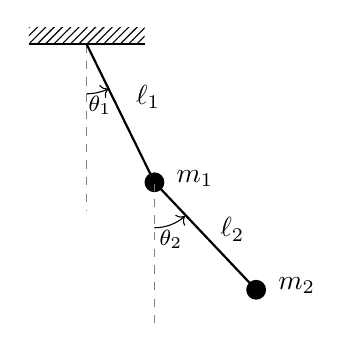
\begin{tikzpicture}[scale=1.05]
  \fill[pattern=north east lines] (-0.7,0.12) rectangle (0.7,0.32);
  \draw[thick] (-0.7,0.12) -- (0.7,0.12);
  \draw[gray, dashed] (0,0.12) -- (0,-1.9);
  \draw[thick] (0,0.12) -- (0.82,-1.55);
  \fill (0.82,-1.55) circle (0.12);
  \node[right] at (0.97,-1.5) {$m_1$};
  \node[right] at (0.48,-0.52) {$\ell_1$};
  \draw[->] (0,-0.48) arc (270:296:0.6);
  \node at (0.16,-0.62) {\footnotesize $\theta_1$};
  \draw[gray, dashed] (0.82,-1.55) -- (0.82,-3.3);
  \draw[thick] (0.82,-1.55) -- (2.05,-2.85);
  \fill (2.05,-2.85) circle (0.12);
  \node[right] at (2.2,-2.8) {$m_2$};
  \node[right] at (1.50,-2.12) {$\ell_2$};
  \draw[->] (0.82,-2.10) arc (270:312:0.55);
  \node at (1.02,-2.24) {\footnotesize $\theta_2$};
\end{tikzpicture}
\end{center}

Positions ($y$ upward from the pivot):
\begin{align}
  x_1 &= \ell_1\sin\theta_1, & y_1 &= -\ell_1\cos\theta_1, \\
  x_2 &= \ell_1\sin\theta_1 + \ell_2\sin\theta_2, &
  y_2 &= -\ell_1\cos\theta_1 - \ell_2\cos\theta_2 .
\end{align}
Velocities by the chain rule:
\begin{align}
  \dot x_2 &= \ell_1\cos\theta_1\,\dot\theta_1 + \ell_2\cos\theta_2\,\dot\theta_2,
  \qquad
  \dot y_2 = \ell_1\sin\theta_1\,\dot\theta_1 + \ell_2\sin\theta_2\,\dot\theta_2 ,
\end{align}
and the speed of bob 2, expanded carefully (the cross term is the whole
story of this system):
\begin{align}
  \dot x_2^2 + \dot y_2^2
  &= \ell_1^2\dot\theta_1^2\,(\cos^2\theta_1 + \sin^2\theta_1)
   + \ell_2^2\dot\theta_2^2\,(\cos^2\theta_2 + \sin^2\theta_2) \nonumber\\
  &\quad + 2\ell_1\ell_2\dot\theta_1\dot\theta_2\,
    (\cos\theta_1\cos\theta_2 + \sin\theta_1\sin\theta_2) \nonumber\\
  &= \ell_1^2\dot\theta_1^2 + \ell_2^2\dot\theta_2^2
   + 2\ell_1\ell_2\,\cos(\theta_1 - \theta_2)\,\dot\theta_1\dot\theta_2 .
\end{align}
Hence
\begin{align}
  T &= \tfrac12 m_1\ell_1^2\dot\theta_1^2
     + \tfrac12 m_2\Bigl[\ell_1^2\dot\theta_1^2 + \ell_2^2\dot\theta_2^2
     + 2\ell_1\ell_2\cos(\theta_1{-}\theta_2)\,\dot\theta_1\dot\theta_2\Bigr], \\
  V &= -\,(m_1{+}m_2)\,g\ell_1\cos\theta_1 \;-\; m_2 g\ell_2\cos\theta_2 ,
\end{align}
and $L = T - V$. Pause on what was \emph{not} needed: neither rod tension
appears, no forces were decomposed, no free-body diagram of bob 2 in the
accelerating frame of bob 1 was contemplated. The two constraints cost
nothing.

\subsection{Exact equations of motion}

Write $\Delta \equiv \theta_1 - \theta_2$. For $\theta_1$:
\begin{align}
  \pd{L}{\dot\theta_1}
  &= (m_1{+}m_2)\ell_1^2\dot\theta_1
   + m_2\ell_1\ell_2\cos\Delta\;\dot\theta_2, \\
  \frac{\dd}{\dd t}\pd{L}{\dot\theta_1}
  &= (m_1{+}m_2)\ell_1^2\ddot\theta_1
   + m_2\ell_1\ell_2\cos\Delta\;\ddot\theta_2
   - m_2\ell_1\ell_2\sin\Delta\;(\dot\theta_1 - \dot\theta_2)\,\dot\theta_2, \\
  \pd{L}{\theta_1}
  &= -\,m_2\ell_1\ell_2\sin\Delta\;\dot\theta_1\dot\theta_2
   \;-\; (m_1{+}m_2)\,g\ell_1\sin\theta_1 ,
\end{align}
and the Euler--Lagrange equation, after the two $\sin\Delta$ terms
combine,
\begin{equation}
  (m_1{+}m_2)\ell_1^2\,\ddot\theta_1
  + m_2\ell_1\ell_2\cos\Delta\;\ddot\theta_2
  + m_2\ell_1\ell_2\sin\Delta\;\dot\theta_2^{\,2}
  + (m_1{+}m_2)\,g\ell_1\sin\theta_1 = 0 .
  \label{eq:dp-exact-1}
\end{equation}
For $\theta_2$, the same procedure ($\partial L/\partial\theta_2$ picks up
$+m_2\ell_1\ell_2\sin\Delta\,\dot\theta_1\dot\theta_2$, note the sign)
gives
\begin{equation}
  m_2\ell_2^2\,\ddot\theta_2
  + m_2\ell_1\ell_2\cos\Delta\;\ddot\theta_1
  - m_2\ell_1\ell_2\sin\Delta\;\dot\theta_1^{\,2}
  + m_2\,g\ell_2\sin\theta_2 = 0 .
  \label{eq:dp-exact-2}
\end{equation}
These exact equations are nonlinear, coupled, and --- as
\S\ref{sec:outlook} notes --- chaotic at large amplitude. Our target is
their small-angle limit.

\subsection{Linearization done in the right order}
\label{sec:linearization}

Small oscillations about the hanging equilibrium: $\theta_i$,
$\dot\theta_i$ all first-order small. There are two natural procedures ---
(a) linearize the exact equations
\eqref{eq:dp-exact-1}--\eqref{eq:dp-exact-2}, or (b) truncate $L$ at
quadratic order and \emph{then} apply Euler--Lagrange --- and it deserves
one displayed sentence that they agree:

\begin{lemma}[Expand-then-vary equals vary-then-expand]
\label{lem:order-of-operations}
The Euler--Lagrange equations of the quadratic truncation $L_2$ of $L$
about an equilibrium coincide with the linearization of the
Euler--Lagrange equations of $L$ about that equilibrium.
\end{lemma}
\begin{proof}
Euler--Lagrange takes one derivative of $L$ in each slot; hence terms of
cubic and higher order in $(\vth, \dot\vth)$ in $L$ produce terms of
quadratic and higher order in the equations, which the linearization
discards. Conversely every quadratic term of $L$ survives one
differentiation as a linear term. The two truncations remove exactly the
same terms.
\end{proof}

Route (b) is less error-prone (truncate once, differentiate a polynomial).
Truncate: $\cos\Delta = 1 + O(\Delta^2)$ multiplies
$\dot\theta_1\dot\theta_2$, already second order, so the correction is
fourth order --- drop it; $\cos\theta_i = 1 - \tfrac12\theta_i^2 +
O(\theta_i^4)$ in $V$; discard constants. The quadratic Lagrangian:
\begin{equation}
  L_2 =
  \tfrac12(m_1{+}m_2)\ell_1^2\dot\theta_1^2
  + \tfrac12 m_2\ell_2^2\dot\theta_2^2
  + m_2\ell_1\ell_2\,\dot\theta_1\dot\theta_2
  - \tfrac12(m_1{+}m_2)g\ell_1\,\theta_1^2
  - \tfrac12 m_2 g\ell_2\,\theta_2^2 .
\end{equation}
Euler--Lagrange on this polynomial (each derivative now trivial):
\begin{align}
  (m_1{+}m_2)\ell_1^2\,\ddot\theta_1 + m_2\ell_1\ell_2\,\ddot\theta_2
  &= -\,(m_1{+}m_2)g\ell_1\,\theta_1, \nonumber\\
  m_2\ell_1\ell_2\,\ddot\theta_1 + m_2\ell_2^2\,\ddot\theta_2
  &= -\,m_2 g\ell_2\,\theta_2 ,
\end{align}
i.e., in matrix form,
\begin{equation}
  \boxed{\;
  \mM\,\ddot{\vth} = -\,\mK\,\vth,
  \qquad
  \mM =
  \begin{pmatrix}
    (m_1{+}m_2)\ell_1^2 & m_2\ell_1\ell_2\\
    m_2\ell_1\ell_2 & m_2\ell_2^2
  \end{pmatrix},
  \quad
  \mK =
  \begin{pmatrix}
    (m_1{+}m_2)g\ell_1 & 0\\
    0 & m_2 g\ell_2
  \end{pmatrix}
  \;}
  \label{eq:dp-matrix}
\end{equation}
Both matrices are symmetric --- $\mM$ from the quadratic form $T$, $\mK$
from the quadratic form $V$ --- and both are positive definite ($T > 0$
for any nonzero velocity; $V$ has a strict minimum at hanging
equilibrium). But unlike every system in the oscillator companion,
\emph{the mass matrix is not diagonal}: the kinetic cross term
$\dot\theta_1\dot\theta_2$ couples the coordinates through their
\emph{velocities}. The plain eigenvalue problem no longer applies; its
correct generalization is next.

\subsection{The generalized eigenvalue problem}
\label{sec:gevp}

Insert the oscillatory ansatz $\vth(t) = \vec v\,\cos(\omega t - \phi)$
into \eqref{eq:dp-matrix}:
\begin{equation}
  -\,\omega^2\,\mM\,\vec v\,\cos(\omega t - \phi)
  = -\,\mK\,\vec v\,\cos(\omega t - \phi)
  \quad\Longleftrightarrow\quad
  \boxed{\;\mK\,\vec v = \omega^2\,\mM\,\vec v\;}
  \label{eq:gevp}
\end{equation}
--- a \emph{generalized} eigenvalue problem: $\mM$ stands where the
identity used to. Nontrivial $\vec v$ requires
\begin{equation}
  \det\bigl(\mK - \omega^2 \mM\bigr) = 0 .
\end{equation}
The general theory is exactly as strong as in the ordinary case:

\begin{theorem}[Normal modes exist and diagonalize the system]
\label{thm:simultaneous}
Let $\mM$ be symmetric positive definite and $\mK$ symmetric ($n\times n$,
real). Then \eqref{eq:gevp} has $n$ real eigenvalues
$\omega_1^2 \le \dots \le \omega_n^2$ (positive if $\mK$ is positive
definite) with eigenvectors $\vec v_1,\dots,\vec v_n$ that form a basis
and are orthogonal in the $\mM$-inner product,
$\vec v_r^{\mathsf T}\mM\,\vec v_s = 0$ for $r\ne s$. In the coordinates
$\vth = \sum_r \xi_r \vec v_r$, the system \eqref{eq:dp-matrix} decouples
into $n$ independent harmonic oscillators
$\ddot\xi_r = -\omega_r^2\,\xi_r$.
\end{theorem}

Proof in Appendix~\ref{app:simultaneous}; the idea is one line --- since
$\mM > 0$ it has a symmetric square root, and the substitution
$\vec w = \mM^{1/2}\vec v$ turns \eqref{eq:gevp} into an \emph{ordinary}
symmetric eigenvalue problem for $\mM^{-1/2}\mK\mM^{-1/2}$, whose spectral
theorem does all the work. The physics of the statement: \emph{small
oscillations of any constrained conservative system about a stable
equilibrium are superpositions of independent normal modes} --- the
oscillator companion's central structure, now proved in the generality
that mechanics actually delivers.

\subsection{Equal masses and lengths: the explicit modes}
\label{sec:dp-explicit}

Set $m_1 = m_2 = m$, $\ell_1 = \ell_2 = \ell$, and abbreviate
$\lambda \equiv \omega^2\ell/g$ (dimensionless). Then
\begin{equation}
  \mM = m\ell^2\begin{pmatrix} 2 & 1\\ 1 & 1\end{pmatrix},
  \qquad
  \mK = mg\ell\begin{pmatrix} 2 & 0\\ 0 & 1\end{pmatrix},
  \qquad
  \mK - \omega^2\mM
  = mg\ell\begin{pmatrix}
    2 - 2\lambda & -\lambda\\
    -\lambda & 1 - \lambda
  \end{pmatrix}.
\end{equation}
Determinant:
\begin{equation}
  (2 - 2\lambda)(1-\lambda) - \lambda^2
  = 2 - 4\lambda + 2\lambda^2 - \lambda^2
  = \lambda^2 - 4\lambda + 2 = 0
  \quad\Longrightarrow\quad
  \lambda_\pm = 2 \pm \sqrt2 ,
\end{equation}
\begin{equation}
  \boxed{\;
  \omega_-^2 = \bigl(2 - \sqrt2\bigr)\frac{g}{\ell} \approx 0.586\,\frac{g}{\ell},
  \qquad
  \omega_+^2 = \bigl(2 + \sqrt2\bigr)\frac{g}{\ell} \approx 3.414\,\frac{g}{\ell}
  \;}
\end{equation}
Eigenvectors from the first row, $(2-2\lambda)v_1 = \lambda v_2$:
\begin{equation}
  \frac{v_2}{v_1} = \frac{2 - 2\lambda}{\lambda}
  = \begin{cases}
      +\sqrt2 & (\lambda = 2 - \sqrt2), \\[2pt]
      -\sqrt2 & (\lambda = 2 + \sqrt2),
    \end{cases}
\end{equation}
(for $\lambda_- = 2-\sqrt2$:
$\tfrac{2 - 2(2-\sqrt2)}{2-\sqrt2} = \tfrac{2\sqrt2 - 2}{2 - \sqrt2}
= \tfrac{2(\sqrt2-1)(2+\sqrt2)}{(2-\sqrt2)(2+\sqrt2)}
= \tfrac{2(\sqrt2-1)(2+\sqrt2)}{2} = (\sqrt2-1)(2+\sqrt2) = \sqrt2$;
the other case is the mirror computation). Hence

\begin{center}
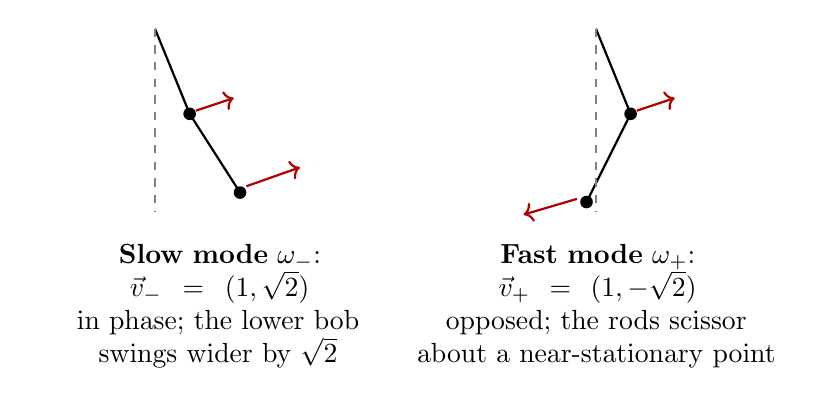
\begin{tikzpicture}[scale=0.8]
  % ---- slow mode: sketch on top, caption below ----
  \draw[thick] (0,0) -- (0.55,-1.35);
  \fill (0.55,-1.35) circle (0.1);
  \draw[thick] (0.55,-1.35) -- (1.35,-2.6);
  \fill (1.35,-2.6) circle (0.1);
  \draw[gray, dashed] (0,0) -- (0,-2.9);
  \draw[->, red!70!black, thick] (0.65,-1.3) -- (1.25,-1.1);
  \draw[->, red!70!black, thick] (1.45,-2.5) -- (2.3,-2.2);
  \node[align=center, text width=4.6cm] at (1.0,-4.4)
    {\textbf{Slow mode} $\omega_-$:\quad $\vec v_- = (1, \sqrt2)$\\
     in phase; the lower bob\\ swings wider by $\sqrt2$};
  % ---- fast mode: sketch on top, caption below ----
  \draw[thick] (7,0) -- (7.55,-1.35);
  \fill (7.55,-1.35) circle (0.1);
  \draw[thick] (7.55,-1.35) -- (6.85,-2.75);
  \fill (6.85,-2.75) circle (0.1);
  \draw[gray, dashed] (7,0) -- (7,-2.9);
  \draw[->, red!70!black, thick] (7.65,-1.3) -- (8.25,-1.1);
  \draw[->, red!70!black, thick] (6.7,-2.7) -- (5.85,-2.95);
  \node[align=center, text width=4.6cm] at (7.0,-4.4)
    {\textbf{Fast mode} $\omega_+$:\quad $\vec v_+ = (1, -\sqrt2)$\\
     opposed; the rods scissor\\ about a near-stationary point};
\end{tikzpicture}
\end{center}

Sanity checks, each one line: the frequencies bracket the single
pendulum's, $\omega_-^2 < g/\ell < \omega_+^2$ (the in-phase mode is
effectively a longer pendulum, the scissoring mode a stiffer one);
$\mM$-orthogonality holds,
$\vec v_-^{\mathsf T}\mM\,\vec v_+ = m\ell^2\,(1,\sqrt2)
\bigl(\begin{smallmatrix}2&1\\1&1\end{smallmatrix}\bigr)
\bigl(\begin{smallmatrix}1\\-\sqrt2\end{smallmatrix}\bigr)
= m\ell^2\,(1,\sqrt2)\cdot(2-\sqrt2,\,1-\sqrt2)^{\mathsf T}
= m\ell^2\bigl(2 - \sqrt2 + \sqrt2 - 2\bigr) = 0$ \checkmark\ (note:
plain orthogonality fails, $(1,\sqrt2)\cdot(1,-\sqrt2) = -1 \ne 0$ ---
the $\mM$-inner product is not decorative); and by
Theorem~\ref{thm:simultaneous}, the general small motion is
\begin{equation}
  \vth(t) = \xi_-(0\text{-data})\,\vec v_-\cos(\omega_- t - \phi_-)
          + \xi_+(0\text{-data})\,\vec v_+\cos(\omega_+ t - \phi_+),
\end{equation}
with beats, energy exchange, and every phenomenon of the oscillator
companion's coupled chapter available on demand.

%=======================================================================
\clearpage
\part{Hamiltonian Mechanics}
%=======================================================================

%=======================================================================
\section{The Legendre Transform and Hamilton's Equations}
%=======================================================================
\label{sec:hamilton}

Lagrangian mechanics runs on $(\vq, \dot\vq)$: positions and velocities.
Hamiltonian mechanics changes one variable --- velocity out, momentum in
--- and before the machinery, the case for bothering. First, the
\emph{shape} of the dynamics changes: $n$ second-order equations become
$2n$ \emph{first-order} ones, so that a single point in the
$2n$-dimensional space of $(\vq,\vp)$ determines the entire future
[existence and uniqueness for the smooth first-order system; stated]
--- the
dynamics becomes a \emph{flow}, and flows can be drawn, transported, and
reasoned about globally (\S\ref{sec:phase-space} will prove a theorem,
Liouville's, that is invisible in the Lagrangian picture and is the
opening axiom of statistical mechanics). Second, the choice of
\emph{momentum} as the fundamental variable is not arbitrary: $p_i$
is what conservation laws conserve (\S\ref{sec:conservation}), and in
quantum mechanics it is $\hat p$, not $\dot{\hat q}$, that stands beside
$\hat q$ in the commutation relations --- classical mechanics in
Hamiltonian form is the version that quantizes. Third, and deepest:
putting $\vq$ and $\vp$ on \emph{equal footing} unlocks a group of
transformations (mixing coordinates with momenta!) vastly larger than the
point transformations of Theorem~\ref{thm:covariance}, and with it the
strongest solution techniques classical mechanics possesses
(\S\ref{sec:outlook}). Goldstein's summary is the standard one: the
Hamiltonian formulation's advantage is not calculational convenience but
structural insight --- it is the formal skeleton on which the more modern
theories of matter are built. The change of variable itself is not a
cosmetic substitution but a \emph{Legendre transform}, whose structure is
worth stating exactly.

\subsection{The transform}
\label{sec:legendre}

\begin{definition}[Legendre transform of the Lagrangian]
\label{def:legendre}
Assume $L(\vq, \dot\vq, t)$ is $C^2$ and \emph{convex in the velocities}:
the Hessian $\bigl(\partial^2 L/\partial\dot q_i\partial\dot q_j\bigr)$ is
positive definite. Define the \emph{canonical momenta}
\begin{equation}
  \boxed{\;p_i \;\equiv\; \pd{L}{\dot q_i}(\vq, \dot\vq, t)\;}
  \label{eq:canonical-momentum}
\end{equation}
Convexity makes the map $\dot\vq \mapsto \vp$ invertible for each fixed
$(\vq, t)$ (its Jacobian is the positive-definite Hessian; the inverse
function theorem applies), so velocities can be re-expressed as
$\dot\vq = \dot\vq(\vq, \vp, t)$. The \emph{Hamiltonian} is
\begin{equation}
  \boxed{\;
  H(\vq, \vp, t)
  \;\equiv\;
  \sum_i p_i\,\dot q_i(\vq,\vp,t) \;-\; L\bigl(\vq, \dot\vq(\vq,\vp,t), t\bigr).
  \;}
  \label{eq:hamiltonian}
\end{equation}
\end{definition}

For mechanical Lagrangians the convexity hypothesis is physical: the
Hessian of $T$ in the velocities is the mass matrix $\mM(\vq)$ of
\S\ref{sec:gevp}, positive definite because kinetic energy is positive.

\subsection{Hamilton's equations by two routes}
\label{sec:hamilton-eqs}

\paragraph{Derivation 1: track the differential.}
Compute $\dd H$ from \eqref{eq:hamiltonian}, treating $H$ as a function of
$(\vq, \vp, t)$ but differentiating through the definition:
\begin{align}
  \dd H
  &= \sum_i \bigl(p_i\,\dd\dot q_i + \dot q_i\,\dd p_i\bigr)
   - \sum_i \pd{L}{q_i}\,\dd q_i
   - \sum_i \underbrace{\pd{L}{\dot q_i}}_{=\,p_i}\,\dd\dot q_i
   - \pd{L}{t}\,\dd t \nonumber\\
  &= \sum_i \dot q_i\,\dd p_i
   \;-\; \sum_i \pd{L}{q_i}\,\dd q_i
   \;-\; \pd{L}{t}\,\dd t .
  \label{eq:dH}
\end{align}
The $\dd\dot q_i$ terms cancel \emph{identically} --- this cancellation is
the entire design of the Legendre transform: it removes the dependence on
the old variable and leaves a function of the new one. Reading off the
coefficients of the independent differentials $\dd q_i, \dd p_i, \dd t$:
\begin{equation}
  \pd{H}{p_i} = \dot q_i,
  \qquad
  \pd{H}{q_i} = -\pd{L}{q_i},
  \qquad
  \pd{H}{t} = -\pd{L}{t} .
  \label{eq:legendre-identities}
\end{equation}
So far, no dynamics --- these are identities of the transform. Dynamics
enters through Euler--Lagrange: \emph{on a solution},
$\partial L/\partial q_i = \tfrac{\dd}{\dd t}(\partial L/\partial\dot q_i)
= \dot p_i$, and the middle identity becomes an equation of motion:
\begin{equation}
  \boxed{\;
  \dot q_i = \pd{H}{p_i},
  \qquad
  \dot p_i = -\,\pd{H}{q_i}
  \;}
  \qquad (i = 1,\dots,n)
  \label{eq:hamilton-eqs}
\end{equation}
--- \emph{Hamilton's equations}: $2n$ \emph{first-order} equations
replacing $n$ second-order ones, in a form so symmetric that
$q$ and $p$ differ only by a sign.

\paragraph{Derivation 2: a variational principle in phase space.}
Hamilton's equations are themselves Euler--Lagrange equations --- of the
\emph{phase-space action}
\begin{equation}
  S[\vq, \vp]
  = \int_{t_0}^{t_1}\Bigl[\sum_i p_i\,\dot q_i - H(\vq,\vp,t)\Bigr]\dd t ,
\end{equation}
in which $\vq(t)$ and $\vp(t)$ are varied \emph{independently}, with the
$q$'s pinned at the endpoints and the $p$'s entirely free. Vary $\vp$
(no integration by parts needed, since $\dot\vp$ never appears):
\begin{equation}
  \delta_p S = \int \sum_i \Bigl[\dot q_i - \pd{H}{p_i}\Bigr]\,
  \delta p_i \,\dd t = 0
  \quad\Longrightarrow\quad
  \dot q_i = \pd{H}{p_i} ,
\end{equation}
by the fundamental lemma. Vary $\vq$ (one integration by parts on
$p_i\,\delta\dot q_i$; the boundary term dies on the pinned $q$'s):
\begin{equation}
  \delta_q S = \int \sum_i\Bigl[-\dot p_i - \pd{H}{q_i}\Bigr]\,
  \delta q_i\,\dd t = 0
  \quad\Longrightarrow\quad
  \dot p_i = -\pd{H}{q_i} .
\end{equation}
Both equations from one functional, on equal footing --- the formulation
that generalizes cleanly (to field theory, and to the path integral).

\paragraph{Energy bookkeeping.}
Along a solution of \eqref{eq:hamilton-eqs},
\begin{equation}
  \frac{\dd H}{\dd t}
  = \sum_i\Bigl[\pd{H}{q_i}\dot q_i + \pd{H}{p_i}\dot p_i\Bigr] + \pd{H}{t}
  = \sum_i\Bigl[\pd{H}{q_i}\pd{H}{p_i} - \pd{H}{p_i}\pd{H}{q_i}\Bigr] + \pd{H}{t}
  \quad\Longrightarrow\quad
  \boxed{\;\frac{\dd H}{\dd t} = \pd{H}{t}\;} :
\end{equation}
\emph{if $H$ has no explicit time dependence it is conserved}.

\begin{remark}[$h$ versus $H$: the same number, not the same function]
\label{rem:h-vs-H}
Comparing \eqref{eq:hamiltonian} with \S\ref{sec:conservation}: along
any state, $H$ takes the \emph{value} of the energy function $h$ ---
$H(\vq, \vp, t) = h(\vq, \dot\vq, t)$ whenever $\vp$ and $\dot\vq$
correspond under \eqref{eq:canonical-momentum}. Are they then the same
object? \emph{No}, and the difference carries the whole formalism: they
are different functions of \emph{different variables} --- $h$ lives on
$(\vq, \dot\vq)$, $H$ on $(\vq, \vp)$ --- and partial derivatives care
about what is held fixed. Concretely, differentiate
$h = \sum_j \dot q_j\,\partial L/\partial\dot q_j - L$ at fixed
$\dot\vq$ and compare with \eqref{eq:legendre-identities}:
\begin{equation}
  \left(\pd{h}{q_i}\right)_{\!\dot\vq}
  = \sum_j \dot q_j\,
    \frac{\partial^2 L}{\partial q_i\,\partial \dot q_j}
  - \pd{L}{q_i},
  \qquad
  \left(\pd{H}{q_i}\right)_{\!\vp}
  = -\,\pd{L}{q_i} :
\end{equation}
the two disagree by
$\sum_j \dot q_j\,\partial^2 L/\partial q_i\partial\dot q_j$ ---
zero for a constant mass matrix, but \emph{nonzero} whenever
$\mM$ depends on the coordinates, as in the double pendulum. This is why
Hamilton's equations hold for $H$ and not for $h$: the clean identity
$\partial H/\partial q_i = -\partial L/\partial q_i$ is a property of
differentiating \emph{at fixed momentum}, and arranging for it is
exactly what the Legendre transform's cancellation in \eqref{eq:dH}
accomplished. The same re-reading applies to the momentum itself:
in \S\ref{sec:conservation}, $p_i = \partial L/\partial\dot q_i$ was a
\emph{derived bookkeeping quantity} --- a combination evaluated along a
trajectory, singled out because cyclic coordinates conserve it. Here the
identical formula is re-read as a \emph{change of variables}, and $p_i$
is promoted to an independent coordinate of state space. Same formula,
different ontological status; the Legendre transform is the promotion
ceremony, and keeping the two names ($h$ on the Lagrangian side, $H$ on
the Hamiltonian side, following Goldstein) keeps the two objects
distinct.
\end{remark}

\begin{remark}[Involutivity]
The transform undoes itself: from \eqref{eq:legendre-identities},
$\dot q_i = \partial H/\partial p_i$, and then
$\sum_i p_i \dot q_i - H = L$ by \eqref{eq:hamiltonian} --- performing the
Legendre transform of $H$ in the $p$'s returns $L$. Lagrangian and
Hamiltonian mechanics are two charts on the same theory, with a
lossless dictionary between them (given convexity).
\end{remark}

\subsection{When is $H = T + V$?}
\label{sec:when-H-is-E}

\begin{proposition}\label{prop:H-is-E}
Suppose the constraints are time-independent (so that
$\vr_a = \vr_a(\vq)$ and $T$ is purely quadratic in the velocities,
$T = \tfrac12\sum_{ij} M_{ij}(\vq)\,\dot q_i\dot q_j$) and $V = V(\vq, t)$
is velocity-independent. Then $H = T + V$.
\end{proposition}
\begin{proof}
The one tool needed is \emph{Euler's theorem on homogeneous functions} in
its quadratic case, proved inline: with
$T = \tfrac12\sum_{ij}M_{ij}\dot q_i\dot q_j$ and $M_{ij}=M_{ji}$,
\begin{equation}
  \pd{T}{\dot q_k} = \sum_j M_{kj}\,\dot q_j
  \quad\Longrightarrow\quad
  \sum_k \dot q_k \pd{T}{\dot q_k}
  = \sum_{kj} M_{kj}\,\dot q_k\dot q_j = 2\,T .
\end{equation}
Since $V$ carries no velocities, $p_k = \partial T/\partial\dot q_k$, and
\begin{equation}
  H = \sum_k p_k\dot q_k - L = 2T - (T - V) = T + V . \qedhere
\end{equation}
\end{proof}

\begin{remark}[The rheonomic caveat]
If the constraints move --- $\vr_a = \vr_a(\vq, t)$, e.g.\ a bead on a
hoop \emph{rotating at imposed rate} --- then $T$ acquires terms linear in
$\dot q$ and a $\dot q$-free term, the computation above breaks, and
$H \ne T + V$. $H$ may still be conserved (if $L$ ends up
$t$-independent) while the mechanical energy $T + V$ is \emph{not} ---
whatever drives the constraint does work. The two statements ``$H$ is
conserved'' and ``$H$ is the energy'' have different hypotheses; conflating
them is the standard trap.
\end{remark}

\subsection{Examples}

\paragraph{Harmonic oscillator.}
$L = \tfrac12 m\dot q^2 - \tfrac12 kq^2$; $p = m\dot q$, so
$\dot q = p/m$ and
\begin{equation}
  H = p\cdot\frac{p}{m} - \frac{p^2}{2m} + \frac12 kq^2
  = \frac{p^2}{2m} + \frac{k q^2}{2},
\end{equation}
\begin{equation}
  \dot q = \pd Hp = \frac pm,
  \qquad
  \dot p = -\pd Hq = -kq
  \quad\Longrightarrow\quad
  \ddot q = \frac{\dot p}{m} = -\frac km q = -\omega_0^2 q .
  \;\checkmark
\end{equation}

The pendulum and the double pendulum deserve more than a paragraph: the
next section re-derives and \emph{completely solves} both in the
Hamiltonian formalism, as the proper stress test of the new machinery.

%=======================================================================
\section{The Two Systems Revisited: Complete Hamiltonian Solutions}
%=======================================================================
\label{sec:revisit}

Part I solved the pendulum and the double pendulum by the Lagrangian
recipe. We now solve both again, start to finish, in the Hamiltonian
formalism --- not as repetition but as calibration: the same physics must
come out, and watching \emph{where the same content sits in the two
formalisms} is how a formalism is actually learned.

\subsection{Complete solution of the pendulum}
\label{sec:pendulum-H}

\paragraph{Setting up.}
From \S\ref{sec:pendulum}, $L = \tfrac12 m\ell^2\dot\theta^2 +
mg\ell\cos\theta$. The canonical momentum and its inversion:
\begin{equation}
  p = \pd{L}{\dot\theta} = m\ell^2\dot\theta
  \qquad\Longleftrightarrow\qquad
  \dot\theta = \frac{p}{m\ell^2}
\end{equation}
--- physically, $p$ is the \emph{angular momentum} about the pivot
(moment of inertia $m\ell^2$ times angular velocity); the canonical
momentum conjugate to an angle is always an angular momentum. The
Hamiltonian, via \eqref{eq:hamiltonian} or directly via
Proposition~\ref{prop:H-is-E} ($T + V$; the constraint is
time-independent):
\begin{equation}
  \boxed{\;
  H(\theta, p) = \frac{p^2}{2m\ell^2} - mg\ell\cos\theta
  \;}
  \label{eq:pendulum-H}
\end{equation}
Hamilton's equations \eqref{eq:hamilton-eqs}:
\begin{equation}
  \dot\theta = \pd{H}{p} = \frac{p}{m\ell^2},
  \qquad
  \dot p = -\pd{H}{\theta} = -\,mg\ell\sin\theta .
  \label{eq:pendulum-hamilton}
\end{equation}
(Consistency: differentiate the first equation and substitute the second
to recover $\ddot\theta = -(g/\ell)\sin\theta$, equation
\eqref{eq:pendulum-eom}. The same physics redistributed: one
second-order
equation has become a pair of first-order ones, and the pair is what
draws the phase portrait of \S\ref{sec:phase-space}.)

\paragraph{Small angles: the complete solution.}
Expand $H$ to quadratic order ($\cos\theta = 1 - \tfrac12\theta^2 +
O(\theta^4)$; drop the constant):
\begin{equation}
  H_2 = \frac{p^2}{2m\ell^2} + \frac{mg\ell}{2}\,\theta^2 ,
  \qquad
  \dot\theta = \frac{p}{m\ell^2},
  \quad
  \dot p = -\,mg\ell\,\theta .
\end{equation}
Differentiating the first equation and inserting the second gives
$\ddot\theta = -(g/\ell)\theta = -\omega_0^2\theta$; then $p$ follows
from $p = m\ell^2\dot\theta$. With initial data $(\theta_0, p_0)$:
\begin{equation}
  \boxed{\;
  \theta(t) = \theta_0\cos\omega_0 t
    + \frac{p_0}{m\ell^2\omega_0}\,\sin\omega_0 t,
  \qquad
  p(t) = p_0\cos\omega_0 t - m\ell^2\omega_0\,\theta_0\sin\omega_0 t
  \;}
  \label{eq:pendulum-full-solution}
\end{equation}
(Checks: at $t=0$ the pair returns $(\theta_0, p_0)$ \checkmark;
substituting both expressions into \eqref{eq:pendulum-hamilton} verifies
the equations at all times, term by term \checkmark.) \emph{Every} small
motion of the pendulum is \eqref{eq:pendulum-full-solution} ---
completeness leans on uniqueness for the linear system, which the
energy method proves in three lines: the difference of two solutions
with the same initial data starts with $H_2 = 0$, keeps $H_2$
conserved, and $H_2$ is positive definite, so the difference vanishes
identically. The problem is closed.

Geometry of the solution: eliminate $t$. Direct substitution (using
$\cos^2 + \sin^2 = 1$) shows
$\tfrac{1}{2m\ell^2}p(t)^2 + \tfrac{mg\ell}{2}\theta(t)^2
= H_2(\theta_0, p_0) \equiv E$ for all $t$, so the orbit is the ellipse
\begin{equation}
  \frac{\theta^2}{2E/mg\ell} + \frac{p^2}{2m\ell^2 E} = 1
\end{equation}
with semi-axes $\sqrt{2E/mg\ell}$ and $\sqrt{2m\ell^2E}$, traversed once
per period --- precisely the small ovals around the centers of
Fig.~\ref{fig:phase-portraits}. Its enclosed area is $\pi$ times the
product of the semi-axes,
\begin{equation}
  \text{area}
  = \pi\sqrt{\frac{2E}{mg\ell}}\,\sqrt{2m\ell^2 E}
  = 2\pi E\sqrt{\frac{\ell}{g}}
  = \frac{2\pi E}{\omega_0}
\end{equation}
--- area $=$ $2\pi\,\times$ energy over frequency. The quantity
$E/\omega_0$ (enclosed area over $2\pi$) is the \emph{action variable} of
Hamilton--Jacobi theory (\S\ref{sec:hj}, Remark~\ref{rem:hj-beyond}),
making its first, unforced appearance.

\paragraph{Large angles: complete reduction to quadrature.}
Beyond small angles the Hamiltonian route still delivers everything short
of elementary functions, in three moves. \emph{(i) Conservation solves
for $p$}: on the energy surface $H = E$,
\begin{equation}
  p(\theta) = \pm\sqrt{2m\ell^2\,\bigl(E + mg\ell\cos\theta\bigr)} .
\end{equation}
\emph{(ii) The first Hamilton equation separates}: from
$\dot\theta = p/m\ell^2$,
\begin{equation}
  t(\theta) = \int \frac{m\ell^2\;\dd\theta}
  {\sqrt{2m\ell^2\bigl(E + mg\ell\cos\theta\bigr)}}
  \label{eq:pendulum-quadrature}
\end{equation}
--- the dynamics is \emph{reduced to quadrature}: one integral stands
between the initial data and the full trajectory. \emph{(iii) The period,
explicitly.} For libration with turning angle $\theta_{\max}$ (where
$p = 0$): $E = -mg\ell\cos\theta_{\max}$, and a quarter period runs from
$\theta = 0$ to $\theta_{\max}$:
\begin{equation}
  \frac{T}{4}
  = \sqrt{\frac{\ell}{2g}} \int_0^{\theta_{\max}}
  \frac{\dd\theta}{\sqrt{\cos\theta - \cos\theta_{\max}}} .
\end{equation}
Convert with $\cos\theta = 1 - 2\sin^2(\theta/2)$, so that
$\cos\theta - \cos\theta_{\max}
= 2\bigl(\sin^2\tfrac{\theta_{\max}}{2} - \sin^2\tfrac{\theta}{2}\bigr)$;
then substitute $\sin\tfrac{\theta}{2} = k\sin\varphi$ with
$k \equiv \sin\tfrac{\theta_{\max}}{2}$ (so $\varphi: 0 \to \pi/2$ as
$\theta: 0 \to \theta_{\max}$), whence
$\tfrac12\cos\tfrac{\theta}{2}\,\dd\theta = k\cos\varphi\,\dd\varphi$ and
$\cos\tfrac{\theta}{2} = \sqrt{1 - k^2\sin^2\varphi}$:
\begin{equation}
  \frac{T}{4}
  = \sqrt{\frac{\ell}{2g}}\int_0^{\pi/2}
  \frac{1}{\sqrt{2}\;\sqrt{1 - k^2\sin^2\varphi}}\cdot
  \frac{2k\cos\varphi\;\dd\varphi}{k\cos\varphi}
  \quad\Longrightarrow\quad
  \boxed{\;
  T = 4\sqrt{\frac{\ell}{g}}\;K\!\Bigl(\sin\tfrac{\theta_{\max}}{2}\Bigr)
  \;}
\end{equation}
--- the elliptic-integral period stated in
Remark~\ref{rem:exact-pendulum}, now derived. Every qualitative feature
of the phase portrait becomes quantitative here: $K(k) \to \pi/2$ as
$k \to 0$ recovers $T = 2\pi\sqrt{\ell/g}$, and $K(k) \to \infty$ as
$k \to 1$ ($\theta_{\max}\to\pi$) is the diverging period at the
separatrix.

\subsection{Complete solution of the double pendulum}
\label{sec:dp-H}

\paragraph{The Hamiltonian for any quadratic kinetic energy.}
One structural proposition organizes everything.

\begin{proposition}\label{prop:matrix-H}
If $L = \tfrac12\,\dot\vq^{\mathsf T}\mM(\vq)\,\dot\vq - V(\vq)$ with
$\mM(\vq)$ symmetric positive definite, then
\begin{equation}
  \vp = \mM(\vq)\,\dot\vq,
  \qquad
  \dot\vq = \mM(\vq)^{-1}\vp,
  \qquad
  \boxed{\;
  H(\vq,\vp) = \tfrac12\,\vp^{\mathsf T}\mM(\vq)^{-1}\,\vp + V(\vq) .
  \;}
\end{equation}
\end{proposition}
\begin{proof}
$p_i = \partial L/\partial\dot q_i = \sum_j M_{ij}\dot q_j$ is
$\vp = \mM\dot\vq$; positive definiteness makes $\mM$ invertible, giving
the middle display. Then, using the symmetry of $\mM^{-1}$,
\begin{equation}
  H = \vp^{\mathsf T}\dot\vq - L
  = \vp^{\mathsf T}\mM^{-1}\vp
  - \tfrac12 (\mM^{-1}\vp)^{\mathsf T}\mM\,(\mM^{-1}\vp) + V
  = \tfrac12\,\vp^{\mathsf T}\mM^{-1}\vp + V .
\end{equation}
(This is Proposition~\ref{prop:H-is-E} again --- $H = T + V$ --- with $T$
now written in the momenta.)
\end{proof}

\paragraph{The exact double-pendulum Hamiltonian.}
From \S\ref{sec:double-pendulum}, with $\Delta = \theta_1 - \theta_2$,
\begin{equation}
  \mM(\vth) =
  \begin{pmatrix}
    (m_1{+}m_2)\ell_1^2 & m_2\ell_1\ell_2\cos\Delta\\[2pt]
    m_2\ell_1\ell_2\cos\Delta & m_2\ell_2^2
  \end{pmatrix},
\end{equation}
whose determinant deserves one display of its own:
\begin{equation}
  \det\mM
  = (m_1{+}m_2)\,m_2\,\ell_1^2\ell_2^2
  - m_2^2\ell_1^2\ell_2^2\cos^2\Delta
  = m_2\,\ell_1^2\ell_2^2\,\bigl(m_1 + m_2\sin^2\Delta\bigr)
  \;>\; 0
\end{equation}
for \emph{all} configurations --- the mass matrix never degenerates (even
with the rods aligned, $\sin\Delta = 0$, the $m_1$ term keeps it
positive), so the Legendre transform is globally legitimate. Inverting
the $2\times2$ matrix and applying Proposition~\ref{prop:matrix-H}:
\begin{equation}
  \boxed{\;
  H = \frac{m_2\ell_2^2\,p_1^2 + (m_1{+}m_2)\ell_1^2\,p_2^2
      - 2m_2\ell_1\ell_2\cos\Delta\;p_1 p_2}
      {2\,m_2\,\ell_1^2\ell_2^2\,\bigl(m_1 + m_2\sin^2\Delta\bigr)}
  \;-\;(m_1{+}m_2)g\ell_1\cos\theta_1 - m_2g\ell_2\cos\theta_2
  \;}
  \label{eq:dp-H-exact}
\end{equation}
with $p_1 = (m_1{+}m_2)\ell_1^2\dot\theta_1 +
m_2\ell_1\ell_2\cos\Delta\,\dot\theta_2$ and
$p_2 = m_2\ell_2^2\dot\theta_2 + m_2\ell_1\ell_2\cos\Delta\,\dot\theta_1$.
The exact dynamics is the four first-order equations
\begin{equation}
  \dot\vth = \mM(\vth)^{-1}\vp,
  \qquad
  \dot\vp = -\,\pd{}{\vth}\Bigl[\tfrac12\vp^{\mathsf T}\mM(\vth)^{-1}\vp\Bigr]
  - \pd{V}{\vth},
\end{equation}
where the configuration-dependence of the inverse is differentiated via
$\partial_\theta\,\mM^{-1} = -\,\mM^{-1}(\partial_\theta\mM)\,\mM^{-1}$
(differentiate $\mM\mM^{-1} = \mathbb{1}$ by the product rule and solve).
These four equations are the complete dynamical content of the system ---
what a numerical integrator integrates, and the flow whose chaos
\S\ref{sec:outlook} describes.

\paragraph{Small angles: decoupling and solving Hamilton's equations.}
Quadratic truncation: in the kinetic term $\vp$ is already first-order
small, so $\mM(\vth)^{-1}$ may be evaluated at equilibrium
($\cos\Delta \to 1$; the correction enters at fourth order), giving the
constant matrix $\mM_0$ of \S\ref{sec:linearization}; the potential
truncates as before. With $\mK$ from \eqref{eq:dp-matrix},
\begin{equation}
  H_2 = \tfrac12\,\vp^{\mathsf T}\mM_0^{-1}\vp
  + \tfrac12\,\vth^{\mathsf T}\mK\,\vth,
  \qquad
  \dot\vth = \mM_0^{-1}\vp,
  \quad
  \dot\vp = -\,\mK\vth .
  \label{eq:dp-hamilton-linear}
\end{equation}
Now the payoff of Theorem~\ref{thm:simultaneous}. Take the generalized
eigenvectors $\mK\vec v_r = \omega_r^2\mM_0\vec v_r$, normalized to
$\vec v_r^{\mathsf T}\mM_0\vec v_s = \delta_{rs}$, and define \emph{mode
coordinates and mode momenta}
\begin{equation}
  \xi_r \equiv \vec v_r^{\mathsf T}\,\mM_0\,\vth,
  \qquad
  \pi_r \equiv \vec v_r^{\mathsf T}\,\vp .
\end{equation}
Differentiate each along the flow \eqref{eq:dp-hamilton-linear}:
\begin{align}
  \dot\xi_r &= \vec v_r^{\mathsf T}\mM_0\,\dot\vth
  = \vec v_r^{\mathsf T}\mM_0\,\mM_0^{-1}\vp
  = \vec v_r^{\mathsf T}\vp = \pi_r ,\\
  \dot\pi_r &= \vec v_r^{\mathsf T}\dot\vp
  = -\,\vec v_r^{\mathsf T}\mK\,\vth
  = -\sum_s \xi_s\,\vec v_r^{\mathsf T}\mK\vec v_s
  = -\,\omega_r^2\,\xi_r
\end{align}
(the last step expands $\vth = \sum_s \xi_s\vec v_s$ --- valid because
the $\vec v_s$ are a basis with coefficients recovered by
$\mM_0$-orthonormality --- and uses
$\vec v_r^{\mathsf T}\mK\vec v_s = \omega_s^2\,\vec
v_r^{\mathsf T}\mM_0\vec v_s = \omega_s^2\delta_{rs}$). Each pair obeys
\begin{equation}
  \dot\xi_r = \pi_r,
  \qquad
  \dot\pi_r = -\,\omega_r^2\,\xi_r
\end{equation}
--- Hamilton's equations of the unit-mass oscillator Hamiltonian
$\tfrac12\pi_r^2 + \tfrac12\omega_r^2\xi_r^2$; and indeed substituting
the expansions into $H_2$ collapses it (same two identities) to
\begin{equation}
  \boxed{\;
  H_2 = \sum_{r}\Bigl[\tfrac12\,\pi_r^2
  + \tfrac12\,\omega_r^2\,\xi_r^2\Bigr]
  \;}
\end{equation}
--- \emph{two independent oscillators, additively}. Where the Lagrangian
treatment decoupled the \emph{equations}
(Theorem~\ref{thm:simultaneous}), the Hamiltonian treatment decouples the
\emph{energy itself}: the modes carry separately conserved
energies ($\dot H_r = 0$ each, by the one-oscillator computation). That
the change of variables $(\vth,\vp) \to (\xi,\pi)$ preserves the
Hamiltonian form of the equations makes it our first nontrivial
\emph{canonical transformation}; \S\ref{sec:poisson} will supply the
certificate that verifies this in one line.

\paragraph{The complete general solution.}
Each mode is solved by \eqref{eq:pendulum-full-solution} with
$m\ell^2 \to 1$, $\omega_0 \to \omega_r$:
\begin{equation}
  \xi_r(t) = \xi_r(0)\cos\omega_r t
  + \frac{\pi_r(0)}{\omega_r}\sin\omega_r t ,
  \qquad
  \pi_r(t) = \pi_r(0)\cos\omega_r t - \omega_r\,\xi_r(0)\sin\omega_r t ,
\end{equation}
and translating back through the definitions (using
$\vp(0) = \mM_0\dot\vth(0)$, so $\pi_r(0) = \vec
v_r^{\mathsf T}\mM_0\dot\vth(0)$),
\begin{equation}
  \boxed{\;
  \vth(t) = \sum_{r}
  \Bigl[\bigl(\vec v_r^{\mathsf T}\mM_0\,\vth(0)\bigr)\cos\omega_r t
  + \frac{\vec v_r^{\mathsf T}\mM_0\,\dot\vth(0)}{\omega_r}
  \sin\omega_r t\Bigr]\,\vec v_r
  \;}
  \label{eq:dp-general-solution}
\end{equation}
Four numbers in, one motion out. For equal
masses and lengths everything is explicit:
$\omega_\mp^2 = (2\mp\sqrt2)\,g/\ell$, unnormalized modes
$(1, \pm\sqrt2)$, with $\mM_0$-norms
\begin{equation}
  (1,\ \sqrt2)\,\mM_0\begin{pmatrix}1\\ \sqrt2\end{pmatrix}
  = m\ell^2\bigl(4 + 2\sqrt2\bigr),
  \qquad
  (1,\ -\sqrt2)\,\mM_0\begin{pmatrix}1\\ -\sqrt2\end{pmatrix}
  = m\ell^2\bigl(4 - 2\sqrt2\bigr),
\end{equation}
so $\vec v_\mp = (1, \pm\sqrt2)\big/\sqrt{m\ell^2(4\pm2\sqrt2)}$ in
\eqref{eq:dp-general-solution}. One concrete instance, fully evaluated:
release from rest with the upper rod displaced, $\vth(0) = (\alpha, 0)$,
$\dot\vth(0) = 0$. The mode amplitudes are
$\vec v_\mp^{\mathsf T}\mM_0\vth(0)$ with
$\mM_0\vth(0) = \alpha\,m\ell^2\,(2, 1)^{\mathsf T}$, and assembling
\eqref{eq:dp-general-solution} (all $m\ell^2$ factors cancel between the
amplitude and the normalized eigenvector):
\begin{equation}
  \theta_1(t) = \frac{\alpha}{2}\Bigl[
  \cos\omega_- t + \cos\omega_+ t\Bigr],
  \qquad
  \theta_2(t) = \frac{\alpha}{\sqrt2}\,\Bigl[
  \cos\omega_- t - \cos\omega_+ t\Bigr]
  \label{eq:dp-concrete}
\end{equation}
(equivalently: expanding the initial condition in the eigenbasis,
$(\alpha, 0) = \tfrac\alpha2(1,\sqrt2) + \tfrac\alpha2(1,-\sqrt2)$,
each mode released from rest evolves with its own cosine). Checks:
$\theta_1(0) = \alpha$ \checkmark; $\theta_2(0) = 0$ \checkmark; both
initial velocities vanish since every term is a cosine \checkmark; and
the initial \emph{accelerations} --- the check sensitive to the mode
weights --- match Newton: differentiating twice at $t = 0$ gives
$\ddot\vth(0) = \bigl(-\tfrac\alpha2(\omega_-^2 + \omega_+^2),\,
-\tfrac\alpha{\sqrt2}(\omega_-^2 - \omega_+^2)\bigr)
= \bigl(-2\alpha g/\ell,\, +2\alpha g/\ell\bigr)$, in agreement with
$\ddot\vth(0) = -\mM_0^{-1}\mK\,\vth(0)$ evaluated directly
\checkmark. The lower bob
\eqref{eq:dp-concrete} is a difference of cosines at frequency ratio
$\omega_+/\omega_- = \sqrt{(2{+}\sqrt2)/(2{-}\sqrt2)} = 1 + \sqrt2$ ---
irrational: by the product identity of the oscillator companion the
motion beats, energy migrating between the bobs, and because the ratio is
irrational the motion never exactly repeats. Complete, explicit,
checkable: the Hamiltonian route closes on the same physics the
Lagrangian one opened.

%=======================================================================
\section{Poisson Brackets}
%=======================================================================
\label{sec:poisson}

Hamilton's equations treat $\vq$ and $\vp$ symmetrically; the Poisson
bracket is the algebraic structure that makes the symmetry total. The
motivation is threefold: it packages the dynamics of \emph{every}
observable in one formula (not just coordinates and momenta); it converts
questions about conservation into questions of pure algebra; and it
supplies the practical certificate for \emph{canonical} changes of
variables --- the one promised in \S\ref{sec:dp-H}. It is also, nearly
symbol for symbol, the classical face of the quantum commutator.

\subsection{Definition and algebra}

\begin{definition}
For $C^1$ functions $f, g$ on phase space (possibly time-dependent),
\begin{equation}
  \boxed{\;
  \{f, g\}
  \;\equiv\;
  \sum_{i=1}^n\left(\pd{f}{q_i}\pd{g}{p_i} - \pd{f}{p_i}\pd{g}{q_i}\right).
  \;}
\end{equation}
\end{definition}

Three properties are immediate from the definition, one is not:
\begin{enumerate}
  \item \emph{Bilinearity}: $\{af + bg, h\} = a\{f,h\} + b\{g,h\}$
  ($a,b$ constants) --- derivatives are linear.
  \item \emph{Antisymmetry}: $\{f,g\} = -\{g,f\}$; in particular
  $\{f,f\}=0$ --- swap the two terms.
  \item \emph{Leibniz rule}: $\{fg, h\} = f\{g,h\} + \{f,h\}\,g$ --- apply
  the product rule inside each partial derivative of $fg$ and regroup:
  $\partial_i(fg) = f\,\partial_i g + (\partial_i f)\,g$ in both slots.
  The bracket with $h$ acts as a \emph{derivation}.
  \item \emph{Jacobi identity}:
  \begin{equation}
    \boxed{\;
    \{f, \{g,h\}\} + \{g, \{h,f\}\} + \{h, \{f,g\}\} = 0 .
    \;}
  \end{equation}
  Not obvious: each summand contains second derivatives, and the identity
  asserts a threefold cancellation. The full computation is
  Appendix~\ref{app:jacobi}; the organizing idea (worth knowing) is to
  sort all terms by \emph{which} function carries the second derivative
  and check that each of the three groups cancels internally, using only
  the symmetry of mixed partials.
\end{enumerate}

The canonical variables themselves obey the \emph{fundamental brackets}
(direct evaluation: $\partial q_i/\partial q_j = \delta_{ij}$ etc.):
\begin{equation}
  \{q_i, q_j\} = 0,
  \qquad
  \{p_i, p_j\} = 0,
  \qquad
  \boxed{\;\{q_i, p_j\} = \delta_{ij}\;}
\end{equation}

\begin{example}[The certificate promised in \S\ref{sec:dp-H}]
\label{ex:mode-canonical}
A change of variables is \emph{canonical} --- preserves the Hamiltonian
form of the equations for every $H$ --- precisely when the new variables
reproduce the fundamental brackets (we use the criterion here in advance;
\S\ref{sec:hj-ct} states and proves it in the direction this example
needs). For the mode variables of the double pendulum,
$\xi_r = \vec v_r^{\mathsf T}\mM_0\vth$,
$\pi_r = \vec v_r^{\mathsf T}\vp$:
\begin{equation}
  \{\xi_r, \pi_s\}
  = \sum_i \left[\pd{\xi_r}{\theta_i}\pd{\pi_s}{p_i}
  - \underbrace{\pd{\xi_r}{p_i}}_{=\,0}\pd{\pi_s}{\theta_i}\right]
  = \sum_i (\mM_0\vec v_r)_i\,(\vec v_s)_i
  = \vec v_s^{\mathsf T}\mM_0\,\vec v_r
  = \delta_{rs} ,
\end{equation}
and $\{\xi_r,\xi_s\} = \{\pi_r,\pi_s\} = 0$ similarly (each
variable of a pair depends on only one half of the phase-space
coordinates). The $\mM_0$-orthonormality of the modes --- which entered
\S\ref{sec:gevp} as linear algebra --- is revealed as exactly the
condition that mode variables are canonical.
\end{example}

\subsection{Dynamics as bracket flow}

\begin{proposition}\label{prop:bracket-flow}
Along any solution of Hamilton's equations, every $C^1$ phase-space
function $f(\vq,\vp,t)$ evolves by
\begin{equation}
  \boxed{\;
  \frac{\dd f}{\dd t} = \{f, H\} + \pd{f}{t} .
  \;}
\end{equation}
\end{proposition}
\begin{proof}
Chain rule along the trajectory, then Hamilton's equations
\eqref{eq:hamilton-eqs}:
\begin{equation}
  \frac{\dd f}{\dd t}
  = \sum_i\Bigl[\pd{f}{q_i}\dot q_i + \pd{f}{p_i}\dot p_i\Bigr] + \pd{f}{t}
  = \sum_i\Bigl[\pd{f}{q_i}\pd{H}{p_i} - \pd{f}{p_i}\pd{H}{q_i}\Bigr]
  + \pd{f}{t}
  = \{f,H\} + \pd{f}{t} . \qedhere
\end{equation}
\end{proof}

Special cases assemble the whole formalism into one notation: taking
$f = q_i$ and $f = p_i$ recovers Hamilton's equations themselves,
\begin{equation}
  \dot q_i = \{q_i, H\},
  \qquad
  \dot p_i = \{p_i, H\}
\end{equation}
--- coordinates and momenta on \emph{identical} footing; taking $f = H$
recovers $\dd H/\dd t = \partial H/\partial t$ (antisymmetry kills
$\{H,H\}$); and conservation acquires its final form:
\begin{equation}
  f \text{ (time-independent) is conserved}
  \quad\Longleftrightarrow\quad
  \{f, H\} = 0 .
\end{equation}

\begin{corollary}[Poisson's theorem]\label{cor:poisson-thm}
If $f$ and $g$ are conserved (time-independent, $\{f,H\} = \{g,H\} = 0$),
so is $\{f, g\}$.
\end{corollary}
\begin{proof}
By Jacobi with $h = H$:
$\{\{f,g\}, H\} = -\{\{g,H\},f\} - \{\{H,f\},g\} = -\{0,f\} - \{0,g\} = 0$
(after shuffling with antisymmetry). New conserved quantities from old,
by pure algebra --- occasionally the bracket closes on the old ones
(angular momenta: $\{L_x, L_y\} = L_z$), occasionally it produces
genuinely new information.
\end{proof}

\subsection{Noether revisited: conserved quantities generate their symmetries}
\label{sec:noether-hamiltonian}

Noether's theorem (\S\ref{sec:conservation}) was a one-way street:
symmetry in, conserved quantity out. The Hamiltonian formalism reveals
the street runs both ways --- and that the two directions are the
\emph{same equation}.

The key construction: any time-independent phase-space function
$G(\vq,\vp)$ can be installed in place of $H$ and used to generate a
\emph{flow} --- a one-parameter family of transformations obtained by
solving Hamilton's equations with $G$ as the generator,
\begin{equation}
  \frac{\dd q_i}{\dd s} = \pd{G}{p_i},
  \qquad
  \frac{\dd p_i}{\dd s} = -\pd{G}{q_i}
  \qquad
  \Bigl(\text{so that } \frac{\dd f}{\dd s} = \{f, G\}
  \text{ for any } f\Bigr).
\end{equation}
Time evolution is then just the special case $G = H$, $s = t$. Now read
one bracket in two directions:
\begin{equation}
  \boxed{\;
  \underbrace{\{G, H\} = 0}_{\text{$G$ conserved under time evolution}}
  \quad\Longleftrightarrow\quad
  \underbrace{\{H, G\} = 0}_{\text{$H$ invariant under the flow of $G$}}
  \;}
\end{equation}
--- the equivalence is the antisymmetry of the bracket, nothing more.
\emph{A quantity is conserved precisely when the transformation it
generates is a symmetry of the Hamiltonian.} Symmetry and conservation,
which Noether's theorem related by a computation, are exposed as one
relation viewed from its two ends.

The circle closes on \S\ref{sec:conservation} exactly: given a point
symmetry with generator $\eta_i(\vq)$, Noether's conserved quantity was
$I = \sum_i p_i\,\eta_i(\vq)$ --- and the flow that \emph{this} $I$
generates is
\begin{equation}
  \frac{\dd q_i}{\dd s} = \pd{I}{p_i} = \eta_i(\vq) ,
\end{equation}
the original symmetry transformation itself. Check two instances:
\begin{itemize}
  \item $G = p$ (one degree of freedom): flow
  $\dd q/\dd s = 1$, $\dd p/\dd s = 0$, i.e.\ $q \mapsto q + s$ ---
  \emph{momentum generates translations}.
  \item $G = L_z = x p_y - y p_x$: flow
  $\dd x/\dd s = \partial L_z/\partial p_x = -y$,
  $\dd y/\dd s = \partial L_z/\partial p_y = x$ --- the infinitesimal
  rotation, with generator $(-y, x)$ matching the $\eta$ of the Noether
  example in \S\ref{sec:conservation} --- \emph{angular momentum
  generates rotations}.
\end{itemize}
This is why conservation laws are placed where they are in this document:
the theorem and its proof live on the Lagrangian side, where symmetries
of $L$ are stated; but their deepest formulation --- observables as
generators, symmetry $\Leftrightarrow$ conservation as a single
antisymmetric bracket --- is Hamiltonian property, and it is the form
that survives into quantum mechanics ($\hat p$ generates translations,
$\hat L_z$ generates rotations, $\hat H$ generates time evolution).

\begin{remark}[The structure that survives quantization]
The triple (bilinear, antisymmetric, Jacobi) makes phase-space functions
a \emph{Lie algebra}, with the Leibniz rule tying the algebra to the
geometry. Quantum mechanics keeps this entire structure and changes one
thing: $\{f,g\} \to \tfrac{1}{\ii\hbar}[\hat f, \hat g]$. In particular
$\{q,p\} = 1$ becomes $[\hat q, \hat p] = \ii\hbar$. The bracket is not a
notational convenience; it is the load-bearing wall.
\end{remark}

%=======================================================================
\section{Phase Space}
%=======================================================================
\label{sec:phase-space}

\subsection{Portraits}

The state of the system is the point $(\vq, \vp)$; Hamilton's equations
define a \emph{flow} on this $2n$-dimensional space, and for one degree of
freedom the entire global behavior can be drawn: since $H$ is conserved,
\emph{trajectories are level curves of $H$}, and drawing dynamics reduces
to drawing contour lines.

\begin{figure}[ht]
  \centering
  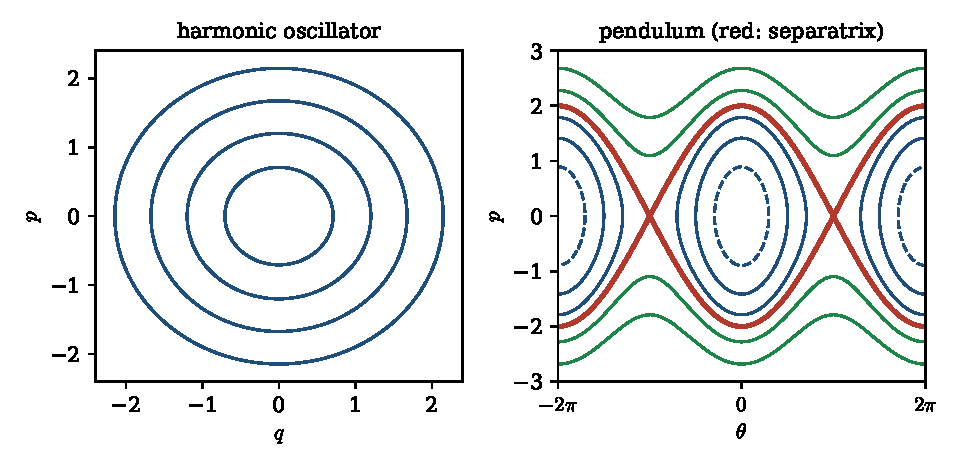
\includegraphics[width=0.95\textwidth]{fig_phase_portraits.pdf}
  \caption{Left: the oscillator, $H = p^2/2m + kq^2/2$ --- nested
  ellipses, one period each. Right: the pendulum
  \eqref{eq:pendulum-H} in normalized variables --- closed curves
  (libration) inside the red \emph{separatrix}, wavy open curves
  (rotation) outside it.}
  \label{fig:phase-portraits}
\end{figure}

Read the pendulum portrait as a summary of everything the system can do:
\begin{itemize}
  \item \textbf{Centers}: $(\theta, p) = (0, 0)$ (and its $2\pi$
  translates) are stable equilibria; nearby level curves are small
  ellipses --- the small-angle oscillator of \S\ref{sec:pendulum},
  literally visible as the elliptical shape of low-energy contours.
  \item \textbf{Saddle}: $(\pm\pi, 0)$, the inverted pendulum, is an
  unstable equilibrium; level curves near it form an X.
  \item \textbf{Separatrix} (red): the level set $H = +mg\ell$ through the
  saddles --- the watershed between \emph{libration} (back-and-forth,
  closed curves) and \emph{rotation} (over the top, open curves). A motion
  \emph{on} the separatrix approaches the inverted position forever
  without arriving; the period of libration diverges as the amplitude
  approaches $\pi$ (the elliptic $K$ of
  Remark~\ref{rem:exact-pendulum} blowing up as $k \to 1$).
\end{itemize}
One conserved function, one picture, the full qualitative theory --- the
economy that makes the Hamiltonian viewpoint the natural language for
global and long-time questions.

\subsection{Liouville's theorem}
\label{sec:liouville}

The flow does not merely move points; it moves them
\emph{incompressibly}.

\begin{theorem}[Liouville]\label{thm:liouville}
The Hamiltonian phase flow preserves phase-space volume: if a region
$\Omega_0$ of initial conditions is carried by the flow to $\Omega_t$,
then $\mathrm{vol}(\Omega_t) = \mathrm{vol}(\Omega_0)$.
\end{theorem}

\begin{proof}
The flow is generated by the phase-space velocity field
\begin{equation}
  X = \bigl(\dot q_1,\dots,\dot q_n,\;\dot p_1,\dots,\dot p_n\bigr)
    = \Bigl(\pd{H}{p_1},\dots,\pd{H}{p_n},\;
      -\pd{H}{q_1},\dots,-\pd{H}{q_n}\Bigr).
\end{equation}
Its divergence vanishes \emph{identically}:
\begin{equation}
  \nabla\cdot X
  = \sum_{i=1}^n\left[\pd{}{q_i}\pd{H}{p_i}
  + \pd{}{p_i}\Bigl(-\pd{H}{q_i}\Bigr)\right]
  = \sum_{i=1}^n\left[\frac{\partial^2 H}{\partial q_i\,\partial p_i}
  - \frac{\partial^2 H}{\partial p_i\,\partial q_i}\right]
  = 0
\end{equation}
by equality of mixed partials ($H \in C^2$) --- note the mechanism: the
\emph{minus sign} in Hamilton's equations pairs each expansion rate
$\partial\dot q_i/\partial q_i$ with an equal and opposite contraction
rate $\partial\dot p_i/\partial p_i$. For a region advected by a flow, the
rate of change of volume is the flux of the velocity field through its
boundary [the transport identity; stated --- it is the
change-of-variables formula for the flow map, differentiated at $t$],
which by the divergence theorem is the integral of the
divergence:
\begin{equation}
  \frac{\dd}{\dd t}\,\mathrm{vol}(\Omega_t)
  = \oint_{\partial\Omega_t} X\cdot\vec n\;\dd A
  = \int_{\Omega_t} \nabla\cdot X\;\dd V
  = 0 . \qedhere
\end{equation}
\end{proof}

\begin{remark}[What Liouville forbids and what breaks it]
Volume preservation forbids \emph{attractors}: no open set of initial
conditions in a Hamiltonian system can funnel into a point or a small
cycle, because its volume would have to shrink. Contrast the damped
oscillator of the companion document: adding $-b\dot q$ makes
$\dot p = -kq - \tfrac{b}{m}p$, the divergence becomes $-b/m < 0$, and
every region contracts exponentially onto the rest point --- dissipation
is, precisely, the failure of Liouville. The theorem is also the opening
axiom of statistical mechanics: it is what allows a probability density on
phase space to be transported like an incompressible fluid.
\end{remark}

%=======================================================================
\section{Canonical Transformations and Hamilton--Jacobi Theory}
%=======================================================================
\label{sec:hj}

The story of this document has been a story about changes of variables.
Theorem~\ref{thm:covariance} established that the Lagrangian framework
survives \emph{any} smooth invertible change of the coordinates $\vq$;
normal coordinates (\S\ref{sec:dp-explicit}) showed how much a good
choice delivers --- the double pendulum fell apart into two clocks. But the
Hamiltonian framework has twice as many variables, and
\S\ref{sec:poisson} already met a change of variables that mixes them:
the mode variables $(\xi_r, \pi_r)$ of
Example~\ref{ex:mode-canonical} are built from the $\theta$'s alone,
but nothing in the bracket criterion required that. This section asks
the question that example left open --- \emph{which} transformations of
phase space preserve Hamiltonian mechanics --- proves the criterion the
example used, and then pushes the freedom to its logical end: a
transformation so well adapted that the new Hamiltonian is \emph{zero}
and the new variables do not move at all. The condition for its
generating function is a single partial differential equation, the
\emph{Hamilton--Jacobi equation}, and the function that satisfies it
turns out to be an old acquaintance: the action itself.

%-----------------------------------------------------------------------
\subsection{Canonical transformations}
\label{sec:hj-ct}

Consider a smooth, invertible, possibly time-dependent change of
phase-space variables
\begin{equation}
  Q_i = Q_i(\vq, \vp, t), \qquad
  P_i = P_i(\vq, \vp, t), \qquad i = 1, \dots, n .
  \label{eq:ct-map}
\end{equation}

\begin{definition}[Canonical transformation]
\label{def:canonical}
The transformation \eqref{eq:ct-map} is \emph{canonical} if for every
Hamiltonian $H(\vq, \vp, t)$ there exists a function $K(\vQ, \vP, t)$
such that curves satisfying Hamilton's equations for $(\vq, \vp; H)$
are carried exactly to curves satisfying Hamilton's equations for
$(\vQ, \vP; K)$:
\begin{equation}
  \dot Q_i = \pd{K}{P_i}, \qquad \dot P_i = -\pd{K}{Q_i} .
\end{equation}
\end{definition}

The demand ``for every $H$'' is what gives the notion teeth: we are
classifying changes of variables that respect the \emph{form} of the
theory, not tricks adapted to one system --- the same standard
Theorem~\ref{thm:covariance} set on the Lagrangian side.

Two examples calibrate how large the class is. First, every point
transformation $\vQ = \vQ(\vq, t)$ extends to a canonical
transformation (with $P$ built from the covariant transformation of
momenta); this is Theorem~\ref{thm:covariance} read through the
Legendre transform, and we will recover it from the generating-function
machinery below. Second --- and this is what point transformations can
never do --- the swap
\begin{equation}
  Q = p, \qquad P = -q
  \label{eq:ct-swap}
\end{equation}
is canonical. Check it in full for one degree of freedom: define
$K(Q, P, t) \equiv H(q, p, t)$, i.e.\ $K(Q,P,t) = H(-P, Q, t)$. Then
along a solution of the old equations,
\begin{equation}
  \dot Q = \dot p = -\pd{H}{q}
  = -\pd{H}{q}(-P, Q, t)
  = \pd{K}{P},
  \qquad
  \dot P = -\dot q = -\pd{H}{p}
  = -\pd{K}{Q} ,
\end{equation}
where the middle steps used the chain rule on $K(Q,P,t) = H(-P,Q,t)$:
$\partial K/\partial P = \partial H/\partial q \cdot (-1)$ and
$\partial K/\partial Q = \partial H/\partial p$. The new equations hold
with the \emph{same} Hamiltonian, relabeled. Coordinates and momenta
are not two kinds of object in this formalism; they are two halves of
one state, exchangeable at the cost of a sign --- the symmetry that
Hamilton's equations \eqref{eq:hamilton-eqs} wear on their face.

\paragraph{The bracket criterion, now proved.}
Example~\ref{ex:mode-canonical} used, without proof, the statement
that a time-independent transformation is canonical precisely when it
reproduces the fundamental brackets. Here is the proof, in the
direction the example needed.

\begin{proposition}[Fundamental brackets $\Rightarrow$ canonical;
time-independent case]
\label{prop:bracket-canonical}
Let $Q_i(\vq,\vp)$, $P_i(\vq,\vp)$ be a smooth invertible
time-independent transformation satisfying
\begin{equation}
  \{Q_i, Q_j\} = 0, \qquad
  \{P_i, P_j\} = 0, \qquad
  \{Q_i, P_j\} = \delta_{ij}
  \qquad (\text{all brackets in } \vq, \vp).
  \label{eq:fundamental-brackets}
\end{equation}
Then the transformation is canonical with $K(\vQ, \vP, t)$ defined by
substitution, $K(\vQ(\vq,\vp), \vP(\vq,\vp), t) = H(\vq, \vp, t)$.
\end{proposition}

\begin{proof}
The engine is Proposition~\ref{prop:bracket-flow}: along any solution,
$\dot F = \{F, H\}$ for every phase-space function $F$ (with no
$\partial F/\partial t$ term here, since $Q_i, P_i$ are
time-independent). Apply it to $F = Q_i$:
\begin{equation}
  \dot Q_i = \{Q_i, H\} .
\end{equation}
Now express $H$ through the new variables, $H = K(\vQ(\vq,\vp),
\vP(\vq,\vp), t)$, and expand the bracket by the chain rule. Writing it
out from the definition --- no shortcut, since this is the step that
carries the proof:
\begin{align}
  \{Q_i, H\}
  &= \sum_{a=1}^{n}\Bigl[
      \pd{Q_i}{q_a}\,\pd{H}{p_a}
    - \pd{Q_i}{p_a}\,\pd{H}{q_a}
    \Bigr] \nonumber\\
  &= \sum_{a=1}^{n}\Biggl[
      \pd{Q_i}{q_a}
      \sum_{j=1}^{n}\Bigl(\pd{K}{Q_j}\pd{Q_j}{p_a}
                        + \pd{K}{P_j}\pd{P_j}{p_a}\Bigr)
    - \pd{Q_i}{p_a}
      \sum_{j=1}^{n}\Bigl(\pd{K}{Q_j}\pd{Q_j}{q_a}
                        + \pd{K}{P_j}\pd{P_j}{q_a}\Bigr)
    \Biggr] \nonumber\\
  &= \sum_{j=1}^{n}\pd{K}{Q_j}
     \underbrace{\sum_{a=1}^{n}\Bigl[
       \pd{Q_i}{q_a}\pd{Q_j}{p_a} - \pd{Q_i}{p_a}\pd{Q_j}{q_a}
     \Bigr]}_{=\;\{Q_i,\,Q_j\}}
   + \sum_{j=1}^{n}\pd{K}{P_j}
     \underbrace{\sum_{a=1}^{n}\Bigl[
       \pd{Q_i}{q_a}\pd{P_j}{p_a} - \pd{Q_i}{p_a}\pd{P_j}{q_a}
     \Bigr]}_{=\;\{Q_i,\,P_j\}} .
  \label{eq:bracket-chain}
\end{align}
The first line is the definition of the bracket; the second applies the
ordinary chain rule to $\partial H/\partial p_a$ and
$\partial H/\partial q_a$; the third merely regroups the four resulting
double sums by which derivative of $K$ they carry --- and the
coefficients that emerge are exactly the fundamental brackets. By
hypothesis \eqref{eq:fundamental-brackets},
\begin{equation}
  \dot Q_i = \sum_j \pd{K}{Q_j}\cdot 0 + \sum_j \pd{K}{P_j}\,\delta_{ij}
  = \pd{K}{P_i} .
\end{equation}
The identical computation with $F = P_i$ gives
\begin{equation}
  \dot P_i = \{P_i, H\}
  = \sum_j \pd{K}{Q_j}\,\{P_i, Q_j\} + \sum_j \pd{K}{P_j}\,\{P_i, P_j\}
  = \sum_j \pd{K}{Q_j}\,(-\delta_{ij})
  = -\pd{K}{Q_i} ,
\end{equation}
using antisymmetry, $\{P_i, Q_j\} = -\{Q_j, P_i\} = -\delta_{ij}$.
Both Hamilton equations hold in the new variables, for arbitrary $H$.
\end{proof}

This closes the loop opened by Example~\ref{ex:mode-canonical}: the mode
variables of the double pendulum, certified there by their brackets,
are now certified canonical by proof. Time-\emph{dependent}
transformations need one more idea --- the new Hamiltonian acquires a
correction term, $K \ne H$ in general --- and that idea is the
generating function.

%-----------------------------------------------------------------------
\subsection{Generating functions}
\label{sec:hj-gen}

The bracket criterion certifies a transformation after the fact. To
\emph{manufacture} canonical transformations --- and eventually to
search for the best one --- we need a handle that produces them. The
handle comes from the variational principle of \S\ref{sec:hamilton-eqs},
Derivation~2: Hamilton's equations for $(\vq, \vp; H)$ say exactly that
the phase-space action
\begin{equation}
  S[\vq, \vp] = \int_{t_0}^{t_1}
  \Bigl[\sum_i p_i\,\dot q_i - H(\vq, \vp, t)\Bigr]\dd t
  \label{eq:ps-action-recall}
\end{equation}
is stationary. Two integrands that differ by a total time derivative
have the same interior variational content --- so if the old and new
integrands differ by one, the two sets of Hamilton equations must
select the same curves. Making this precise is the next proposition;
the care it takes is instructive.

\begin{proposition}[Equivalence up to a total derivative]
\label{prop:total-derivative}
Let \eqref{eq:ct-map} be a smooth invertible transformation, and
suppose there exist smooth functions $K(\vQ,\vP,t)$ and $F$ (of the
phase-space variables and $t$) such that along \emph{every} smooth
phase-space curve,
\begin{equation}
  \sum_i p_i\,\dot q_i - H
  \;=\;
  \sum_i P_i\,\dot Q_i - K
  \;+\; \tot{F}{t} .
  \label{eq:one-form-identity}
\end{equation}
Then a curve satisfies Hamilton's equations for $(\vq, \vp; H)$ if and
only if its image satisfies Hamilton's equations for $(\vQ, \vP; K)$.
\end{proposition}

\begin{proof}
Integrate \eqref{eq:one-form-identity} along any curve from $t_0$ to
$t_1$:
\begin{equation}
  S[\vq, \vp]
  = S'[\vQ, \vP] + F\big|_{t_1} - F\big|_{t_0},
  \label{eq:action-difference}
\end{equation}
where $S'$ is the phase-space action built from $(\vQ, \vP; K)$. Now
restrict attention to \emph{compactly supported} variations: variations
$(\delta\vq, \delta\vp)$ that vanish identically on neighborhoods of
$t_0$ and $t_1$ (the bump functions of
Appendix~\ref{app:fundamental-lemma} are of exactly this kind). Three
observations, each doing one job:

\emph{(i) The boundary term drops out.} A compactly supported variation
leaves the curve unchanged near the endpoints, so $F|_{t_0}$ and
$F|_{t_1}$ --- functions of the curve's endpoint data --- are unvaried.
Varying \eqref{eq:action-difference},
\begin{equation}
  \delta S = \delta S'
  \qquad \text{(compactly supported variations)} .
  \label{eq:deltaS-equal}
\end{equation}

\emph{(ii) Compact support is preserved by the transformation.} Since
\eqref{eq:ct-map} is smooth and invertible, a variation of
$(\vq, \vp)$ vanishing near the endpoints induces a variation of
$(\vQ, \vP)$ vanishing near the endpoints, and conversely. So
``compactly supported'' means the same thing on both sides of
\eqref{eq:deltaS-equal}.

\emph{(iii) Stationarity under compactly supported variations is
exactly Hamilton's equations.} Rerun Derivation~2 of
\S\ref{sec:hamilton-eqs} with compactly supported variations: the
$\vp$-variation needs no boundary condition at all, and the
$\vq$-variation's single integration by parts produces a boundary term
$[\,p_i\,\delta q_i\,]_{t_0}^{t_1}$ that vanishes because
$\delta q_i$ is identically zero near the ends. The fundamental lemma
(Appendix~\ref{app:fundamental-lemma}) requires only compactly
supported test functions, so it applies verbatim, and delivers
$\dot q_i = \partial H/\partial p_i$,
$\dot p_i = -\partial H/\partial q_i$. The same argument runs for
$(\vQ, \vP; K)$.

Combining: the curve solves the old equations $\iff$
$\delta S = 0$ for all compactly supported variations $\iff$
$\delta S' = 0$ for all compactly supported variations $\iff$
the image solves the new equations.
\end{proof}

\begin{remark}[Why the usual endpoint phrasing is delicate]
The textbook version of this argument pins $\vq$ at the endpoints,
pins $\vQ$ at the endpoints, and declares both boundary terms dead. But
those are two different conditions: when $\vQ$ mixes coordinates and
momenta, $\delta\vq(t_0) = 0$ does \emph{not} force
$\delta\vQ(t_0) = 0$. The variation of the boundary term is
$\sum_i(p_i\,\delta q_i - P_i\,\delta Q_i)\big|_{t_0}^{t_1}$, and
killing only its first half leaves the argument with a gap. Compactly
supported variations close the gap wholesale: they kill every possible
boundary term at once, and they are all that the fundamental lemma ever
needed. The equations of motion are a statement about the
\emph{interior} of the time interval; it is fitting that the clean
proof never touches the ends.
\end{remark}

\paragraph{Type-2 generating functions.}
Proposition~\ref{prop:total-derivative} converts the search for
canonical transformations into the search for identities of the form
\eqref{eq:one-form-identity} --- and those can be manufactured from a
single scalar function. Among the standard choices of independent
variables we develop first the one Jacobi found most useful --- a
function of the \emph{old coordinates and new momenta} --- and then
the remaining three, each in full.

\begin{proposition}[The type-2 construction]
\label{prop:F2}
Let $F_2(\vq, \vP, t)$ be smooth on some domain, with
\begin{equation}
  \det\Bigl(\frac{\partial^2 F_2}{\partial q_i\,\partial P_j}\Bigr)
  \ne 0 .
  \label{eq:F2-nondegeneracy}
\end{equation}
Define the transformation implicitly by
\begin{equation}
  p_i = \pd{F_2}{q_i}(\vq, \vP, t),
  \qquad
  Q_i = \pd{F_2}{P_i}(\vq, \vP, t),
  \qquad
  K = H + \pd{F_2}{t} .
  \label{eq:F2-relations}
\end{equation}
Then: (i) the first relation locally determines $\vP(\vq, \vp, t)$,
so \eqref{eq:F2-relations} defines a genuine transformation
$(\vq,\vp) \mapsto (\vQ,\vP)$; and (ii) this transformation is
canonical, with new Hamiltonian $K$.
\end{proposition}

\begin{proof}
\emph{(i)} Fix $t$. The map $\vP \mapsto \partial F_2/\partial\vq$ has
Jacobian matrix $\partial^2 F_2/\partial P_j\,\partial q_i$, whose
determinant is nonzero by \eqref{eq:F2-nondegeneracy}. The implicit
function theorem --- invoked exactly as in
Appendix~\ref{app:isoperimetric} --- solves
$p_i = \partial F_2/\partial q_i(\vq, \vP, t)$ locally for
$\vP(\vq, \vp, t)$, smoothly. Substituting into the second relation
yields $\vQ(\vq, \vp, t)$.

\emph{(ii)} We verify the identity \eqref{eq:one-form-identity} with
\begin{equation}
  F \;=\; F_2(\vq, \vP, t) - \sum_i P_i\,Q_i ,
\end{equation}
by direct differentiation along an arbitrary curve. Slowly, term by
term:
\begin{align}
  \tot{F}{t}
  &= \sum_i \pd{F_2}{q_i}\,\dot q_i
   + \sum_i \pd{F_2}{P_i}\,\dot P_i
   + \pd{F_2}{t}
   - \sum_i \dot P_i\,Q_i
   - \sum_i P_i\,\dot Q_i \nonumber\\
  &= \sum_i p_i\,\dot q_i
   + \sum_i Q_i\,\dot P_i
   + (K - H)
   - \sum_i Q_i\,\dot P_i
   - \sum_i P_i\,\dot Q_i \nonumber\\
  &= \Bigl[\sum_i p_i\,\dot q_i - H\Bigr]
   - \Bigl[\sum_i P_i\,\dot Q_i - K\Bigr] ,
  \label{eq:F2-verify}
\end{align}
where the second line substituted all three defining relations
\eqref{eq:F2-relations} (this is the only place they are used, and all
three are used). Rearranged, \eqref{eq:F2-verify} \emph{is}
\eqref{eq:one-form-identity}, so
Proposition~\ref{prop:total-derivative} applies.
\end{proof}

Note what the third relation in \eqref{eq:F2-relations} did: the
mismatch between old and new Hamiltonian is exactly the explicit time
dependence of the generating function. For time-independent $F_2$ the
Hamiltonian carries over unchanged, $K = H$, recovering the setting of
Proposition~\ref{prop:bracket-canonical}; for time-dependent $F_2$ we
have gained the ability to \emph{reshape} $H$ --- the crack of daylight
that Hamilton--Jacobi theory will widen into a method.

Two calibrations. The choice $F_2 = \sum_i q_i P_i$ gives $p_i = P_i$,
$Q_i = q_i$, $K = H$: the identity, with nondegeneracy matrix
$\delta_{ij}$. And $F_2 = \sum_i f_i(\vq, t)\,P_i$ gives
$Q_i = f_i(\vq, t)$ with $p_i = \sum_j (\partial f_j/\partial q_i) P_j$
--- every point transformation, with the momenta transforming by
exactly the covariant rule, and $K = H + \sum_i P_i\,
\partial f_i/\partial t$. Theorem~\ref{thm:covariance}'s content
reappears as the two easiest entries of a much larger catalogue.

\begin{remark}[Near-identity transformations and the bracket, reunited]
\label{rem:infinitesimal-ct}
Perturb the identity: $F_2 = \sum_i q_i P_i + \epsilon\,
G(\vq, \vP, t)$ with $\epsilon$ small. The relations
\eqref{eq:F2-relations} give
$p_i = P_i + \epsilon\,\partial G/\partial q_i$ and
$Q_i = q_i + \epsilon\,\partial G/\partial P_i$, so to first order in
$\epsilon$ (where $\vP$ may be replaced by $\vp$ inside $G$),
\begin{equation}
  Q_i = q_i + \epsilon\,\pd{G}{p_i} + O(\epsilon^2),
  \qquad
  P_i = p_i - \epsilon\,\pd{G}{q_i} + O(\epsilon^2)
  \quad\Longrightarrow\quad
  \delta q_i = \epsilon\,\{q_i, G\}, \quad
  \delta p_i = \epsilon\,\{p_i, G\} .
\end{equation}
Infinitesimal canonical transformations are bracket flows: every
function $G$ \emph{generates} a one-parameter family of canonical
maps, moving phase space along $\{\,\cdot\,, G\}$. Read against
Proposition~\ref{prop:bracket-flow}, the case $G = H$,
$\epsilon = \dd t$ says: \emph{time evolution itself is a canonical
transformation, generated by the Hamiltonian}. \S\ref{sec:hj-action}
will exhibit its generating function in closed form.
\end{remark}

\paragraph{The other three types, in full.}
The type-2 function is one entry in a catalogue of four, indexed by
which mixed pair of variables --- half old, half new --- the scalar
function depends on. The catalogue is not a convenience menu; it is
forced, and the two easiest transformations in this section already
show why. The \emph{identity} has $\vQ = \vq$: old and new coordinates
are functionally dependent, so no function of $(\vq, \vQ)$ can carry
independent information about the transformation, and indeed no
type-1 function generates it. The \emph{swap} \eqref{eq:ct-swap} has
$\vP = -\vq$: old coordinates and new momenta are functionally
dependent, and no type-2 function generates it --- the nondegeneracy
condition \eqref{eq:F2-nondegeneracy} cannot even be posed, because
$(\vq, \vP)$ fails to be a coordinate system on the transformation's
graph. Each type covers transformations the others cannot; a complete
toolkit needs all four. We now construct the remaining three by the
same two-part argument as Proposition~\ref{prop:F2} --- an implicit
function theorem step and a direct verification of
\eqref{eq:one-form-identity} --- writing each verification out in
full, because the sign pattern is exactly where this subject sheds
users.

\begin{proposition}[The type-1 construction]
\label{prop:F1}
Let $F_1(\vq, \vQ, t)$ be smooth with
$\det\bigl(\partial^2 F_1/\partial q_i\,\partial Q_j\bigr) \ne 0$.
Define
\begin{equation}
  p_i = \pd{F_1}{q_i}(\vq, \vQ, t),
  \qquad
  P_i = -\,\pd{F_1}{Q_i}(\vq, \vQ, t),
  \qquad
  K = H + \pd{F_1}{t} .
  \label{eq:F1-relations}
\end{equation}
Then the first relation locally determines $\vQ(\vq, \vp, t)$, the
second then evaluates $\vP$, and the resulting transformation is
canonical with new Hamiltonian $K$.
\end{proposition}

\begin{proof}
\emph{Solvability.} At fixed $t$, the map
$\vQ \mapsto \partial F_1/\partial\vq$ has Jacobian
$\bigl(\partial^2 F_1/\partial Q_j\,\partial q_i\bigr)$, invertible by
hypothesis; the implicit function theorem solves
$p_i = \partial F_1/\partial q_i(\vq, \vQ, t)$ locally for
$\vQ(\vq, \vp, t)$, smoothly.

\emph{Verification.} Here the generating function enters the identity
\eqref{eq:one-form-identity} \emph{bare}: take $F = F_1$. Along an
arbitrary curve,
\begin{align}
  \tot{F_1}{t}
  &= \sum_i \pd{F_1}{q_i}\,\dot q_i
   + \sum_i \pd{F_1}{Q_i}\,\dot Q_i
   + \pd{F_1}{t} \nonumber\\
  &= \sum_i p_i\,\dot q_i
   + \sum_i (-P_i)\,\dot Q_i
   + (K - H)
  \;=\;
  \Bigl[\sum_i p_i\,\dot q_i - H\Bigr]
  - \Bigl[\sum_i P_i\,\dot Q_i - K\Bigr] ,
\end{align}
substituting all three relations \eqref{eq:F1-relations} in the second
step. This is \eqref{eq:one-form-identity} rearranged;
Proposition~\ref{prop:total-derivative} finishes. Note where the minus
sign in \eqref{eq:F1-relations} comes from: $F_1$ needs no
$\sum P_i Q_i$ correction (compare Proposition~\ref{prop:F2}), so the
$\dot Q_i$ coefficient of $\dd F_1/\dd t$ must \emph{itself} be
$-P_i$ for the identity to close. In the type-2 case that job was done
by the subtracted $\sum P_i Q_i$; here it is done by a sign in the
definition. Same identity, two ways to produce the same term.
\end{proof}

\begin{proposition}[The type-3 and type-4 constructions]
\label{prop:F34}
Let $F_3(\vp, \vQ, t)$ be smooth with
$\det\bigl(\partial^2 F_3/\partial p_i\,\partial Q_j\bigr) \ne 0$, and
define
\begin{equation}
  q_i = -\,\pd{F_3}{p_i},
  \qquad
  P_i = -\,\pd{F_3}{Q_i},
  \qquad
  K = H + \pd{F_3}{t} .
  \label{eq:F3-relations}
\end{equation}
Let $F_4(\vp, \vP, t)$ be smooth with
$\det\bigl(\partial^2 F_4/\partial p_i\,\partial P_j\bigr) \ne 0$, and
define
\begin{equation}
  q_i = -\,\pd{F_4}{p_i},
  \qquad
  Q_i = \pd{F_4}{P_i},
  \qquad
  K = H + \pd{F_4}{t} .
  \label{eq:F4-relations}
\end{equation}
Each defines, locally, a canonical transformation with new
Hamiltonian $K$.
\end{proposition}

\begin{proof}
\emph{Solvability}, both cases, one sentence each. For $F_3$: the map
$\vQ \mapsto -\partial F_3/\partial\vp$ has Jacobian
$-\bigl(\partial^2 F_3/\partial Q_j\,\partial p_i\bigr)$, invertible,
so $q_i = -\partial F_3/\partial p_i(\vp, \vQ, t)$ solves for
$\vQ(\vq, \vp, t)$. For $F_4$: the map
$\vP \mapsto -\partial F_4/\partial\vp$ has Jacobian
$-\bigl(\partial^2 F_4/\partial P_j\,\partial p_i\bigr)$, invertible,
so the first relation solves for $\vP(\vq, \vp, t)$.

\emph{Verification for $F_3$.} The correction now runs on the
\emph{old} pair: take
\begin{equation}
  F = F_3(\vp, \vQ, t) + \sum_i p_i\,q_i .
\end{equation}
Differentiate along an arbitrary curve, term by term, substituting
\eqref{eq:F3-relations} where marked:
\begin{align}
  \tot{F}{t}
  &= \sum_i \pd{F_3}{p_i}\,\dot p_i
   + \sum_i \pd{F_3}{Q_i}\,\dot Q_i
   + \pd{F_3}{t}
   + \sum_i \dot p_i\, q_i
   + \sum_i p_i\,\dot q_i \nonumber\\
  &= \sum_i (-q_i)\,\dot p_i
   + \sum_i (-P_i)\,\dot Q_i
   + (K - H)
   + \sum_i q_i\,\dot p_i
   + \sum_i p_i\,\dot q_i \nonumber\\
  &= \Bigl[\sum_i p_i\,\dot q_i - H\Bigr]
   - \Bigl[\sum_i P_i\,\dot Q_i - K\Bigr] :
\end{align}
the $q_i\,\dot p_i$ terms cancel in pairs --- the added
$\sum p_i q_i$ existed to produce exactly that cancellation --- and
the survivors assemble into \eqref{eq:one-form-identity}.

\emph{Verification for $F_4$.} Both pairs need correcting: take
\begin{equation}
  F = F_4(\vp, \vP, t) + \sum_i p_i\,q_i - \sum_i P_i\,Q_i .
\end{equation}
Again in full:
\begin{align}
  \tot{F}{t}
  &= \sum_i \pd{F_4}{p_i}\,\dot p_i
   + \sum_i \pd{F_4}{P_i}\,\dot P_i
   + \pd{F_4}{t}
   + \sum_i \bigl(\dot p_i\,q_i + p_i\,\dot q_i\bigr)
   - \sum_i \bigl(\dot P_i\,Q_i + P_i\,\dot Q_i\bigr) \nonumber\\
  &= \sum_i (-q_i)\,\dot p_i
   + \sum_i Q_i\,\dot P_i
   + (K - H)
   + \sum_i q_i\,\dot p_i + \sum_i p_i\,\dot q_i
   - \sum_i Q_i\,\dot P_i - \sum_i P_i\,\dot Q_i \nonumber\\
  &= \Bigl[\sum_i p_i\,\dot q_i - H\Bigr]
   - \Bigl[\sum_i P_i\,\dot Q_i - K\Bigr] ,
\end{align}
with two cancellations this time ($q_i\,\dot p_i$ against its partner,
$Q_i\,\dot P_i$ against its partner) --- each correction term
neutralizing the derivative that lands on the ``wrong'' member of its
pair. Proposition~\ref{prop:total-derivative} applies in both cases.
\end{proof}

\begin{remark}[The catalogue, assembled]
\label{rem:four-types}
Side by side, with each type's nondegeneracy condition:
\begin{center}
\begin{tabular}{llll}
\toprule
type & arguments & defining relations & nondegeneracy \\
\midrule
$F_1$ & $(\vq, \vQ, t)$ &
$p_i = \partial F_1/\partial q_i$,\quad
$P_i = -\,\partial F_1/\partial Q_i$ &
$\det\bigl(\partial^2 F_1/\partial q\,\partial Q\bigr) \ne 0$ \\[2pt]
$F_2$ & $(\vq, \vP, t)$ &
$p_i = \partial F_2/\partial q_i$,\quad
$Q_i = \partial F_2/\partial P_i$ &
$\det\bigl(\partial^2 F_2/\partial q\,\partial P\bigr) \ne 0$ \\[2pt]
$F_3$ & $(\vp, \vQ, t)$ &
$q_i = -\,\partial F_3/\partial p_i$,\quad
$P_i = -\,\partial F_3/\partial Q_i$ &
$\det\bigl(\partial^2 F_3/\partial p\,\partial Q\bigr) \ne 0$ \\[2pt]
$F_4$ & $(\vp, \vP, t)$ &
$q_i = -\,\partial F_4/\partial p_i$,\quad
$Q_i = \partial F_4/\partial P_i$ &
$\det\bigl(\partial^2 F_4/\partial p\,\partial P\bigr) \ne 0$ \\
\bottomrule
\end{tabular}
\end{center}
In every row, $K = H + \partial F/\partial t$. The sign pattern is not
arbitrary but algorithmic: a derivative with respect to a
\emph{coordinate}-type argument returns the conjugate momentum with a
$+$ if the argument is old ($p$ from $q$) and, wherever the
$P\,\dd Q$ side of the identity must be produced directly rather than
through a correction term, with a $-$; a derivative with respect to a
\emph{momentum}-type argument returns the conjugate coordinate, with
the sign again fixed by which correction terms were subtracted. The
four types are related pairwise by Legendre transforms in the
variables being swapped --- e.g.\ $F_1 = F_2 - \sum_i P_i Q_i$ when
both exist, with the equivalence verified by comparing
\eqref{eq:F1-relations} and \eqref{eq:F2-relations} --- the same
construction that carried $L$ to $H$ in \S\ref{sec:legendre}, here
carrying one generating description to another. And a caution, to keep the
hypotheses complete: the four \emph{pure} types do not exhaust
the possibilities. Nothing prevents a transformation from admitting,
say, $(q_1, P_2)$ but neither $(\vq, \vQ)$ nor $(\vq, \vP)$ as
independent variables; mixed per-index choices are then required, and
they work by the same argument [stated; the general statement is that
locally \emph{some} choice of $n$ old and $n$ new variables is
independent, but which one is a property of the transformation, not a
convention].
\end{remark}

\paragraph{The catalogue in action.}
Two worked examples, chosen because each defeats one type and
showcases another.

\emph{The swap, by $F_1$.} Take $F_1 = \sum_i q_i\,Q_i$. The relations
\eqref{eq:F1-relations} give, walking through the signs,
\begin{equation}
  p_i = \pd{F_1}{q_i} = Q_i,
  \qquad
  P_i = -\,\pd{F_1}{Q_i} = -\,q_i,
  \qquad
  K = H :
\end{equation}
exactly the swap \eqref{eq:ct-swap} that opened this section, with its
awkward sign revealed as the type-1 minus sign, and nondegeneracy
matrix $\partial^2 F_1/\partial q_i\,\partial Q_j = \delta_{ij}$. The
identity and the swap now sit symmetrically: the simplest $F_2$
generates the one, the simplest $F_1$ generates the other, and neither
transformation is reachable from the other's type.

\emph{The oscillator, by one lucky guess.} Here is what a
well-chosen canonical transformation can do \emph{without} any
partial differential equation --- the trick that Hamilton--Jacobi
theory will shortly systematize. For
$H = p^2/2m + \tfrac12 m\omega^2 q^2$, try
\begin{equation}
  F_1(q, Q) = \frac{m\omega\,q^2}{2}\,\cot Q .
  \label{eq:F1-osc}
\end{equation}
Grind the relations \eqref{eq:F1-relations}, slowly:
\begin{equation}
  p = \pd{F_1}{q} = m\omega\,q\,\cot Q,
  \qquad
  P = -\,\pd{F_1}{Q}
    = -\,\frac{m\omega q^2}{2}\cdot
      \Bigl(-\frac{1}{\sin^2 Q}\Bigr)
    = \frac{m\omega\,q^2}{2\sin^2 Q} .
  \label{eq:F1-osc-relations}
\end{equation}
Invert for the old variables: the second relation gives
$q^2 = (2P/m\omega)\sin^2 Q$, so
\begin{equation}
  q = \sqrt{\frac{2P}{m\omega}}\,\sin Q,
  \qquad
  p = m\omega\,\cot Q\,\sqrt{\frac{2P}{m\omega}}\,\sin Q
    = \sqrt{2\,m\omega P}\,\cos Q ,
  \label{eq:F1-osc-inverse}
\end{equation}
taking the positive root (a branch choice of the same kind as
\eqref{eq:W-prime}, and resolved the same way: the final formulas
continue smoothly through it). Now substitute into $H$ and watch:
\begin{equation}
  H = \frac{(\sqrt{2m\omega P}\,\cos Q)^2}{2m}
    + \frac{m\omega^2}{2}\,\frac{2P}{m\omega}\,\sin^2 Q
  = \omega P\cos^2 Q + \omega P \sin^2 Q
  = \omega P .
\end{equation}
The coordinate $Q$ has vanished from the Hamiltonian entirely: in the
new variables the oscillator is a \emph{free} system with a cyclic
coordinate (Proposition~\ref{prop:cyclic}, meeting us again on the
far side of the formalism). Since $F_1$ is time-independent,
$K = H = \omega P$, and the new equations of motion solve themselves
by inspection:
\begin{equation}
  \dot P = -\pd{K}{Q} = 0,
  \qquad
  \dot Q = \pd{K}{P} = \omega
  \quad\Longrightarrow\quad
  P = \text{const} = \frac{E}{\omega},
  \qquad
  Q = \omega t + Q_0 .
\end{equation}
Substituting back through \eqref{eq:F1-osc-inverse},
\begin{equation}
  q(t) = \sqrt{\frac{2E}{m\omega^2}}\,\sin(\omega t + Q_0),
\end{equation}
in exact agreement with the solution that \S\ref{sec:hj-sho} will
reach by systematic search (Eq.~\eqref{eq:sho-hj-solution}, under
$Q_0 = \omega\beta$) --- and with the constant new momentum
$P = E/\omega$ recognizable on sight: it is the \emph{action
variable}, the enclosed-area-over-$2\pi$ of
\S\ref{sec:pendulum-H}, making its second unforced appearance
(Remark~\ref{rem:hj-beyond} names the general construction). The
nondegeneracy hypothesis, checked rather than assumed:
$\partial^2 F_1/\partial q\,\partial Q = -m\omega q/\sin^2 Q$,
nonzero away from $q = 0$ --- the transformation is honest on each
half-line and degenerates at the turning-phase instants --- a
degeneracy by now familiar from trigonometric charts. One closing observation, which is
the hinge of this section: the obvious question --- \emph{where did
\eqref{eq:F1-osc} come from?} --- has no answer inside this example.
It is a guess, verified after the fact, and the Hamilton--Jacobi
equation of \S\ref{sec:hj-eq} is precisely the machine that replaces
the guess with a search. (\S\ref{sec:hj-action} will add a
postscript: the dynamics itself manufactures a function of exactly
this shape.)

%-----------------------------------------------------------------------
\subsection{The Hamilton--Jacobi equation}
\label{sec:hj-eq}

Now push the freedom to its limit. The best coordinates the double
pendulum admitted made $H$ a sum of two independent pieces; the best
coordinates \emph{imaginable} would make $H$ vanish identically, so
that
\begin{equation}
  \dot Q_i = \pd{K}{P_i} = 0, \qquad
  \dot P_i = -\pd{K}{Q_i} = 0 :
\end{equation}
every new variable a constant of the motion, the entire dynamics
transformed away. Nothing in \S\ref{sec:hj-gen} forbids the attempt.
Take a type-2 generating function --- rename it $S(\vq, \vP, t)$, in
anticipation --- and impose $K = 0$ in \eqref{eq:F2-relations}:
\begin{equation}
  0 = K = H\Bigl(\vq, \pd{S}{\vq}, t\Bigr) + \pd{S}{t} ,
\end{equation}
where $\partial S/\partial\vq$ replaced $\vp$ by the first defining
relation. The demand on $S$ is therefore
\begin{equation}
  \boxed{\;
  H\Bigl(q_1, \dots, q_n,\;
         \pd{S}{q_1}, \dots, \pd{S}{q_n},\; t\Bigr)
  + \pd{S}{t} = 0
  \;}
  \label{eq:HJ}
\end{equation}
--- the \emph{Hamilton--Jacobi equation}: a single first-order partial
differential equation for a single scalar function of $n + 1$
variables, generically nonlinear (the momenta enter $H$ quadratically
already for a free particle).

Pause on the count, because it looks too good. Hamilton's
equations are $2n$ coupled ordinary differential equations;
\eqref{eq:HJ} is \emph{one} equation. The compression is real but not
free, and the fine print is the notion the whole method rests on: we do
not need the general solution of \eqref{eq:HJ} --- we need one solution
\emph{per family}, with enough parameters that the second relation of
\eqref{eq:F2-relations} can be inverted.

\begin{definition}[Complete integral]
\label{def:complete-integral}
A \emph{complete integral} of \eqref{eq:HJ} is a solution
$S(\vq; \boldsymbol{\alpha}, t)$ depending smoothly on $n$ parameters
$\alpha_1, \dots, \alpha_n$ and satisfying, on its domain,
\begin{equation}
  \det\Bigl(\frac{\partial^2 S}
                 {\partial q_i\,\partial\alpha_j}\Bigr) \ne 0 .
  \label{eq:complete-nondegeneracy}
\end{equation}
\end{definition}

The parameters are the new momenta of the construction:
$P_i = \alpha_i$, constant because $K = 0$. Condition
\eqref{eq:complete-nondegeneracy} is
\eqref{eq:F2-nondegeneracy} verbatim, and it quietly enforces
everything the informal phrase ``$n$ \emph{independent, non-additive}
constants'' is meant to convey. In particular, since only derivatives
of $S$ enter \eqref{eq:HJ}, $S + c$ is a solution whenever $S$ is; an
additive constant is always available and never counts. Suppose one of
the parameters, say $\alpha_n$, entered only additively,
$S = \tilde S(\vq; \alpha_1, \dots, \alpha_{n-1}, t) + \alpha_n$. Then
$\partial^2 S/\partial q_i\,\partial\alpha_n = 0$ for every $i$: an
entire column of the matrix in \eqref{eq:complete-nondegeneracy}
vanishes, and the determinant with it. The nondegeneracy condition is
not a technical afterthought bolted onto the definition; it \emph{is}
the definition, with the folklore exclusions as corollaries.

%-----------------------------------------------------------------------
\subsection{Jacobi's theorem, by two routes}
\label{sec:hj-jacobi}

Here is the payoff, stated with its hypotheses in full view.

\begin{theorem}[Jacobi]
\label{thm:jacobi}
Let $H(\vq, \vp, t)$ be $C^1$ and let $S(\vq; \boldsymbol{\alpha}, t)$
be a $C^2$ complete integral of the Hamilton--Jacobi equation
\eqref{eq:HJ} on a domain where
\eqref{eq:complete-nondegeneracy} holds. For each fixed
$(\boldsymbol{\alpha}, \boldsymbol{\beta})$, the relations
\begin{equation}
  \beta_i = \pd{S}{\alpha_i}(\vq; \boldsymbol{\alpha}, t),
  \qquad
  p_i = \pd{S}{q_i}(\vq; \boldsymbol{\alpha}, t)
  \label{eq:jacobi-relations}
\end{equation}
determine, locally in $t$, a curve $(\vq(t), \vp(t))$ --- the first
relation implicitly, the second by evaluation --- and this curve
satisfies Hamilton's equations. Conversely, every solution of
Hamilton's equations passing through the domain arises this way, for
suitable constants $(\boldsymbol{\alpha}, \boldsymbol{\beta})$.
\end{theorem}

We give two proofs of the forward direction. The first travels through
the machinery of \S\S\ref{sec:hj-gen}--\ref{sec:hj-eq} and shows
\emph{why} the theorem was inevitable; the second uses nothing but
differentiation and shows the hypotheses doing their work line by
line. A result this central deserves both.

\begin{proof}[Proof (Route 1: through the canonical machinery)]
$S$ satisfies the nondegeneracy condition
\eqref{eq:F2-nondegeneracy}, so by Proposition~\ref{prop:F2} it
generates a canonical transformation $(\vq, \vp) \mapsto
(\vQ, \vP) = (\boldsymbol{\beta}, \boldsymbol{\alpha})$ with new
Hamiltonian $K = H + \partial S/\partial t$ --- which vanishes,
because $S$ solves \eqref{eq:HJ}. In the new variables Hamilton's
equations read $\dot\beta_i = \partial K/\partial\alpha_i = 0$ and
$\dot\alpha_i = -\partial K/\partial\beta_i = 0$: the motion, viewed
through $S$, is standing still. A trajectory is therefore specified by
the $2n$ constants $(\boldsymbol{\alpha}, \boldsymbol{\beta})$, and
transforming back --- i.e.\ solving \eqref{eq:jacobi-relations} for
$(\vq(t), \vp(t))$, which part (i) of Proposition~\ref{prop:F2}
licenses --- produces a solution of the original equations, by
Proposition~\ref{prop:total-derivative} read right to left.
\end{proof}

\begin{proof}[Proof (Route 2: direct verification)]
First, the curve exists: for fixed $(\boldsymbol{\alpha},
\boldsymbol{\beta})$, the system
$\beta_i = \partial S/\partial\alpha_i(\vq; \boldsymbol{\alpha}, t)$
has Jacobian in $\vq$ equal to
$\bigl(\partial^2 S/\partial\alpha_i\,\partial q_j\bigr)$, invertible
by \eqref{eq:complete-nondegeneracy}; the implicit function theorem
gives a unique smooth local solution $\vq(t)$, and we set
$p_i(t) = \partial S/\partial q_i(\vq(t); \boldsymbol{\alpha}, t)$.

\emph{First Hamilton equation.} Differentiate the identity
$\beta_i = \partial S/\partial\alpha_i(\vq(t); \boldsymbol{\alpha}, t)$
with respect to $t$ (the left side is constant):
\begin{equation}
  0 = \frac{\partial^2 S}{\partial t\,\partial\alpha_i}
    + \sum_{j=1}^{n}
      \frac{\partial^2 S}{\partial q_j\,\partial\alpha_i}\,\dot q_j .
  \label{eq:jacobi-step1}
\end{equation}
Separately, $S$ satisfies \eqref{eq:HJ} \emph{identically} in
$(\vq, \boldsymbol{\alpha}, t)$ --- the parameters are honest variables
of the solution --- so we may differentiate \eqref{eq:HJ} with respect
to $\alpha_i$ at fixed $(\vq, t)$. The Hamiltonian depends on
$\alpha_i$ only through its momentum slots
$p_j = \partial S/\partial q_j$:
\begin{equation}
  0 = \frac{\partial^2 S}{\partial\alpha_i\,\partial t}
    + \sum_{j=1}^{n}
      \pd{H}{p_j}\Bigl(\vq, \pd{S}{\vq}, t\Bigr)\,
      \frac{\partial^2 S}{\partial\alpha_i\,\partial q_j} .
  \label{eq:jacobi-step2}
\end{equation}
Subtract \eqref{eq:jacobi-step2} from \eqref{eq:jacobi-step1}; the
mixed time derivatives cancel ($S \in C^2$, so the order of
differentiation is immaterial --- this is where that hypothesis
works), leaving
\begin{equation}
  \sum_{j=1}^{n}
  \frac{\partial^2 S}{\partial\alpha_i\,\partial q_j}
  \Bigl[\dot q_j - \pd{H}{p_j}\Bigr] = 0
  \qquad (i = 1, \dots, n) .
\end{equation}
This is a square linear system with invertible coefficient matrix
\eqref{eq:complete-nondegeneracy} acting on the bracketed vector; the
only solution is the zero vector:
\begin{equation}
  \dot q_j = \pd{H}{p_j} \qquad (j = 1, \dots, n) .
  \label{eq:jacobi-q}
\end{equation}

\emph{Second Hamilton equation.} Differentiate
$p_i(t) = \partial S/\partial q_i(\vq(t); \boldsymbol{\alpha}, t)$
in $t$:
\begin{equation}
  \dot p_i = \frac{\partial^2 S}{\partial t\,\partial q_i}
   + \sum_{j=1}^{n}
     \frac{\partial^2 S}{\partial q_j\,\partial q_i}\,\dot q_j .
  \label{eq:jacobi-step3}
\end{equation}
Differentiate \eqref{eq:HJ} with respect to $q_i$ --- now $H$ depends
on $q_i$ both directly and through every momentum slot:
\begin{equation}
  0 = \frac{\partial^2 S}{\partial q_i\,\partial t}
    + \pd{H}{q_i}
    + \sum_{j=1}^{n}\pd{H}{p_j}\,
      \frac{\partial^2 S}{\partial q_i\,\partial q_j} .
  \label{eq:jacobi-step4}
\end{equation}
Solve \eqref{eq:jacobi-step4} for
$\partial^2 S/\partial q_i\,\partial t$, insert into
\eqref{eq:jacobi-step3}, and use \eqref{eq:jacobi-q} to identify
$\dot q_j = \partial H/\partial p_j$:
\begin{equation}
  \dot p_i
  = -\pd{H}{q_i}
    - \sum_{j}\pd{H}{p_j}\frac{\partial^2 S}{\partial q_i\,\partial q_j}
    + \sum_{j}\frac{\partial^2 S}{\partial q_j\,\partial q_i}\,
      \pd{H}{p_j}
  = -\pd{H}{q_i} ,
\end{equation}
the two sums cancelling by equality of mixed partials once more.

\emph{Converse (completeness of the recipe).} Let
$(\bar\vq(t), \bar\vp(t))$ be any solution with data
$(\vq^0, \vp^0)$ at time $t_0$ inside the domain. Consider the system
\begin{equation}
  p^0_i = \pd{S}{q_i}(\vq^0; \boldsymbol{\alpha}, t_0)
  \qquad (i = 1, \dots, n)
\end{equation}
as equations for $\boldsymbol{\alpha}$: its Jacobian is
$\bigl(\partial^2 S/\partial\alpha_j\,\partial q_i\bigr)$ --- the
transpose of the matrix in \eqref{eq:complete-nondegeneracy}, hence
also invertible --- so the implicit function theorem produces
(locally) a parameter vector $\boldsymbol{\alpha}$. Set
$\beta_i = \partial S/\partial\alpha_i(\vq^0; \boldsymbol{\alpha},
t_0)$. The trajectory that the forward direction builds from this
$(\boldsymbol{\alpha}, \boldsymbol{\beta})$ passes through
$(\vq^0, \vp^0)$ at $t_0$ and solves Hamilton's equations; so does
$(\bar\vq, \bar\vp)$; and solutions of the smooth first-order system
through a given point at a given time are unique [existence and
uniqueness for the smooth first-order system; stated, as in
\S\ref{sec:hamilton}]. The two coincide.
\end{proof}

\begin{remark}[What each route certifies]
Route 1 is short because \S\ref{sec:hj-gen} did its work in advance;
it explains the theorem --- constants appear because the transformed
dynamics is trivial. Route 2 is longer and self-contained; it locates
every hypothesis --- $C^2$ licenses the two exchanges of mixed partials,
and nondegeneracy works three separate times (solvability for
$\vq(t)$, the linear-algebra step to \eqref{eq:jacobi-q}, and the
converse's solvability for $\boldsymbol{\alpha}$). The two proofs
agreeing is not redundancy; it is the certificate that the machinery
of generating functions and the bare calculus are describing the same
mathematics.
\end{remark}

\begin{remark}[A particular family suffices]
Nothing above asked for the general solution of the partial
differential equation \eqref{eq:HJ} --- a hopeless demand --- only for
\emph{some} $n$-parameter family satisfying a determinant condition.
This is the method's entire pragmatics: one lucky guess with enough
knobs, and Theorem~\ref{thm:jacobi} converts it into every trajectory.
The next subsection makes the guess for the oscillator and watches the
conversion happen.
\end{remark}

%-----------------------------------------------------------------------
\subsection{The oscillator, one more time}
\label{sec:hj-sho}

\paragraph{Warm-up: the free particle.}
$H = p^2/2m$. The Hamilton--Jacobi equation reads
$\frac{1}{2m}\bigl(\partial S/\partial q\bigr)^2 + \partial S/\partial t
= 0$. Try $S = \alpha q - f(t)$: then $\alpha^2/2m = f'(t)$, so
\begin{equation}
  S(q; \alpha, t) = \alpha q - \frac{\alpha^2}{2m}\,t .
\end{equation}
Check completeness: $\partial^2 S/\partial q\,\partial\alpha = 1 \ne 0$.
Turn Jacobi's crank:
\begin{equation}
  \beta = \pd{S}{\alpha} = q - \frac{\alpha}{m}\,t
  \quad\Longrightarrow\quad
  q(t) = \beta + \frac{\alpha}{m}\,t,
  \qquad
  p = \pd{S}{q} = \alpha .
\end{equation}
Uniform motion, with $\alpha$ the (conserved) momentum and $\beta$ the
initial position --- the constants of Theorem~\ref{thm:jacobi} arriving
pre-labeled with physical meaning.

\paragraph{Separating the time.}
For any time-independent Hamiltonian the same first move works. Insert
the \emph{ansatz}
\begin{equation}
  S(\vq; \boldsymbol{\alpha}, t) = W(\vq; \boldsymbol{\alpha}) - E t
  \label{eq:S-separation}
\end{equation}
into \eqref{eq:HJ}: the time derivative contributes the constant $-E$,
every other term is time-independent, and the equation collapses to
\begin{equation}
  H\Bigl(\vq, \pd{W}{\vq}\Bigr) = E
  \label{eq:reduced-HJ}
\end{equation}
--- the \emph{reduced} (time-independent) Hamilton--Jacobi equation,
with the separation constant $E$ available as one of the parameters
$\alpha_i$. To be clear about the logic: \eqref{eq:S-separation} is not
claimed to exhaust the solutions of \eqref{eq:HJ}; it is a guess, and
by the previous remark a guess is all the theorem asks. If solving
\eqref{eq:reduced-HJ} yields a family with the right count and a
nonvanishing determinant, Theorem~\ref{thm:jacobi} does not care how
the family was found. Equation \eqref{eq:reduced-HJ} also wears its
meaning openly: the momentum field $\vp = \partial W/\partial\vq$ is
constrained to the energy surface $H = E$ --- the same surfaces that
organized the phase portraits of \S\ref{sec:pendulum-H}.

\paragraph{The oscillator.}
$H = p^2/2m + \tfrac12 m\omega^2 q^2$, one degree of freedom, so the
single parameter can be taken to be $E$ itself
($\alpha \equiv E$). The reduced equation
\begin{equation}
  \frac{1}{2m}\Bigl(\tot{W}{q}\Bigr)^2 + \frac12 m\omega^2 q^2 = E
\end{equation}
is algebraic in $W'$:
\begin{equation}
  \tot{W}{q} = \pm\sqrt{2mE - m^2\omega^2 q^2} .
  \label{eq:W-prime}
\end{equation}
Here the derivation slows down, because a sign and a domain have just
appeared. The radicand is nonnegative only for $|q| \le A$, where
\begin{equation}
  A \equiv \sqrt{\frac{2E}{m\omega^2}}
\end{equation}
--- the classical turning points, at which $W' = 0$. Choose the $+$
branch on the open interval $-A < q < A$; the $-$ branch is the return
sweep, and we will see in a moment that the final answer
accounts for it without being asked. On the chosen branch,
\begin{equation}
  W(q; E) = \int^{q}\sqrt{2mE - m^2\omega^2 s^2}\;\dd s ,
  \label{eq:W-integral}
\end{equation}
with the lower limit left unwritten: changing it shifts $W$ by a
constant, which the completeness discussion has already told us is
invisible.

Now the labor-saving step. Jacobi's recipe wants
$\beta = \partial S/\partial E$, and differentiating
\eqref{eq:W-integral} \emph{under the integral sign} (licensed by
Appendix~\ref{app:diff-under-integral}; the integrand is smooth in
$(s, E)$ on the open branch) gives
\begin{equation}
  \beta = \pd{S}{E}
  = \pd{W}{E} - t
  = \int^{q}\frac{m\,\dd s}{\sqrt{2mE - m^2\omega^2 s^2}} - t ,
\end{equation}
--- and the integral that remains is \emph{easier} than
\eqref{eq:W-integral}: the recipe never needed $W$ itself, only its
$E$-derivative. Factor the radicand,
$\sqrt{2mE - m^2\omega^2 s^2} = m\omega\sqrt{A^2 - s^2}$:
\begin{equation}
  \beta + t
  = \frac{1}{\omega}\int^{q}\frac{\dd s}{\sqrt{A^2 - s^2}}
  = \frac{1}{\omega}\,\arcsin\frac{q}{A} + \text{const},
\end{equation}
absorbing the constant into $\beta$ (it shifts the origin of time,
which is what $\beta$ is for). The $\arcsin$ is the principal branch,
valued in $[-\pi/2, \pi/2]$ --- a single sweep from $-A$ to $A$,
faithful to the single branch of \eqref{eq:W-prime} we integrated.
Inverting,
\begin{equation}
  \boxed{\;
  q(t) = A\,\sin\bigl(\omega(t + \beta)\bigr),
  \qquad
  A = \sqrt{\frac{2E}{m\omega^2}}
  \;}
  \label{eq:sho-hj-solution}
\end{equation}
--- and the inversion is where the branch bookkeeping resolves itself:
$\arcsin$ was single-valued, but $\sin$ is entire, and
\eqref{eq:sho-hj-solution} happily continues through the turning
points and back, executing the $-$ branch of \eqref{eq:W-prime} on the
return sweep without further instruction. One can check the claim
directly: $p = \partial S/\partial q = W'(q) = m\omega\sqrt{A^2 - q^2}$
on the $+$ branch, while \eqref{eq:sho-hj-solution} gives
$m\dot q = m\omega A\cos(\omega(t + \beta))$, and the two agree in
magnitude with the sign of the cosine selecting the branch --- positive
on the outbound sweep, negative on the return, switching exactly at
$q = \pm A$.

Three closures, in order of increasing reach. \emph{(i) The
hypothesis, concretely:} on the open branch,
\begin{equation}
  \frac{\partial^2 S}{\partial q\,\partial E}
  = \pd{}{E}\sqrt{2mE - m^2\omega^2 q^2}
  = \frac{m}{\sqrt{2mE - m^2\omega^2 q^2}} \ne 0 ,
\end{equation}
finite and nonzero for $|q| < A$ --- Definition
\ref{def:complete-integral} verified rather than assumed, with its
failure at the turning points visible in the formula (the very points
we excised from the branch). \emph{(ii) Back-substitution:}
\eqref{eq:sho-hj-solution} inserted into both Hamilton equations:
$\dot q = \omega A\cos(\omega(t+\beta)) = p/m$~\checkmark, and $\dot p
= \tot{}{t}\bigl[m\omega A\cos(\omega(t+\beta))\bigr]
= -m\omega^2 A \sin(\omega(t+\beta)) = -m\omega^2 q$~\checkmark.
\emph{(iii) Against the series:} \eqref{eq:sho-hj-solution} is the
amplitude--phase form of [Osc.\ \S2.3] with amplitude
$A = \sqrt{2E/m\omega^2}$, i.e.\ $E = \tfrac12 m\omega^2 A^2$ ---
which is precisely the constant total energy computed in
[Osc.\ \S2.5]. Three formalisms and two documents meet at one
formula.

%-----------------------------------------------------------------------
\subsection{The action as the generating function}
\label{sec:hj-action}

The Hamilton--Jacobi equation was manufactured abstractly: demand
$K = 0$, obtain a PDE, hunt for complete integrals. This subsection
shows that the dynamics has been solving that PDE all along --- the
solution it builds is the action, evaluated on true trajectories and
read as a function of where they end.

\paragraph{Setup, with its hypothesis in the open.}
Fix an initial event $(\vq_0, t_0)$. Suppose that for every endpoint
$(\vq, t)$ in some neighborhood there is a \emph{unique} solution of
the equations of motion running from $(\vq_0, t_0)$ to
$(\vq, t)$, depending smoothly on the endpoint.\footnote{This is a
genuine hypothesis, not a pleasantry. Existence and smooth dependence
hold near a given trajectory for $t$ close to $t_0$ [smooth dependence
of ODE solutions on data and parameters; stated --- the same import
family as the uniqueness theorem used in \S\ref{sec:hamilton}].
Uniqueness of the \emph{boundary-value} problem, unlike the
initial-value problem, can genuinely fail at finite times: the
oscillator below fails it at $\omega(t - t_0) = \pi$, visibly, in
Fig.~\ref{fig:hj-action}.} Define \emph{Hamilton's principal function}
\begin{equation}
  S(\vq, t)
  \;\equiv\;
  \int_{t_0}^{t} L\bigl(\bar\vq(\tau), \dot{\bar\vq}(\tau)\bigr)
  \,\dd\tau
  \qquad
  \text{along the true trajectory } \bar\vq \text{ from }
  (\vq_0, t_0) \text{ to } (\vq, t) .
  \label{eq:principal-function}
\end{equation}
The same integral that Hamilton's principle
(\S\ref{sec:hamilton-principle}) compared across \emph{virtual} paths
is here evaluated only on \emph{real} ones and studied as a function of
the endpoint. Everything below follows from the two derivatives of $S$.

\paragraph{Spatial derivative.}
Vary the endpoint position at fixed time: $\vq \to \vq + \delta\vq$.
The trajectory family shifts, $\bar\vq \to \bar\vq + \delta\bar\vq$
with $\delta\bar\vq(t_0) = 0$ (the start is nailed down) and
$\delta\bar\vq(t) = \delta\vq$. Run the variation exactly as in the
proof of Theorem~\ref{thm:EL} --- expand, integrate by parts --- but
keep the boundary term this time:
\begin{equation}
  \delta S
  = \int_{t_0}^{t}\sum_i
    \underbrace{\Bigl[\pd{L}{q_i}
    - \tot{}{\tau}\pd{L}{\dot q_i}\Bigr]}_{=\;0
    \text{ on a true trajectory}}
    \delta\bar q_i\,\dd\tau
  \;+\;
  \Bigl[\sum_i \pd{L}{\dot q_i}\,\delta\bar q_i
  \Bigr]_{t_0}^{t} .
\end{equation}
The bulk dies because $\bar\vq$ solves Euler--Lagrange --- in
Hamilton's principle the \emph{variation} was constrained and the bulk
survived to become the equations of motion; here the \emph{path} is
constrained to be physical and the roles reverse: the boundary term,
which \S\ref{sec:EL} killed with pinned endpoints, is now the entire
result. At $t_0$ it vanishes ($\delta\bar\vq(t_0) = 0$); at $t$ it
reads $\sum_i p_i\,\delta q_i$ with
$p_i = \partial L/\partial\dot q_i$ the terminal momentum. Hence
\begin{equation}
  \pd{S}{q_i} = p_i .
  \label{eq:dSdq}
\end{equation}

\paragraph{Time derivative.}
Extend the endpoint \emph{along the trajectory itself}: comparing
$S$ at $(\bar\vq(t + \dd t),\, t + \dd t)$ with $S$ at
$(\bar\vq(t), t)$ appends one sliver of integrand to
\eqref{eq:principal-function},
\begin{equation}
  \tot{}{t}\,S\bigl(\bar\vq(t), t\bigr) = L .
\end{equation}
But the left side, by the chain rule, is
$\partial S/\partial t + \sum_i (\partial S/\partial q_i)\,
\dot{\bar q}_i = \partial S/\partial t + \sum_i p_i\,\dot{\bar q}_i$,
using \eqref{eq:dSdq}. Therefore
\begin{equation}
  \pd{S}{t}
  = L - \sum_i p_i\,\dot{\bar q}_i
  = -\,H\Bigl(\vq, \pd{S}{\vq}, t\Bigr),
  \label{eq:dSdt}
\end{equation}
recognizing the Legendre transform \eqref{eq:hamiltonian} and
eliminating $\vp$ by \eqref{eq:dSdq}. Assembling
\eqref{eq:dSdq}--\eqref{eq:dSdt} into one statement:
\begin{equation}
  \boxed{\;
  \dd S = \sum_i p_i\,\dd q_i - H\,\dd t,
  \qquad\text{hence}\qquad
  H\Bigl(\vq, \pd{S}{\vq}, t\Bigr) + \pd{S}{t} = 0
  \;}
\end{equation}
--- \emph{Hamilton's principal function solves the Hamilton--Jacobi
equation}. The PDE we conjured by demanding $K = 0$ is satisfied by an
object the theory already owned.

\paragraph{The motion is its own canonical transformation.}
Vary instead the \emph{initial} point $\vq_0$ at fixed
$(\vq, t, t_0)$: the same computation runs, but now the boundary term
survives at $t_0$ with a minus sign (it is the lower limit) and dies at
$t$:
\begin{equation}
  \pd{S}{q_{0,i}} = -\,p_{0,i} ,
  \label{eq:dSdq0}
\end{equation}
the initial momentum. Read \eqref{eq:dSdq} and \eqref{eq:dSdq0}
together, treating $S(\vq, \vq_0, t)$ as a function of old coordinates
$\vq$ and ``new coordinates'' $\vq_0$: they are exactly the defining
relations \eqref{eq:F1-relations} of a type-1 generating function
(Proposition~\ref{prop:F1}) --- and the transformation it generates,
$(\vq, \vp) \mapsto (\vq_0, \vp_0)$, is the map from the current state
back to the initial data: \emph{time evolution, run in reverse}.
Remark~\ref{rem:infinitesimal-ct} promised that time evolution is a
canonical transformation and named its infinitesimal generator ($H$,
through the bracket); here is the finite version, with the generating
function exhibited in closed form: it is the classical action. The
solvability condition for this reading is
$\det(\partial^2 S/\partial q_i\,\partial q_{0,j}) \ne 0$ ---
watch it in the examples.

\paragraph{Two principal functions in closed form.}
\emph{Free particle.} The true path from $(q_0, t_0)$ to $(q, t)$ is
uniform, $\dot{\bar q} = (q - q_0)/(t - t_0)$, so
\begin{equation}
  S = \int_{t_0}^{t}\frac{m\dot{\bar q}^2}{2}\,\dd\tau
    = \frac{m\,(q - q_0)^2}{2\,(t - t_0)} .
  \label{eq:free-principal}
\end{equation}
Verify the Hamilton--Jacobi equation by substitution:
$\partial S/\partial q = m(q - q_0)/(t - t_0)$ (which is indeed
$m\dot{\bar q} = p$~\checkmark), and
\begin{equation}
  \pd{S}{t} = -\frac{m (q - q_0)^2}{2 (t - t_0)^2}
  = -\frac{1}{2m}\Bigl(\pd{S}{q}\Bigr)^{2}
  \quad\checkmark
\end{equation}
The cross-derivative is
$\partial^2 S/\partial q\,\partial q_0 = -m/(t - t_0)$: nonzero for
all $t > t_0$. The free particle's endpoint problem never
degenerates --- one straight line per endpoint pair, always.

\emph{Oscillator.} The boundary-value solution from $(q_0, t_0)$ to
$(q, t)$, with $T \equiv t - t_0$ and $\sin\omega T \ne 0$, is
\begin{equation}
  \bar q(\tau)
  = \frac{q_0\,\sin\omega(t - \tau) + q\,\sin\omega(\tau - t_0)}
         {\sin\omega T} ,
  \label{eq:sho-bvp}
\end{equation}
checked in one look: it solves $\ddot{\bar q} = -\omega^2\bar q$ (each
term is a sinusoid of frequency $\omega$ in $\tau$), equals $q_0$ at
$\tau = t_0$ and $q$ at $\tau = t$. For the action, integrate by parts
once and let the equation of motion clear the bulk --- the same
maneuver that proved \eqref{eq:dSdq}, now used as a computational
device:
\begin{equation}
  S = \int_{t_0}^{t}\Bigl[\frac{m\dot{\bar q}^2}{2}
      - \frac{m\omega^2\bar q^2}{2}\Bigr]\dd\tau
    = \frac{m}{2}\Bigl[\bar q\,\dot{\bar q}\Bigr]_{t_0}^{t}
    - \frac{m}{2}\int_{t_0}^{t}
      \bar q\,\underbrace{\bigl(\ddot{\bar q}
      + \omega^2 \bar q\bigr)}_{=\,0}\,\dd\tau
    = \frac{m}{2}\bigl(q\,\dot{\bar q}(t) - q_0\,\dot{\bar q}(t_0)\bigr).
\end{equation}
Differentiate \eqref{eq:sho-bvp} and evaluate at the two ends:
\begin{equation}
  \dot{\bar q}(t) = \frac{\omega\,(q\cos\omega T - q_0)}{\sin\omega T},
  \qquad
  \dot{\bar q}(t_0) = \frac{\omega\,(q - q_0\cos\omega T)}{\sin\omega T},
\end{equation}
so that
\begin{equation}
  S = \frac{m\omega}{2\sin\omega T}
  \Bigl[\bigl(q^2 + q_0^2\bigr)\cos\omega T - 2\,q\,q_0\Bigr] .
  \label{eq:sho-principal}
\end{equation}
Consistency checks, each one line. $\partial S/\partial q
= \frac{m\omega}{\sin\omega T}(q\cos\omega T - q_0)
= m\dot{\bar q}(t)$~\checkmark, matching \eqref{eq:dSdq}. The limit
$\omega \to 0$ at fixed $T$: $\cos\omega T \to 1$,
$\sin\omega T \to \omega T$, and \eqref{eq:sho-principal} $\to
m\bigl[(q^2 + q_0^2) - 2qq_0\bigr]/2T = m(q - q_0)^2/2T$, recovering
the free particle \eqref{eq:free-principal} --- the general formula
passing through its special case. And the promised postscript to
\S\ref{sec:hj-gen}: at $q_0 = 0$, \eqref{eq:sho-principal} reduces to
$(m\omega q^2/2)\cot\omega t$ --- the \emph{same function} as the
lucky guess \eqref{eq:F1-osc}, evaluated at $Q = \omega t$. No
coincidence: in the variables of that example the angle advances as
$Q = \omega t + Q_0$, the orbits launched from $q = 0$ have
$Q_0 = 0$, and both functions store the same information in their
$q$-derivative --- the momentum field $p = m\omega q\cot(\omega t)$
of that one family of orbits. The guess of \S\ref{sec:hj-gen} was the
dynamics' own principal function, met before it had a name. That
\eqref{eq:sho-principal} satisfies the oscillator's Hamilton--Jacobi
equation is verified symbolically in the figure script
(\texttt{make\_figures\_lagrangian.py}) [verified here, by machine].

\begin{figure}[t]
  \centering
  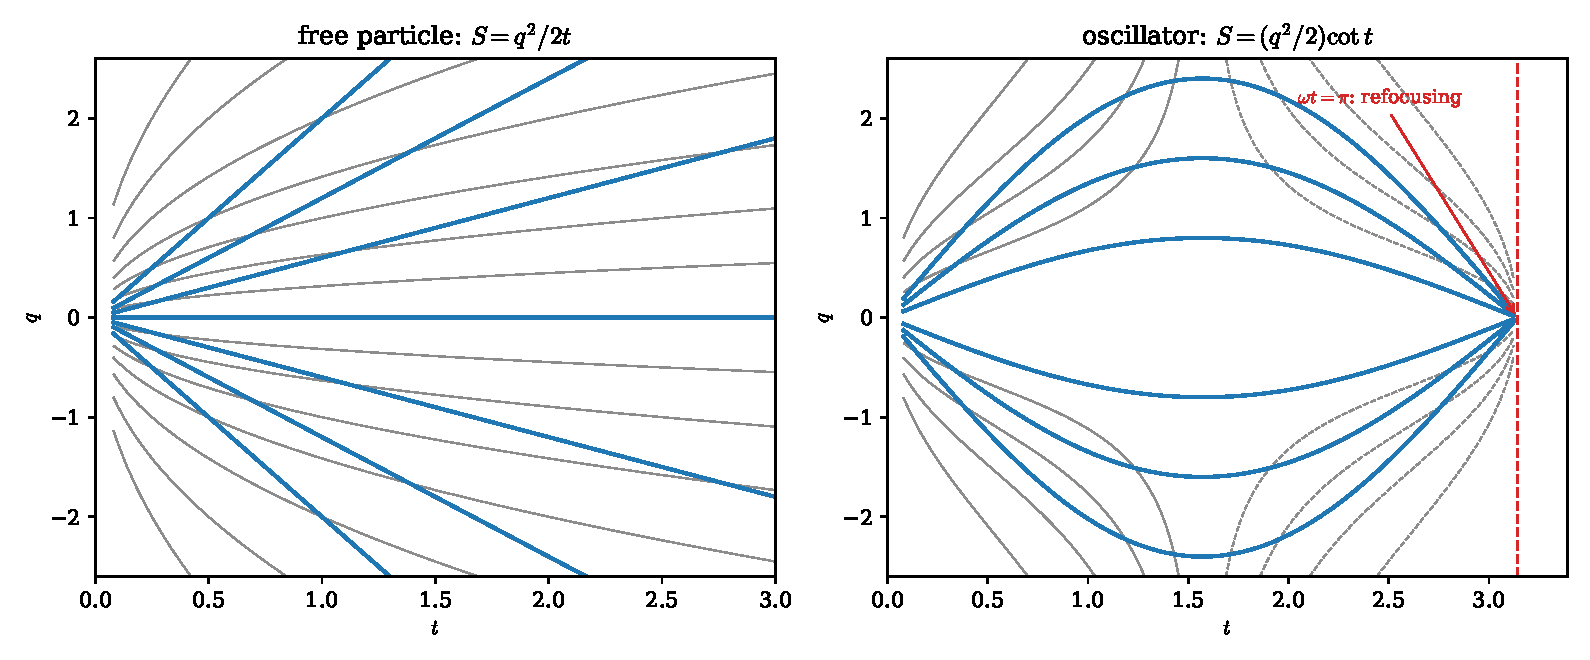
\includegraphics[width=0.95\textwidth]{fig_hj_action.pdf}
  \caption{Hamilton's principal function as a field over endpoints
  $(t, q)$, launched from $(q_0, t_0) = (0, 0)$; level sets of $S$
  (thin) with true trajectories (thick) crossing them. \emph{Left:}
  free particle, $S = m q^2/2t$ (Eq.~\eqref{eq:free-principal} with
  $q_0 = 0$), trajectories $q = vt$; every endpoint with $t > 0$ is
  reached by exactly one trajectory. \emph{Right:} oscillator,
  $S = (m\omega q^2/2)\cot\omega t$
  (Eq.~\eqref{eq:sho-principal} with $q_0 = 0$), trajectories
  $q = A\sin\omega t$; all trajectories refocus at $\omega t = \pi$,
  where the endpoint map degenerates
  ($\partial^2 S/\partial q\,\partial q_0 = -m\omega/\sin\omega t \to
  \infty$) and the principal function ceases to exist --- the failure
  of the uniqueness hypothesis of \S\ref{sec:hj-action}, made visible.
  Parameters $m = \omega = 1$; both panels drawn from the exact
  formulas by the figure script, which also verifies both formulas
  against the Hamilton--Jacobi equation symbolically.}
  \label{fig:hj-action}
\end{figure}

The cross-derivative of \eqref{eq:sho-principal} is
\begin{equation}
  \frac{\partial^2 S}{\partial q\,\partial q_0}
  = -\,\frac{m\omega}{\sin\omega T} :
\end{equation}
nonzero whenever defined, but blowing up as $\omega T \to \pi$ --- and
at $\omega T = \pi$ the formula \eqref{eq:sho-bvp} fails outright.
The geometry behind the failure is in Fig.~\ref{fig:hj-action}: every
trajectory launched from $q_0 = 0$, regardless of amplitude, returns
to $q = 0$ at $\omega t = \pi$ (half a period --- isochrony again, the
same fact that made the small-angle clock honest in
\S\ref{sec:pendulum}). At that instant the endpoint $(0, \pi/\omega)$
is reached by \emph{every} trajectory and the endpoints
$(q \ne 0, \pi/\omega)$ by none: the unique-connection hypothesis
collapses, and with it the principal function. Such refocusing points
are called \emph{conjugate points} (in optics, \emph{caustics}), and
they are the honest boundary of this subsection's construction
[stated; the systematic theory belongs to the calculus of variations'
second-variation chapter].

\begin{remark}[The quantum pointer, made quantitative]
\label{rem:hj-quantum}
Write a complex field from the principal function,
$\psi(q, t) = \ee^{\ii S(q,t)/\hbar}$, with $\hbar$ a constant
carrying the dimensions of action, and test it against the free
Schr\"odinger operator. Differentiate carefully:
\begin{equation}
  \ii\hbar\,\pd{\psi}{t} = -\pd{S}{t}\,\psi,
  \qquad
  -\frac{\hbar^2}{2m}\,\frac{\partial^2\psi}{\partial q^2}
  = \Bigl[\frac{1}{2m}\Bigl(\pd{S}{q}\Bigr)^{2}
    - \frac{\ii\hbar}{2m}\,\frac{\partial^2 S}{\partial q^2}
    \Bigr]\psi ,
\end{equation}
(the first term of the second bracket from the square of
$\partial_q S$, the second from the derivative acting twice ---
one power of $\hbar$ survives). Subtract, carrying a potential term $V\psi$ along on both sides:
\begin{equation}
  \ii\hbar\,\pd{\psi}{t}
  - \Bigl[-\frac{\hbar^2}{2m}\partial_q^2 + V\Bigr]\psi
  = -\underbrace{\Bigl[\pd{S}{t}
    + \frac{1}{2m}\Bigl(\pd{S}{q}\Bigr)^2 + V\Bigr]}_{=\;0
    \text{ by Hamilton--Jacobi}}\psi
  \;+\; \frac{\ii\hbar}{2m}\,\frac{\partial^2 S}{\partial q^2}\,\psi
  = \frac{\ii\hbar}{2m}\,\frac{\partial^2 S}{\partial q^2}\,\psi .
\end{equation}
The classical equation annihilates everything of order $\hbar^0$: the
Hamilton--Jacobi equation is what the Schr\"odinger equation becomes
when $\hbar$ is negligible against the actions in play, with the
residue --- one power of $\hbar$, proportional to $\partial_q^2 S$ ---
repaired by promoting the amplitude of $\psi$ to a second unknown
[stated; the systematic expansion is quantum mechanics' WKB
approximation]. This is the precise sense in which classical mechanics
is the stationary skeleton of a wave theory, and it dovetails with the
path-integral route of the quantum companion: there, each path is
weighted by exactly the phase $\ee^{\ii S/\hbar}$, and the classical
trajectory emerges by stationary phase [QM.\ \S10.3]. The function
this section extracted from the endpoint variation is the phase of the
quantum propagator.
\end{remark}

\begin{remark}[Beyond: action--angle variables, and the fence]
\label{rem:hj-beyond}
Two directions continue from here; both are pointed at, not entered.
\emph{First}, for bounded periodic motion the natural constant is not
$E$ but the phase-space area enclosed by the orbit --- the
\emph{action variable} $I = \oint p\,\dd q/2\pi$ whose first, unforced
appearance was the pendulum's $E/\omega_0$ in \S\ref{sec:pendulum-H},
and whose second was the conserved new momentum $P = E/\omega$ of the
oscillator example in \S\ref{sec:hj-gen}.
A complete integral built with $I$ as the new momentum makes the
conjugate \emph{angle} advance uniformly, and the pair $(I, \theta)$
is the natural language for slow perturbations (adiabatic invariants)
and for perturbation theory generally [stated; developed under the
name action--angle variables]. \emph{Second}, a fence: Jacobi's
theorem is local, and its global reach is a genuine dynamical
question. Complete integrals with global, single-valued $W$ exist
exactly when the system possesses $n$ independent conserved quantities
in involution --- the \emph{integrable} case [stated; the
Liouville--Arnold theorem] --- and the double pendulum at large
amplitude (\S\ref{sec:outlook}) is the standing reminder that this is
the exception, not the rule: no choice of coordinates untangles a
chaotic flow, and the Hamilton--Jacobi program, pushed against such a
system, fails not by technique but by theorem. What survives
universally is the local statement proved here, and the variational
identity $\dd S = \sum_i p_i\,\dd q_i - H\,\dd t$ that no amount of
chaos revokes.
\end{remark}

%=======================================================================
\section{Outlook}
%=======================================================================
\label{sec:outlook}

Three continuations are visible from here; this section only points
at them.

\paragraph{Beyond Hamilton--Jacobi.}
\S\ref{sec:hj} built canonical transformations and pushed them to the
$K = 0$ limit. The road continues: action--angle variables (the version
of the construction adapted to bounded periodic motion,
Remark~\ref{rem:hj-beyond}), adiabatic invariants, and canonical
perturbation theory --- the machinery for systems \emph{close} to
integrable, and the road on which the failures of integrability (KAM
theory, chaos) were first mapped [all stated at pointer level].

\paragraph{The double pendulum at large amplitude.}
Our \S\ref{sec:double-pendulum} lives in the quadratic basin. The exact
system \eqref{eq:dp-exact-1}--\eqref{eq:dp-exact-2} at higher energy is
the standard laboratory example of \emph{chaos}: deterministic,
energy-conserving (Liouville and $H$-conservation hold exactly), yet with
neighboring initial conditions separating exponentially fast, so that
long-term prediction fails in practice while the phase-space structure
theorems continue to hold. That these two facts coexist --- perfect
determinism, practical unpredictability --- is a central lesson of
twentieth-century mechanics, and the double pendulum is its cheapest
demonstration: two rods, two bobs.

\paragraph{Not covered.}
Rigid-body motion and velocity-dependent potentials (the charged
particle's $L = \tfrac12 m\dot{\vr}^2 - q\phi + q\,\dot{\vr}\cdot
\vec A$, the classical seed of gauge coupling) fit the framework
built here without modification; non-holonomic constraints (rolling)
genuinely require more [all three stated at pointer level].

\paragraph{The bracket becomes a commutator.}
The remark closing \S\ref{sec:poisson} leads directly into quantum
mechanics:
the Hamiltonian formalism is the classical half of a correspondence in
which Poisson brackets become commutators and the phase-space flow becomes
unitary evolution. Nothing in Parts I--II has to be unlearned; it has to
be \emph{deformed}, with $\hbar$ as the deformation parameter.

\appendix

%=======================================================================
\section{Differentiation Under the Integral Sign}
%=======================================================================
\label{app:diff-under-integral}

\begin{theorem}[Leibniz rule, the case used in \S\ref{sec:EL}]
Let $f(x,\varepsilon)$ and $\partial f/\partial\varepsilon$ be continuous
on $[a,b]\times[-\delta,\delta]$. Then
$\Phi(\varepsilon) = \int_a^b f(x,\varepsilon)\,\dd x$ is differentiable
and
\begin{equation}
  \Phi'(\varepsilon) = \int_a^b \pd{f}{\varepsilon}(x,\varepsilon)\,\dd x .
\end{equation}
\end{theorem}

\begin{proof}
Fix $\varepsilon$; for $h \neq 0$ small,
\begin{equation}
  \frac{\Phi(\varepsilon+h)-\Phi(\varepsilon)}{h}
  - \int_a^b \pd f\varepsilon(x,\varepsilon)\,\dd x
  = \int_a^b \left[\frac{f(x,\varepsilon+h) - f(x,\varepsilon)}{h}
  - \pd f\varepsilon(x,\varepsilon)\right]\dd x .
\end{equation}
By the mean value theorem in $\varepsilon$, for each $x$ there is
$\xi_x$ between $\varepsilon$ and $\varepsilon+h$ with
\begin{equation}
  \frac{f(x,\varepsilon+h)-f(x,\varepsilon)}{h}
  = \pd f\varepsilon(x, \xi_x),
\end{equation}
so the bracket equals
$\partial_\varepsilon f(x,\xi_x) - \partial_\varepsilon f(x,\varepsilon)$
with $|\xi_x - \varepsilon| \le |h|$. Now the one analytic fact:
$\partial_\varepsilon f$ is continuous on the \emph{compact} set
$[a,b]\times[-\delta,\delta]$, hence \emph{uniformly} continuous there.
Given $\epsilon' > 0$ choose $h$ small enough that
$|\partial_\varepsilon f(x,\xi) - \partial_\varepsilon f(x,\varepsilon)|
< \epsilon'$ whenever $|\xi - \varepsilon| \le |h|$, \emph{uniformly in
$x$}. The integral is then bounded by $(b-a)\,\epsilon'$, which proves the
limit.
\end{proof}

In \S\ref{sec:EL} this is applied with
$f(x,\varepsilon) = F(x,\, y+\varepsilon\eta,\, y'+\varepsilon\eta')$:
$F \in C^2$ and $y, \eta \in C^2$ make $f$ and $\partial_\varepsilon f$
continuous on the required compact rectangle.

%=======================================================================
\section{The Fundamental Lemma: Full Proof}
%=======================================================================
\label{app:fundamental-lemma}

\begin{lemma}
Let $g$ be continuous on $[a,b]$ and suppose
$\int_a^b g\,\eta\,\dd x = 0$ for every $\eta \in C^2([a,b])$ with
$\eta(a)=\eta(b)=0$. Then $g \equiv 0$ on $[a,b]$.
\end{lemma}

\begin{proof}
Suppose not: $g(x_0) \neq 0$ for some $x_0$; without loss of generality
$g(x_0) = 2c > 0$ (else replace $g$ by $-g$, permissible since $-\eta$ is
also a test function). By continuity there is a closed interval
$[\alpha,\beta] \subset (a,b)$ containing $x_0$ on which $g \ge c > 0$.
Construct the explicit bump
\begin{equation}
  \eta(x) =
  \begin{cases}
    (x - \alpha)^3\,(\beta - x)^3, & x \in [\alpha, \beta],\\[2pt]
    0, & \text{otherwise}.
  \end{cases}
\end{equation}
\emph{Admissibility}: $\eta$ vanishes at $a$ and $b$ (its support is
inside $(a,b)$); it is $C^2$ across the seams $x = \alpha, \beta$ because
each factor has a \emph{triple} zero there, so $\eta$, $\eta'$, $\eta''$
all vanish from inside, matching the zero function outside (a cubic-order
zero leaves two derivatives intact). \emph{Positivity}: $\eta > 0$ on the
open interval $(\alpha,\beta)$. Then
\begin{equation}
  \int_a^b g\,\eta\;\dd x
  = \int_\alpha^\beta g\,\eta\;\dd x
  \;\ge\; c\int_\alpha^\beta \eta\;\dd x \;>\; 0 ,
\end{equation}
contradicting the hypothesis. Hence $g \equiv 0$.
\end{proof}

(If test functions are required merely continuous or $C^1$, the same bump
works \emph{a fortiori}; if $C^\infty$ test functions are demanded,
replace the cubic factors by the standard
$\exp\bigl(-1/(x-\alpha)\bigr)\exp\bigl(-1/(\beta - x)\bigr)$ bump.)

%=======================================================================
\section{Covariance of the Euler--Lagrange Equations: Proof}
%=======================================================================
\label{app:covariance}

\emph{Setting} (Theorem~\ref{thm:covariance}): $q_i = q_i(\vec Q, t)$, a
$C^2$ change of coordinates with invertible Jacobian
$J_{ij} = \partial q_i/\partial Q_j$, and
$\widetilde L(\vec Q, \dot{\vec Q}, t)
= L\bigl(q(\vec Q,t),\, \dot q(\vec Q, \dot{\vec Q}, t),\, t\bigr)$, where
velocities transform by the chain rule
\begin{equation}
  \dot q_i = \sum_j \pd{q_i}{Q_j}\,\dot Q_j + \pd{q_i}{t} .
  \label{eq:velocity-transform}
\end{equation}

\begin{proof}
Two identities, precisely the (K1)--(K2) of \S\ref{sec:constraints} with
$\vr \to q$ and $q \to Q$, both read off \eqref{eq:velocity-transform}:
\begin{equation}
  \text{(K1)}\;\; \pd{\dot q_i}{\dot Q_j} = \pd{q_i}{Q_j},
  \qquad
  \text{(K2)}\;\; \frac{\dd}{\dd t}\pd{q_i}{Q_j} = \pd{\dot q_i}{Q_j}
\end{equation}
--- (K1) because $\dot Q_j$ enters linearly; (K2) because both sides equal
$\sum_k \frac{\partial^2 q_i}{\partial Q_k \partial Q_j}\dot Q_k
+ \frac{\partial^2 q_i}{\partial t\,\partial Q_j}$ (mixed partials of the
$C^2$ map commute). Now compute the $Q_j$ Euler--Lagrange expression of
$\widetilde L$ by the chain rule. Momentum slot:
\begin{equation}
  \pd{\widetilde L}{\dot Q_j}
  = \sum_i \pd{L}{\dot q_i}\,\pd{\dot q_i}{\dot Q_j}
  \overset{\text{(K1)}}{=}
  \sum_i \pd{L}{\dot q_i}\,\pd{q_i}{Q_j} ,
\end{equation}
\begin{equation}
  \frac{\dd}{\dd t}\pd{\widetilde L}{\dot Q_j}
  = \sum_i \left[\frac{\dd}{\dd t}\pd{L}{\dot q_i}\right]\pd{q_i}{Q_j}
  + \sum_i \pd{L}{\dot q_i}\,\frac{\dd}{\dd t}\pd{q_i}{Q_j}
  \overset{\text{(K2)}}{=}
  \sum_i \left[\frac{\dd}{\dd t}\pd{L}{\dot q_i}\right]\pd{q_i}{Q_j}
  + \sum_i \pd{L}{\dot q_i}\,\pd{\dot q_i}{Q_j} .
\end{equation}
Coordinate slot:
\begin{equation}
  \pd{\widetilde L}{Q_j}
  = \sum_i \pd{L}{q_i}\,\pd{q_i}{Q_j}
  + \sum_i \pd{L}{\dot q_i}\,\pd{\dot q_i}{Q_j} .
\end{equation}
Subtract: the $\partial L/\partial\dot q_i \cdot
\partial\dot q_i/\partial Q_j$ sums cancel, leaving
\begin{equation}
  \frac{\dd}{\dd t}\pd{\widetilde L}{\dot Q_j} - \pd{\widetilde L}{Q_j}
  = \sum_i \left[\frac{\dd}{\dd t}\pd{L}{\dot q_i} - \pd{L}{q_i}\right]
  \pd{q_i}{Q_j} .
  \label{eq:covariance-identity}
\end{equation}
The new Euler--Lagrange expressions are the old ones contracted with the
Jacobian. Since the Jacobian is invertible, the left side vanishes for all
$j$ \emph{iff} the bracket vanishes for all $i$.
\end{proof}

Equation \eqref{eq:covariance-identity} says more than the theorem: the
Euler--Lagrange expression transforms as a \emph{covector} under point
transformations --- the differential-geometric identity behind the slogan
``the equations are tensorial.''

%=======================================================================
\section{The Isoperimetric Multiplier Rule: Proof}
%=======================================================================
\label{app:isoperimetric}

\emph{Setting} (Theorem~\ref{thm:isoperimetric}): $y_\ast$ stationary for
$J$ subject to $\Lambda[y] = L$; $y_\ast$ not an unconstrained extremal of
$\Lambda$. Write, for test functions $\eta$,
\begin{equation}
  A[\eta] \equiv \delta J[y_\ast;\eta],
  \qquad
  B[\eta] \equiv \delta\Lambda[y_\ast;\eta]
\end{equation}
(both are integrals of the Euler--Lagrange--type bracket against $\eta$,
by Moves 1--3 of Theorem~\ref{thm:EL}'s proof).

\begin{proof}
Since $y_\ast$ is not an extremal of $\Lambda$, the fundamental lemma read
backwards supplies a test function $\eta_2$ with
$B[\eta_2] \neq 0$; normalize $B[\eta_2] = 1$. Fix an arbitrary test
function $\eta_1$ and consider the two-parameter family
\begin{equation}
  y_{\varepsilon_1,\varepsilon_2}
  = y_\ast + \varepsilon_1\eta_1 + \varepsilon_2\eta_2,
  \qquad
  \psi(\varepsilon_1,\varepsilon_2)
  \equiv \Lambda[y_{\varepsilon_1,\varepsilon_2}] - L .
\end{equation}
Then $\psi(0,0) = 0$ and
$\partial\psi/\partial\varepsilon_2(0,0) = B[\eta_2] = 1 \neq 0$, so the
implicit function theorem yields a $C^1$ function
$\varepsilon_2 = e(\varepsilon_1)$ near $0$ with $e(0) = 0$,
$\psi(\varepsilon_1, e(\varepsilon_1)) \equiv 0$, and
\begin{equation}
  e'(0)
  = -\,\frac{\partial\psi/\partial\varepsilon_1}
           {\partial\psi/\partial\varepsilon_2}\bigg|_{(0,0)}
  = -\,B[\eta_1] .
\end{equation}
The curve $\varepsilon_1 \mapsto y_{\varepsilon_1, e(\varepsilon_1)}$ is a
one-parameter family of \emph{admissible} (constraint-respecting)
competitors through $y_\ast$; stationarity of $J$ among admissible curves
gives
\begin{equation}
  0 = \left.\frac{\dd}{\dd\varepsilon_1}\right|_0
  J\bigl[y_{\varepsilon_1, e(\varepsilon_1)}\bigr]
  = A[\eta_1] + A[\eta_2]\;e'(0)
  = A[\eta_1] - A[\eta_2]\,B[\eta_1] .
\end{equation}
Set $\lambda \equiv -A[\eta_2]$ --- a single constant, fixed once by
$\eta_2$ and independent of $\eta_1$. The display reads
\begin{equation}
  A[\eta_1] + \lambda\,B[\eta_1] = 0
  \qquad\text{for \emph{every} test function } \eta_1 ,
\end{equation}
i.e.\ $\delta\bigl(J + \lambda\Lambda\bigr)[y_\ast;\eta_1] = 0$ for all
$\eta_1$: $y_\ast$ is an unconstrained stationary point of
$\int (F + \lambda G)\,\dd x$, and the Euler--Lagrange equation of
$F + \lambda G$ follows by Theorem~\ref{thm:EL}.
\end{proof}

%=======================================================================
\section{Simultaneous Diagonalization: Proof}
%=======================================================================
\label{app:simultaneous}

\emph{Setting} (Theorem~\ref{thm:simultaneous}): $\mM$ symmetric positive
definite, $\mK$ symmetric, both real $n\times n$; the problem
$\mK\vec v = \omega^2 \mM \vec v$.

\begin{proof}
\emph{Step 1: the square root.} By the spectral theorem [stated; the
spectral theorem of linear algebra], $\mM = O^{\mathsf
T} D\, O$ with $O$ orthogonal and $D = \mathrm{diag}(d_1,\dots,d_n)$,
$d_i > 0$ (positive definiteness). Define
$\mM^{1/2} \equiv O^{\mathsf T} D^{1/2} O$: symmetric, positive definite,
invertible, and $(\mM^{1/2})^2 = \mM$.

\emph{Step 2: reduce to an ordinary symmetric problem.} Substitute
$\vec w = \mM^{1/2}\vec v$ in the generalized problem:
\begin{equation}
  \mK\,\mM^{-1/2}\vec w = \omega^2\,\mM^{1/2}\vec w
  \quad\Longleftrightarrow\quad
  \underbrace{\mM^{-1/2}\,\mK\,\mM^{-1/2}}_{\equiv\,\mathsf A}\;\vec w
  = \omega^2\,\vec w ,
\end{equation}
and $\mathsf A$ is symmetric
($\mathsf A^{\mathsf T} = \mM^{-1/2}\mK^{\mathsf T}\mM^{-1/2} = \mathsf A$
since $\mM^{-1/2}$, $\mK$ are). The spectral theorem, invoked once
more, gives an
orthonormal basis $\vec w_1,\dots,\vec w_n$ of eigenvectors with real
eigenvalues $\omega_r^2$.

\emph{Step 3: translate back.} Set $\vec v_r = \mM^{-1/2}\vec w_r$: a
basis (image of a basis under an invertible map), solving the generalized
problem, with the claimed orthogonality
\begin{equation}
  \vec v_r^{\mathsf T}\,\mM\,\vec v_s
  = \vec w_r^{\mathsf T}\mM^{-1/2}\,\mM\,\mM^{-1/2}\vec w_s
  = \vec w_r^{\mathsf T}\vec w_s = \delta_{rs} .
\end{equation}
If $\mK$ is positive definite, the eigenvalues are positive:
$\omega_r^2 = \vec w_r^{\mathsf T}\mathsf A\,\vec w_r
= (\mM^{-1/2}\vec w_r)^{\mathsf T}\mK\,(\mM^{-1/2}\vec w_r)
= \vec v_r^{\mathsf T}\mK\,\vec v_r > 0$.

\emph{Step 4: decoupling.} Expand $\vth(t) = \sum_r \xi_r(t)\,\vec v_r$
and insert into $\mM\ddot\vth = -\mK\vth$; multiply on the left by
$\vec v_s^{\mathsf T}$. Using $\mK\vec v_r = \omega_r^2\mM\vec v_r$ and
then $\mM$-orthonormality,
\begin{equation}
  \sum_r \ddot\xi_r\,\vec v_s^{\mathsf T}\mM\vec v_r
  = -\sum_r \xi_r\,\omega_r^2\,\vec v_s^{\mathsf T}\mM\vec v_r
  \quad\Longrightarrow\quad
  \ddot\xi_s = -\,\omega_s^2\,\xi_s
  \qquad (s = 1,\dots,n) . \qedhere
\end{equation}
\end{proof}

%=======================================================================
\section{The Jacobi Identity: Computation}
%=======================================================================
\label{app:jacobi}

We verify
$\mathcal J \equiv \{f,\{g,h\}\} + \{g,\{h,f\}\} + \{h,\{f,g\}\} = 0$ for
one degree of freedom; the $n$-degree case is the identical computation
repeated for each index pair, since the bracket is a sum over $i$ of
identical one-pair blocks. Write partials as subscripts
($f_q = \partial f/\partial q$, $f_{qp} = \partial^2 f/\partial
q\,\partial p$, etc.), and recall $f_{qp} = f_{pq}$ throughout ($C^2$).

\paragraph{The organizing observation.}
Each double bracket expands into terms containing exactly \emph{one}
second derivative (of the innermost functions) times two first
derivatives. Sort all terms of $\mathcal J$ into three groups by which
function carries the second derivative; we show each group cancels on its
own. By the cyclic symmetry of $\mathcal J$, it suffices to check the
group of second derivatives of $f$ --- the other two follow by relabeling.

\paragraph{The expansion.}
From $\{g,h\} = g_q h_p - g_p h_q$:
\begin{align}
  \{f,\{g,h\}\}
  &= f_q\,\partial_p\bigl(g_qh_p - g_ph_q\bigr)
   - f_p\,\partial_q\bigl(g_qh_p - g_ph_q\bigr) \nonumber\\
  &= f_q\bigl(g_{qp}h_p + g_qh_{pp} - g_{pp}h_q - g_ph_{qp}\bigr)
   - f_p\bigl(g_{qq}h_p + g_qh_{pq} - g_{pq}h_q - g_ph_{qq}\bigr) .
\end{align}
No second derivative of $f$ appears here --- $f$ sits outside. Second
derivatives of $f$ arise only from the two brackets in which $f$ is
inside:
\begin{align}
  \{g,\{h,f\}\}\Big|_{f''\text{-terms}}
  &= g_q\bigl(h_q f_{pp} - h_p f_{qp}\bigr)
   - g_p\bigl(h_q f_{pq} - h_p f_{qq}\bigr) ,\\
  \{h,\{f,g\}\}\Big|_{f''\text{-terms}}
  &= h_q\bigl(f_{qp}\,g_p - f_{pp}\,g_q\bigr)
   - h_p\bigl(f_{qq}\,g_p - f_{pq}\,g_q\bigr) .
\end{align}
Add and collect by second-derivative type:
\begin{align}
  f_{pp}:&\quad g_q h_q - h_q g_q = 0, \nonumber\\
  f_{qq}:&\quad g_p h_p - h_p g_p = 0, \nonumber\\
  f_{qp} = f_{pq}:&\quad
  \bigl(-g_q h_p\bigr) + \bigl(-g_p h_q\bigr)
  + \bigl(h_q g_p\bigr) + \bigl(h_p g_q\bigr) = 0 .
\end{align}
Every coefficient vanishes --- crucially using $f_{qp} = f_{pq}$ to merge
the mixed terms; the Jacobi identity is, at bottom, \emph{the symmetry of
second derivatives}, three times over. The $g''$- and $h''$-groups vanish
by the cyclic relabelings $(f,g,h) \to (g,h,f) \to (h,f,g)$, and with all
second-derivative groups zero and no other terms present,
$\mathcal J = 0$.

\end{document}
